\documentclass{article}
\usepackage{listings}
\usepackage{minted}
\usepackage{lipsum}
\usepackage[a4paper, margin=1.4in]{geometry}
\usepackage{float}
\usepackage{amsmath}
\usepackage{hanging}
\usepackage{xcolor}
\usepackage{textcomp}
\usepackage{tikz}
\usetikzlibrary{calc}
\usepackage{graphicx}
\usepackage{setspace}
\usepackage{subcaption}
\usepackage[utf8]{inputenc}

\graphicspath{ {./thesisimages/} }

\usepackage{fontspec}
\setmainfont{Minion Pro}


\begin{document}
\setlength{\parindent}{0in}
\setlength{\parskip}{\baselineskip}

\begin{titlepage}

\begin{tikzpicture}[overlay,remember picture]
    \draw [line width=1pt,rounded corners=0pt,
        ]
        ($ (current page.north west) + (1.6cm,-1.6cm) $)
        rectangle
        ($ (current page.south east) + (-1.6cm,1.6cm) $);
\end{tikzpicture}

    \begin{center} 
	\Large
        \vspace*{1cm}
        
        \textbf{ Integrated Deep Learning and Bayesian Classification for Prioritization of Functional Genes in Next-Generation Sequencing Data }
        
        \vspace{0.5cm}
        %subtitle here
        
        \vspace{1.0cm}
        
        \textbf{Chan Khai Ern, Edwin}
        
\vspace{9.0cm}
        \normalsize
       A thesis submitted to the \\
Department of Biochemistry \\
National University of Singapore \\
in partial fulfilment for the \\
Degree of Bachelor of Science with \\Honours
in
Life Sciences\\

        
        \vspace{1.5cm}
        
        
        Life Sciences Honours Cohort \\
        AY2015/2016 S1\\
       
        
    \end{center}
\end{titlepage}
\newpage
\pagenumbering{Roman} 
\doublespace
\large
\vspace{50pt}
\begin{center}
\textbf{DECLARATION}\\[\baselineskip]
I hereby declare that this thesis is my original work and it has been written by me in its entirety. I have duly acknowledged all the sources of information which have been used in the thesis.\\[\baselineskip]
This thesis has also not been submitted for any degree in any university previously.\\[3\baselineskip]
\begin{center}
\line(1,0){150}
\end{center}
Chan Khai Ern Edwin\\
04 April 2017
\end{center}
\newpage
\section*{Acknowledgements}
\newpage
\section*{Table of Contents}
\large
\tableofcontents
\newpage
\doublespace
\large
\pagenumbering{arabic} 
\section*{Abstract}
The advent of next generation sequencing technology has enabled large scale interrogation of the genome to identify variants in patient samples. The accurate identification of functional variants can provide critical insights into the disease process to guide diagnosis and treatment. However, the use in clinical genomics remains limited as (i) the accurate identification of variants remains suboptimal, and (ii) the large number of variants identified may be difficult to interpret without a systematic approach of ranking by functional importance.\\\\
Here, we describe the development of a deep learning neural network to improve the accuracy of variant-calling, and a Bayesian classification method for the probabilistic ranking of functionally relevant genes. We show that an optimised neural network can call variants more accurately than single variant callers or concordant callers, with F1 score improvements of 6.5 percent in simulated datasets and 4.5 percent in real datasets over the best concordant methods. Following the identification of high confidence variants, we further demonstrate that a Bayesian classification system is able to rank functionally relevant genes in a Diffuse Large B-Cell Lymphoma (DLBCL) patient sample.\\\\
We propose that the combined use of deep learning and Bayesian network analysis could be extended to build analytical pipeline for clinical use to augment diagnosis and treatment of diseases by identifying high confidence variants and ranking them systematically.
\newpage
\section{Introduction}
\subsection{Next Generation Sequencing (NGS) for Clinical Genomics}
There has been a growing interest in using a patient's genome to guide the diagnosis and treatment of diseases (Rehm, 2017; Angrist, 2016), based on the fundamental intuition is that variants and mutations in the genome alter gene functions that drive the initiation and progression of the disease. In oncology, for example, identification of the key driver mutations has been shown to be useful in stratifying cancer subtypes (Stratton, Campbell \& Futreal, 2009), and identifying mutations for targeted therapy (Janitz, 2011). Furthermore,the development of next generation sequencing (NGS) technologies have dramatically reduced sequencing costs (Metzker, 2010; Mardis, 2008), enabling the adoption of genomic sequencing in clinical labs.

Although clinical genomics holds great promise, there are still two critical issues that limits its use in a clinical setting. Firstly, it is often difficult to obtain high-confidence variant calls from  sequencing data, and secondly, the large number of variant calls for patient samples makes  interpretation difficult for clinical decision-making.

\subsection{Variant Calling of NGS Data}
In variant calling, genomic DNA is fragmented and the short reads are sequenced in a massively parallel manner using next generation sequencing technologies such as sequencing by synthesis. These reads  are aligned to the reference genome and variations in the DNA sequence, such as single nucleotide variants (SNV) and insertions/deletions (indels) are identified by comparing the different reads aligned to the reference genome (Figure 1).

\begin{figure}[H]
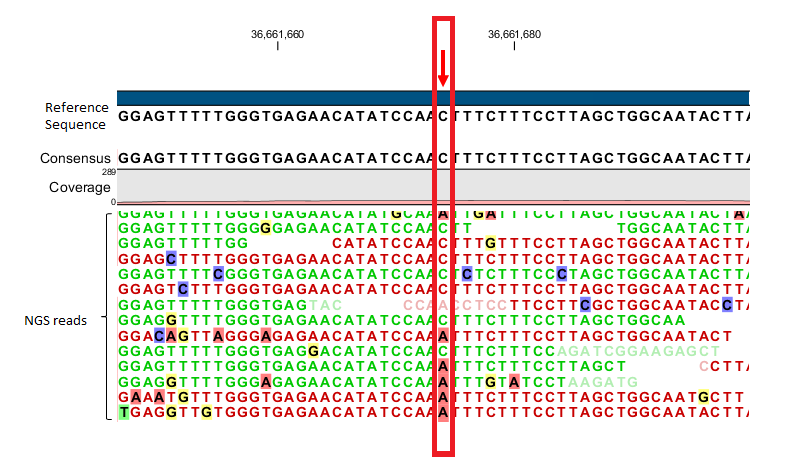
\includegraphics[width=\textwidth]{ngsreads.png}
\centering
\caption{Variant Calling Pileup - Due to noise and errors in sequencing and read mapping, it can be difficult to accurately call variants. Figure adapted from CLC Genomics Workbench 9.5, Figure 29.8.}
\end{figure}

Variant calling with NGS data primarily involves the use of various statistical and algorithmic methods to identify variants in the genome (Nielson et al., 2011). These variants represent the deviations and differences between the genome of interest and a reference human genome. This analysis is non-trivial as each variant call requires the integration of multiple sequence reads (e.g. millions of reads) that contain experimental noise and errors (Zook et al., 2014). The calling of variants can be further complicated by errors in mapping the reads to a reference genome.

 To account for these errors, variant callers employ a variety of algorithms and statistical models to determine the existence and type of variation/mutation (Zook et al., 2014; Davey et al., 2011). Because of the differences in assumptions and models employed by different variant callers, certain calling algorithms are more sensitive and accurate in calling specific classes of variants but do not perform well in calling other variant types (O'Rawe et al., 2013). To address these problems, ongoing efforts have focused on improving current variant calling algorithms, including optimization of variant calling for different classes of mutations, as well as reduction in the number of false positive calls (Mohiyuddin, et al., 2015; Gézsi et al., 2015). 

Despite the variety of approaches used for identifying variants and mutations,  the accuracy and precision of single variant callers  remains suboptimal (Cornish and Guda, 2015 ; O'Rawe et al., 2013). Each variant caller can differ greatly in accuracy depending on the type of sequencing methodology and statistical algorithm used (Figure 2), making it difficult to identify true high confidence variant calls.

\begin{figure}[H]
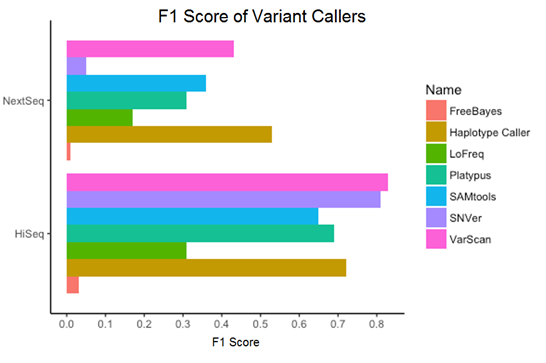
\includegraphics[width=\textwidth]{f1scorerealdatasets.png}
\centering
\caption{Performance of Variant Calling tools on Ratient Data using  Different Illumina Sequencing Platforms (HiSeq and NextSeq). The F1 score indicates how well a caller can predict true positives (See Appendix 5.3 for more details). Notably the F1 score for the same variant calling tool can differ greatly. Figure adapted from Sandmann et al. (2017)}
\end{figure}

\subsection{Ensemble Methods for Improving the Accuracy of Variant Calling} 

While it is clear that single variant callers may not perform well across a variety of variant classes, the combination or ensemble of several callers can be used to augment the accuracy of variant callers beyond what can be achieved with a single caller. By aggregating the calls from each different variant caller, the relatively weak prediction calls from each caller can be combined to provide a better aggregate prediction for a variant call. 

One simple approach to aggregating variant calls is concordance, where the likelihood of an accurate call depends on multiple variant callers identifying the same variant or mutation (Lam et al., 2012; Wei et al., 2011). While straightforward and intuitive, the recall rates of such a tool is poor with a high number of false negative calls. This is because a high concordance of variant calls will reciprocally decrease the number of true variants calls that are identified by specific variant callers (O'Rawe et al., 2013). 

Beyond concordance, supervised machine learning approaches have been used to combine the calls from different variant callers to improve the accuracy. In these approaches, machine learning algorithms have been used predict the accuracy of a variant call by integrating different features of each variant call (e.g. variant frequencies, mapping quality). For example, the support vector machine (SVM) algorithm was used successfully to improve the accuracy of variant calls (Gézsi et al., 2015) over concordance-based methods. 

Recent advances in machine learning, in particular deep learning neural networks, have increased the accuracy of predictions from complex multi-modal data (Ng et al., 2015) beyond traditional algorithms such as SVM and Random Forests. The ability of deep learning networks  to learn from complex high-dimensional data suggests that they may be useful in improving the accuracy of high confidence variant calls derived from the complex features from each variant caller. 

\subsection{Deep Learning for Improving the Accuracy of Variant Calling} 

Deep learning is a machine learning approach based on artificial neural networks (LeCun et al., 2015) built on artificial neurons. Each artificial neuron is analogous to a biological neuron where weighted input signals are integrated to produce an output once the signals cross a threshold for activation (Figure 3).  

\begin{figure}[H]
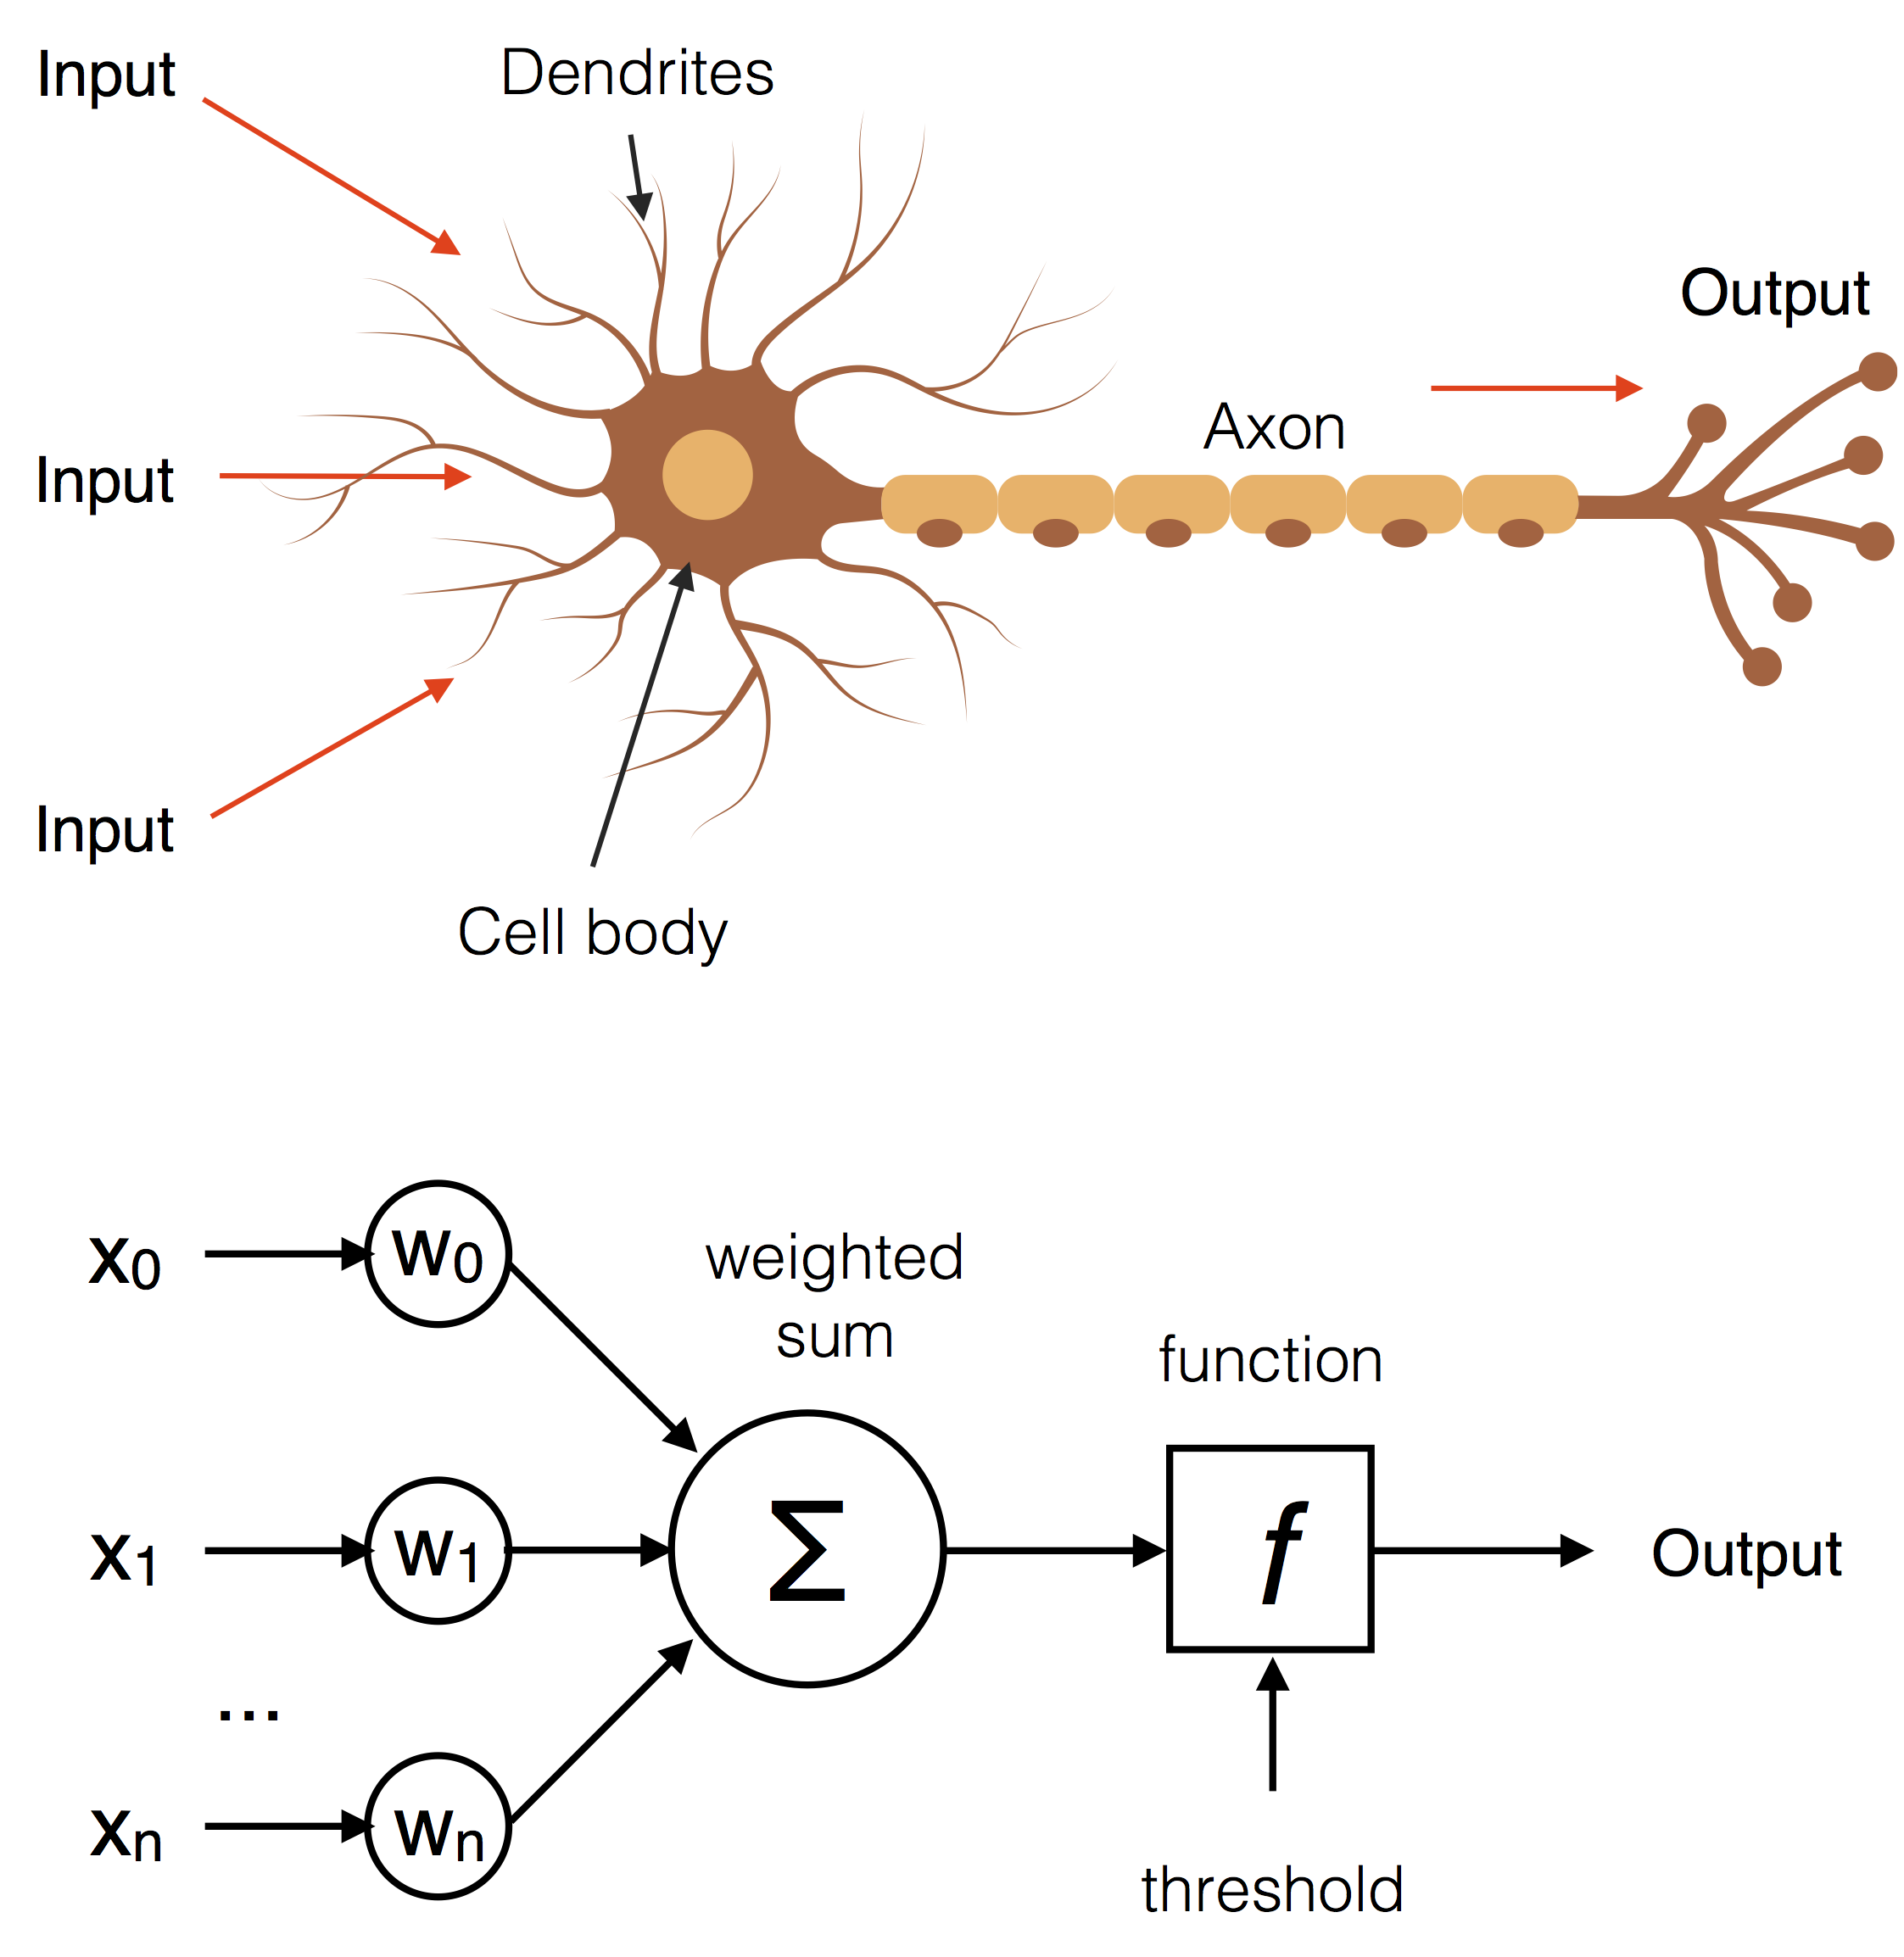
\includegraphics[width=0.8\textwidth]{neuron.png}
\centering
\caption{Artificial Neurons as Building Blocks of Neural Networks}
\end{figure}

[TO CONTINUE EDITING FROM HERE]

Deep learning networks are trained by providing the input data and output data and letting the network learn how to integrate the inputs to create a network of activations that can be used to produce the corresponding output. A more in-depth explanation into their algorithms can be found in Appendix 5.1. 

The output can be propagated to the next neuron depending on the weighted inputs.

By adjusting the weights that determine the propagation of a signal from one neuron to the next, the network can be adjusted to learn from labeled training data so that it can predict the output given new data.

Deep learning has been shown to be able to solve  complex non-linear decision boundary problems, including drug molecule solubility (Lusci et al., 2013), facial recognition (Sun et al., 2014) and even predicting the best move in the Japanese board game, Go (Silver et al., 2016). Figure 3 shows a typical neural network with 5 layers, including an input and output later.
\begin{figure}[H]
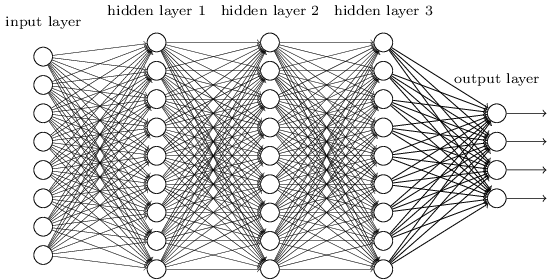
\includegraphics[width=\textwidth]{neuralnet.png}
\centering
\caption{A Neural Network with one input layer, three hidden layers and one output layer. This represents a densely connected neural network, where each node is connected to every node of the preceding and subsequent layers.}
\end{figure}


In variant calling, we hypothesise that deep learning will allow us to predict based on variant calling features and data whether a variant is valid and exists, or is erroneous. The deep learning network should be able to draw on the diversity of data with different variant callers and learn which patterns will result in a valid call and which patterns are false positives. It will also allow us to tap on the differential sensitivity of different callers, as the neural network is able to learn which callers work best for which types of mutations. Thus, we propose that deep learning as a combinatorial approach will allow us to improve the accuracy and precision of variant calling.
\subsection{Prioritisation of Variants with Bayesian Networks }
Once high confidence variant calls can be established, there remains the second problem of identifying the functional importance of each variant/mutation, given that there are multiple variants in a typical genome (Shen et al., 2013). The ability to systematically prioritize and rank clinically significant variants and mutations would allow clinicians to focus their attention on relevant candidate mutations that can guide decision-making on diagnosis and treatment.\\\\
The problem of prioritisation of genetic mutations arises from the multiplicity and complexity of data sources that can be utilized to determine the clinical and functional relevance of a variant ormutation in a gene (Moreau \& Tranchevent, 2012). Several approaches include studying previously characterised variants and their phenotypic effects on a person as well as how the mutation itself will affect protein function through studying the likelihood of amino acid mutation for conserved regions. These functional annotations can be done with the tool ANNOVAR (Wang, Li, \& Hakonarson, 2010) but the fundamental problem here is integrating such information in a systematic manner that is clear and understandable to clinicians. Clinicians may not be so familiar with the tools and functional annotation pipelines, and so for them to trust such a ranking system, they have to be able to understand intuitively how it works. \\\\
To solve this problem, we can use Bayesian networks to integrate the information from functional annotations as well as the confidence of a call (how likely it is real) to provide a ranking system for how likely the gene is going to be important. Bayesian networks were chosen for this ranking system as it is understandable and yet have proven stable in terms of solving decision-making problems (Pourret et al.,2008; Jensen et al., 1996). Bayesian networks have been applied in medical treatment decision making (Windecker et al., 2014), ecological studies (Johnson et al., 2014) and even predictive epidemiology (Su et al., 2014). A Bayesian network is a network that records the probabilities of events and based on conditional probabilities and observations it updates the final likelihood of an event. This can be seen in Figure 2.
\begin{figure}[H]
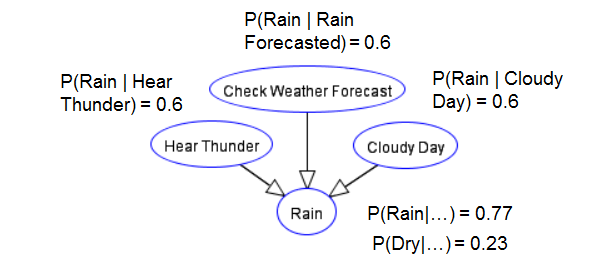
\includegraphics{samplebayesiannetwork.png}
\centering
\caption{A Sample Bayesian Network for Rain Prediction.}
\end{figure}
Here, we would like to predict how likely it is to rain. Thus, we record observations (we hear thunder, check the weather forecast, notice it is a cloudy day) and updating the likelihood of rain happening based on the conditional probabilities of P(Rain | Hear Thunder)... and so on. This model of learning was chosen because a Bayesian Network closely mimics the way humans think - we observe events and form co-relational and causative predictions based on those events. This is advantageous over deep learning as in deep learning we are unable to interrogate the system to understand intuitively what the network is learning form - it has high predictive power but is essentially a black-box. The Bayesian network allows clinicians and doctors to see what are the components that went into gene ranking and prioritisation, and even change the probabilities, weights or add more observation nodes based on their own diagnosis and treatment knowledge. Ultimately, this enables the doctors and clinicians to be able to have confidence in the software as they can analyse and understand how it works. This also allows them to be able to explain their methodology and treatment plans clearly to the patient, making the diagnosis and treatment process clear, understandable and transparent.

\subsection{Aims and Approach}

The overall goal of this thesis is to address the 2 major issues limiting the utility of clinical genomics through the following aims:

identification and prioritization of mutations in clinical samples

We describe the development of (i) a deep learning network to identify high-confidence variant calls (focusing on SNVs and short indels) and (i) a Bayesian network to probabilistically prioritise their functional importance. As a first step, we developed and optimized a deep learning network to identify true variants in both synthetic and real world datasets. Following the identification of high confidence variant calls,, we will build a Bayesian network based on functional annotations to prioritise mutations and test our network on a cancer dataset.

\newpage
\section{Materials and Methods}

\subsection{Overall Approach}
To enable the deep learning networks and Bayesian network analysis, we first built two main computational pipelines - the first pipeline is used to train and optimise a neural network, and the second pipeline uses a trained neural network to perform variant validation and prediction. Two pipelines are required as one pipeline is needed to train the network, and then the second pipeline can use the trained network to perform predictions. The first pipeline involves using a training dataset (either simulated or obtained from real sequencing data) and then performing processing steps of alignment, variant calling and finally deep learning network training and prediction on the dataset. This pipeline focuses on generate a set of predictions, and subsequently validating this set of predictions with a ground truth. The second analysis pipeline is meant for real datasets with in which the ground truth is not known, and so it uses a pre-trained neural network. For this pipeline, we perform similar steps of alignment and variant calling, and then use a trained neural network to predict which features are true. Finally, we can apply the Bayesian network analysis to predict the important genes in this dataset.

\begin{figure}[H]
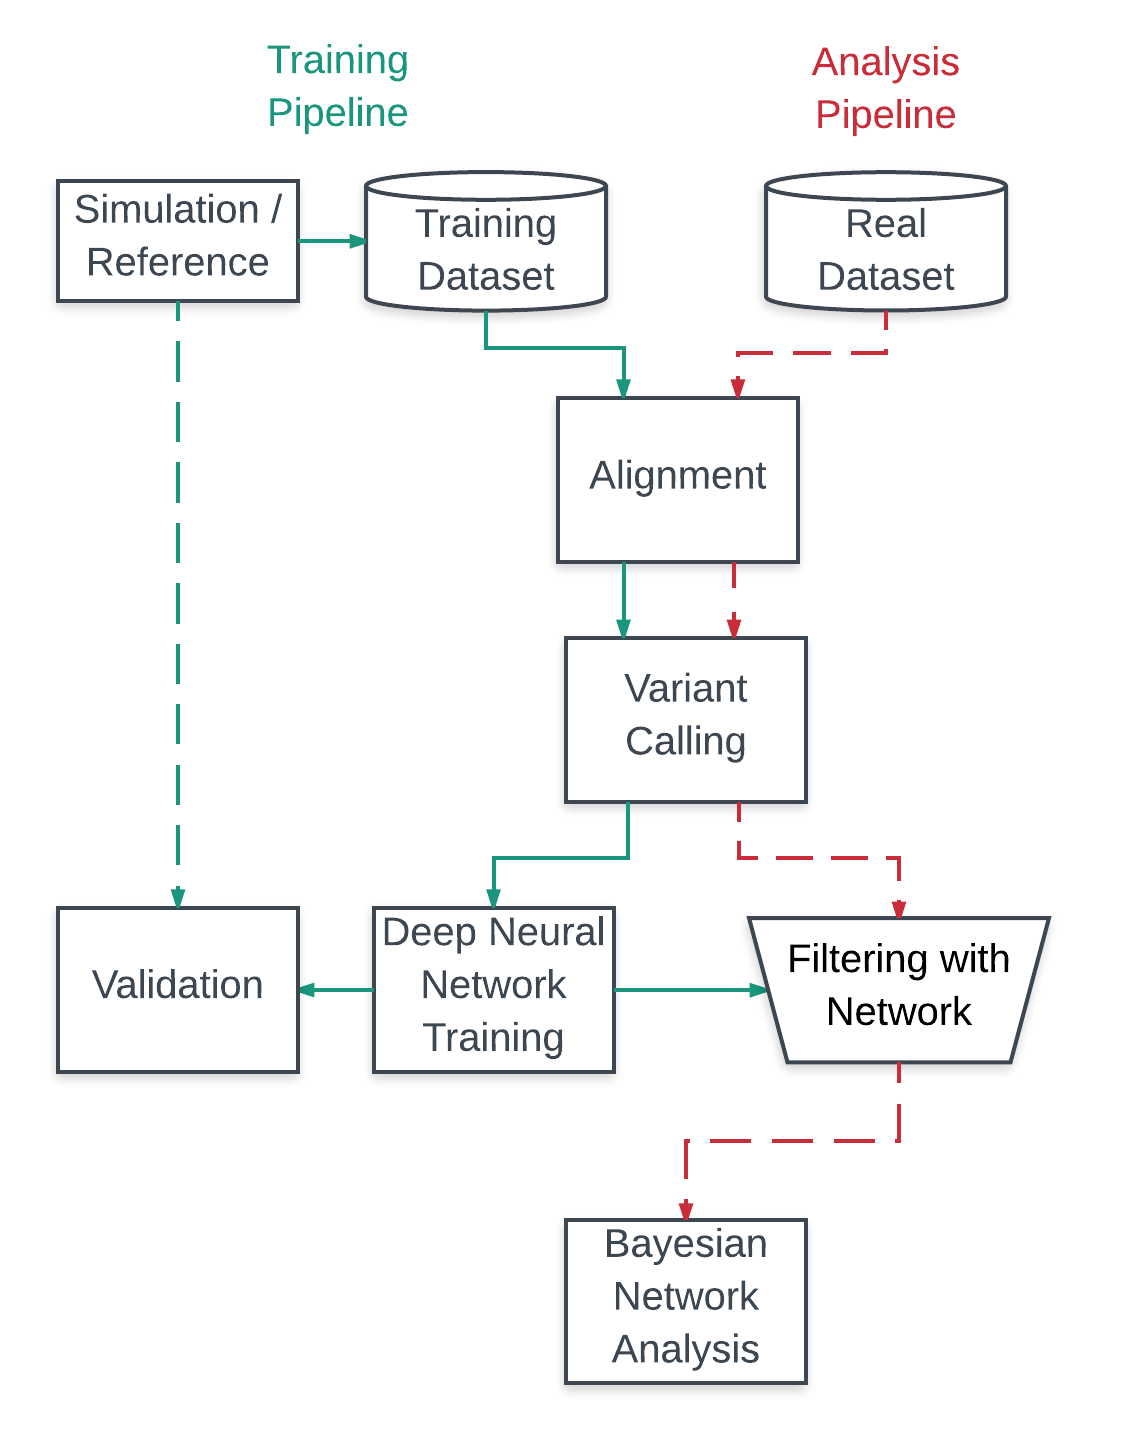
\includegraphics[width=\textwidth]{trainingpathway.png}
\centering
\caption{Overall Analytical Pipelines - Pipelines were implemented using the Groovy Domain Specific Language, NextFlow.}
\end{figure}

\subsection{Programming and Pipelining tools}

The general programming language used was Python (v2.7). Python was chosen due to its access to various important libraries, including NumPy, SciPy, Pomegranate and PyVCF. NumPy was used to prepare input vectors for deep learning training, SciPy was used to perform Principal Component Analysis and Synthetic Minority Oversampling Technique Methods (See Appendix 5.3 for more information). Finally, PyVCF was used to parse the VCF files into python objects for easy manipulation. Comparison of variants was also performed using python dictionary lookups. This method was chosen due to a high number of lookups required, and a fast O(1) constant time required for each lookup.\\\\
General pipelining and chaining of programmes was done using NextFlow and Bash scripts. NextFlow is a Groovy Based Domain Specific Language (DSL) that provides easy writing of parallel pipelines with an accessible unix interface. Nextflow was used to run the overall pipelines and control input and output of abstracted core modules, which are in turn either python scripts or Bash shell scripts. This ensures that results are easily replicable and can be later implemented as a single analytic pipeline for clinical use.\\\\
For our deep learning networks, we used the Keras library (v1.1.1) with a TensorFlow backend (v0.11.0). TensorFlow (Abadi et al., 2015) was chosen due to its distributed computation and queue management system that enabled better performance in training on a CentOS-7 compute cluster compared to other backends. For more explanation on the algorithms underpinning deep learning, see Appendix 5.1 for more information.\\\\
Finally, ANNOVAR was used to generate the functional annotations for the Bayesian probabilistic model. The protocols used were snp138, clinvar\_20150629 and ljb26\_all. Pomegranate (a Python library) was used to generate and compute the probabilistic model and ranking system for our Bayesian Network. For the probabilistic model, The preparation of the probabilistic model and the truth-tables required was done using Python scripts and subsequently used as input in pomegranate.

\subsection{Artificial Datasets}
Artificial genomes enable the simulation of NGS data with ground truths to test and validate a neural network. For our simulator, we used Mason, a genome mutation software written in C++ (SeqAn version 2.3.1) to mutate the hg19 reference genome from UCSC (Karolchik et al., 2014). We used indel rates of 0.00002 and SNP rates of 0.00008 to generate sufficient truth variants for analysis, which comprise 229253 SNPs and 57257 indels.\\\\
After generating a ground truth model, we simulated sequence reads with error rates and ground truth variants(Figure 5). For error rates, we used published data from Schirmer et al. (2016) as the input to Mason - the general substitution error rate used was 0.0004 per base in the genome, and the insertion and deletion error rate per base were $5*10^{-6}$.

\begin{figure}[H]
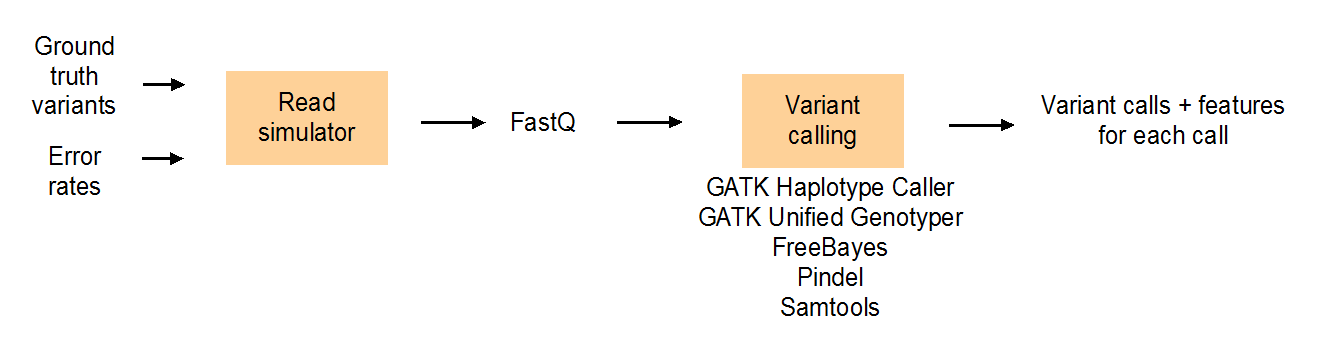
\includegraphics[width=\textwidth]{readsimulation.png}
\caption{Pipeline for simulation of artificial genome for analysis}
\centering
\end{figure}

\subsection{Alignment and Variant Calling} 
To perform alignment of simulated and real sequences, the Burrows-Wheeler Aligner (Li, 2013), version 0.7.13, was used. Default settings were used, with the mem option which is known to work well with longer sequences. After alignment, variant calling was performed. Variant callers used were FreeBayes (v1.0.2-16), GATK Haplotype Caller (v3.7-0) and Unified Genotyper (v3.7-0), Samtools (v1.3.1) and finally Pindel (v2.3.0)(Garrison \& Marth, 2012; McKenna et al. 2010, DePristo et al. 2011; Li H, et al., 2009; Ye et al., 2009). All callers were used at their default settings.

\subsection{Feature Engineering}
In order to train a neural network, features in the form of numerical vectors must be used an input. We subset our features into three broad sets, which are base-specific information, sequencing error and bias information features, and calling and mapping quality. Here we describe the computation of the features - please see Appendix 5.2 for a more in-depth explanation on their usage and interpretation.\\\\
\textbf{Base Information} \\[0.3\baselineskip]
\underline{Shannon Entropy}\\
Shannon Entropy captures the amount of information contained inside the allele sequences. It is calculated using the equation:
\begin{equation}
H(X) = -\sum_{i=1}^{n}P(x_i)\log_{2}P(x_i)
\end{equation}
where $P(x_i)$ is the prior probability of finding each base at each position. This prior probability is calculated in two ways - over the entire genome and over a region of space around the allele (10 bases plus the length of the allele in our calculations).\\[0.3\baselineskip]
\underline{Kullback Leibler Divergence}\\
The Kullback-Leibler Divergence feature is similar to Shannon entropy, but instead, we use this to measure the informational gain from the reference to the allele sequence. The Kullback-Leibler Divergence is calculated as follows:
\begin{equation}
D_{KL}(P||Q) = -\sum_{i=1}^{n}P(x_i)\log_{2}{\frac{P(x_i)}{Q(x_i)}}
\end{equation}
where $Q(x_i)$ is the prior probability of finding each base at each position based on the genomic region around the allele, while $P(X_i)$ is the posterior probability of finding a specific base inside the allelic sequence.\\[0.3\baselineskip]
\underline{Base Quality}\\
Base quality refers to the Phred score probability that the called allele is wrong. It is given by the equation:
\[ \scalebox{1.2}{$P=10^{\frac{-Q}{10}}$} \]
Where P is the Base Quality, and Q is the probability that the allele called is wrong. This is a number computed by the sequencing machine based on the quality of the base samples provided.\\\\
\textbf{Sequencing Biases and Errors} \\[0.3\baselineskip]
\underline{GC content}\\
This feature comprises the percentage GC content of reference genome for at least ten bases around the mutation site.\\[0.3\baselineskip]
\underline{Longest homozygous run}\\
This feature comprises the longest similar string of bases in the reference genome, for at least ten bases around the mutation site.\\[0.3\baselineskip]
\underline{Allele Count and Allele Balance}\\
This feature is an output from Haplotype Caller and Unified Genotyper, and describes the total number of alleles contributing to a call and the balance between reference and alternate alleles reads.\\\\
\textbf{Calling and Mapping Qualities} \\[0.3\baselineskip]
\underline{Genotype Likelihood}\\
The genotype likelihood score provides the Phred-scaled likelihood scores of how confident the caller is in determining that it is a homozygous or heterozygous call, and is provided by all variant callers.\\[0.3\baselineskip]
\underline{Read Depth}\\
Mapped read depth refers to the total number of bases sequenced and aligned at a given reference base position. It is provided by all variant callers.\\[0.3\baselineskip]
\underline{Quality by Depth}\\*
Quality by Depth is computed by dividing the quality score against allele depth, to obtain an average score of allele quality. This is provided by Haplotype Caller and Unified Genotyper.\\[0.3\baselineskip]
\underline{Mapping Quality}\\
Mapping quality is a score provided by the alignment method and gives the probability that a read is placed accurately. It is provided by all variant callers except Pindel.\\


\subsection{Patient Derived Xenograft Mouse Model Development and Sequencing}
[TO CLARIFY] To test the Bayesian ranking system, we used a patient-derived xenograft mouse model. Athymic mice with the FOX mutation were grown for X number of days, and subsequently, a tumour is grafted onto the mouse's body. Subsequently, the tumour was sequenced on an Illumina MiSeq platform and used for analysis. 

\newpage
\section{Results}
\subsection{Generation of Artificial Datasets}
Using a genome mutation software, we generated a mutated genome using the hg19 genome from UCSC (Karolchik et al., 2014) as a reference. The mutated genome contains over 300,000 random mutations spread over the chromosomes as can be seen below in Figures 3 and 4. Artificial genomes are a good method to analyse deep learning networks on as the ground truth, which are the truth variants inside the genome, are already known. This allows accurate verification of prediction schemes and is a commonly used method to test next generation sequencing related software (Escalona, Rocha \& Posada, 2016). This is primarily because it is difficult to obtain complete truth datasets for real genomes as due to the inhibitory cost of checking every variant called via Sanger sequencing. Thus, artificial genomes present a simple way to simulate NGS data with perfectly known ground truth variants to test our validation platform.

\begin{figure}[H]
\centering
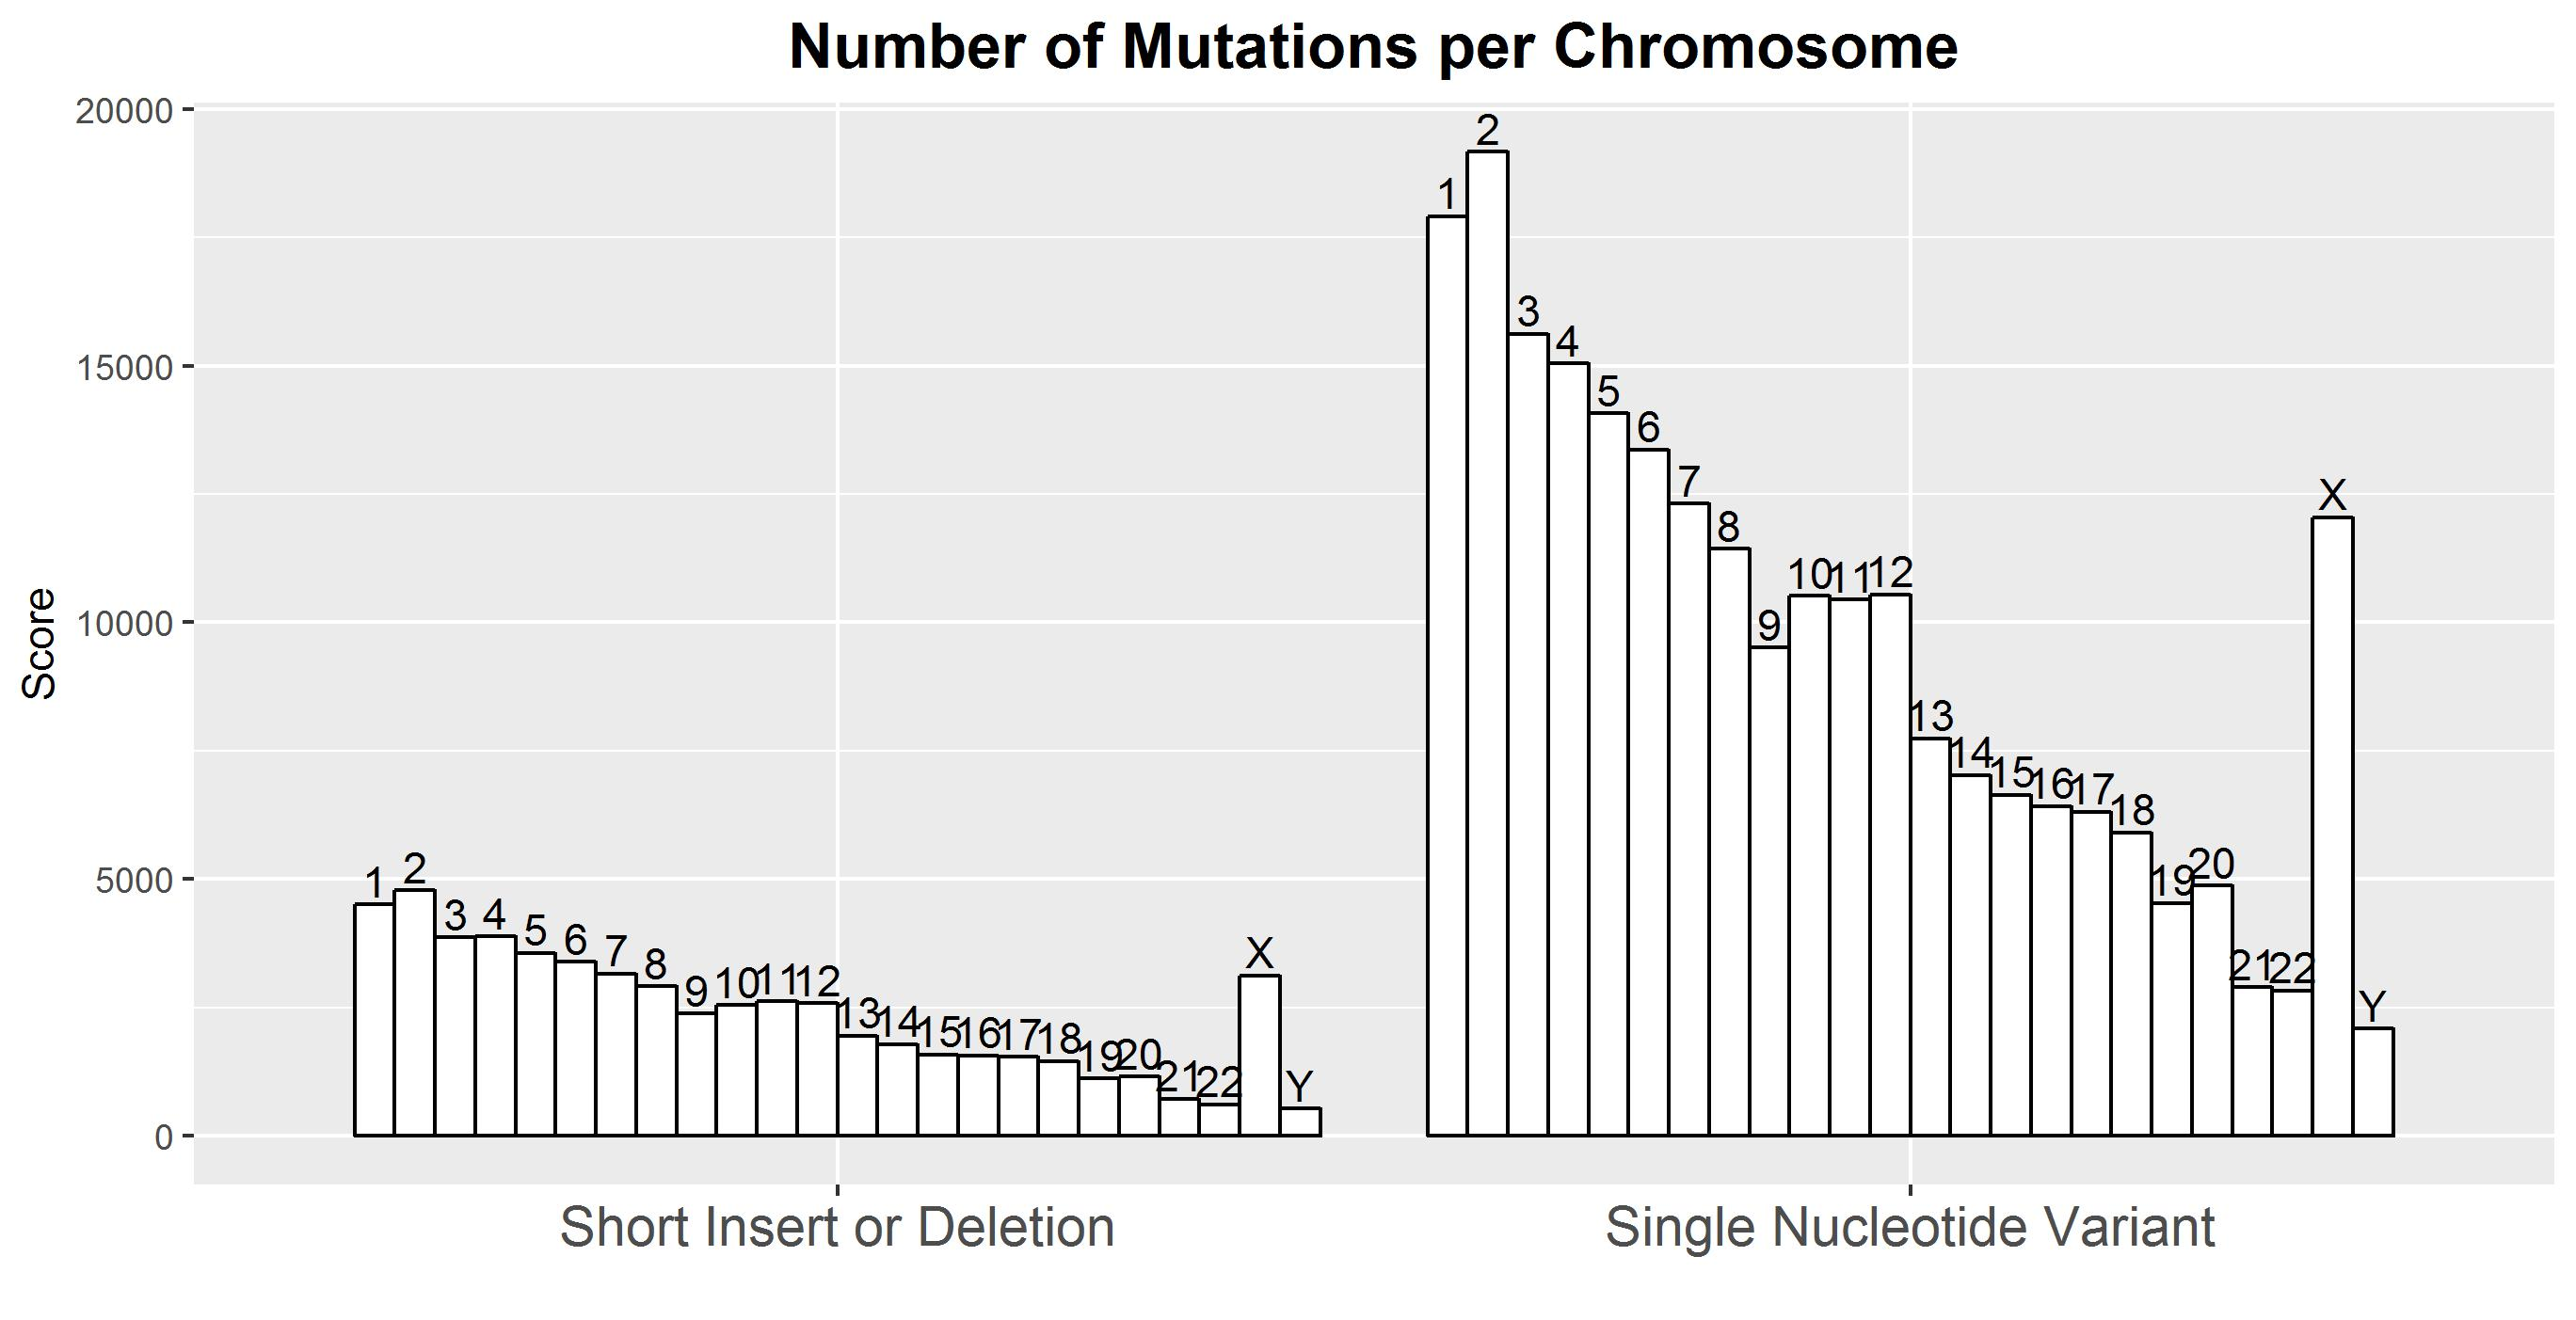
\includegraphics[width=\textwidth]{MutationInSimulatedGenome.jpg}
\caption{Number of ground truth mutations (variants) created in each chromosome }
\end{figure}

\begin{figure}[H]
\centering
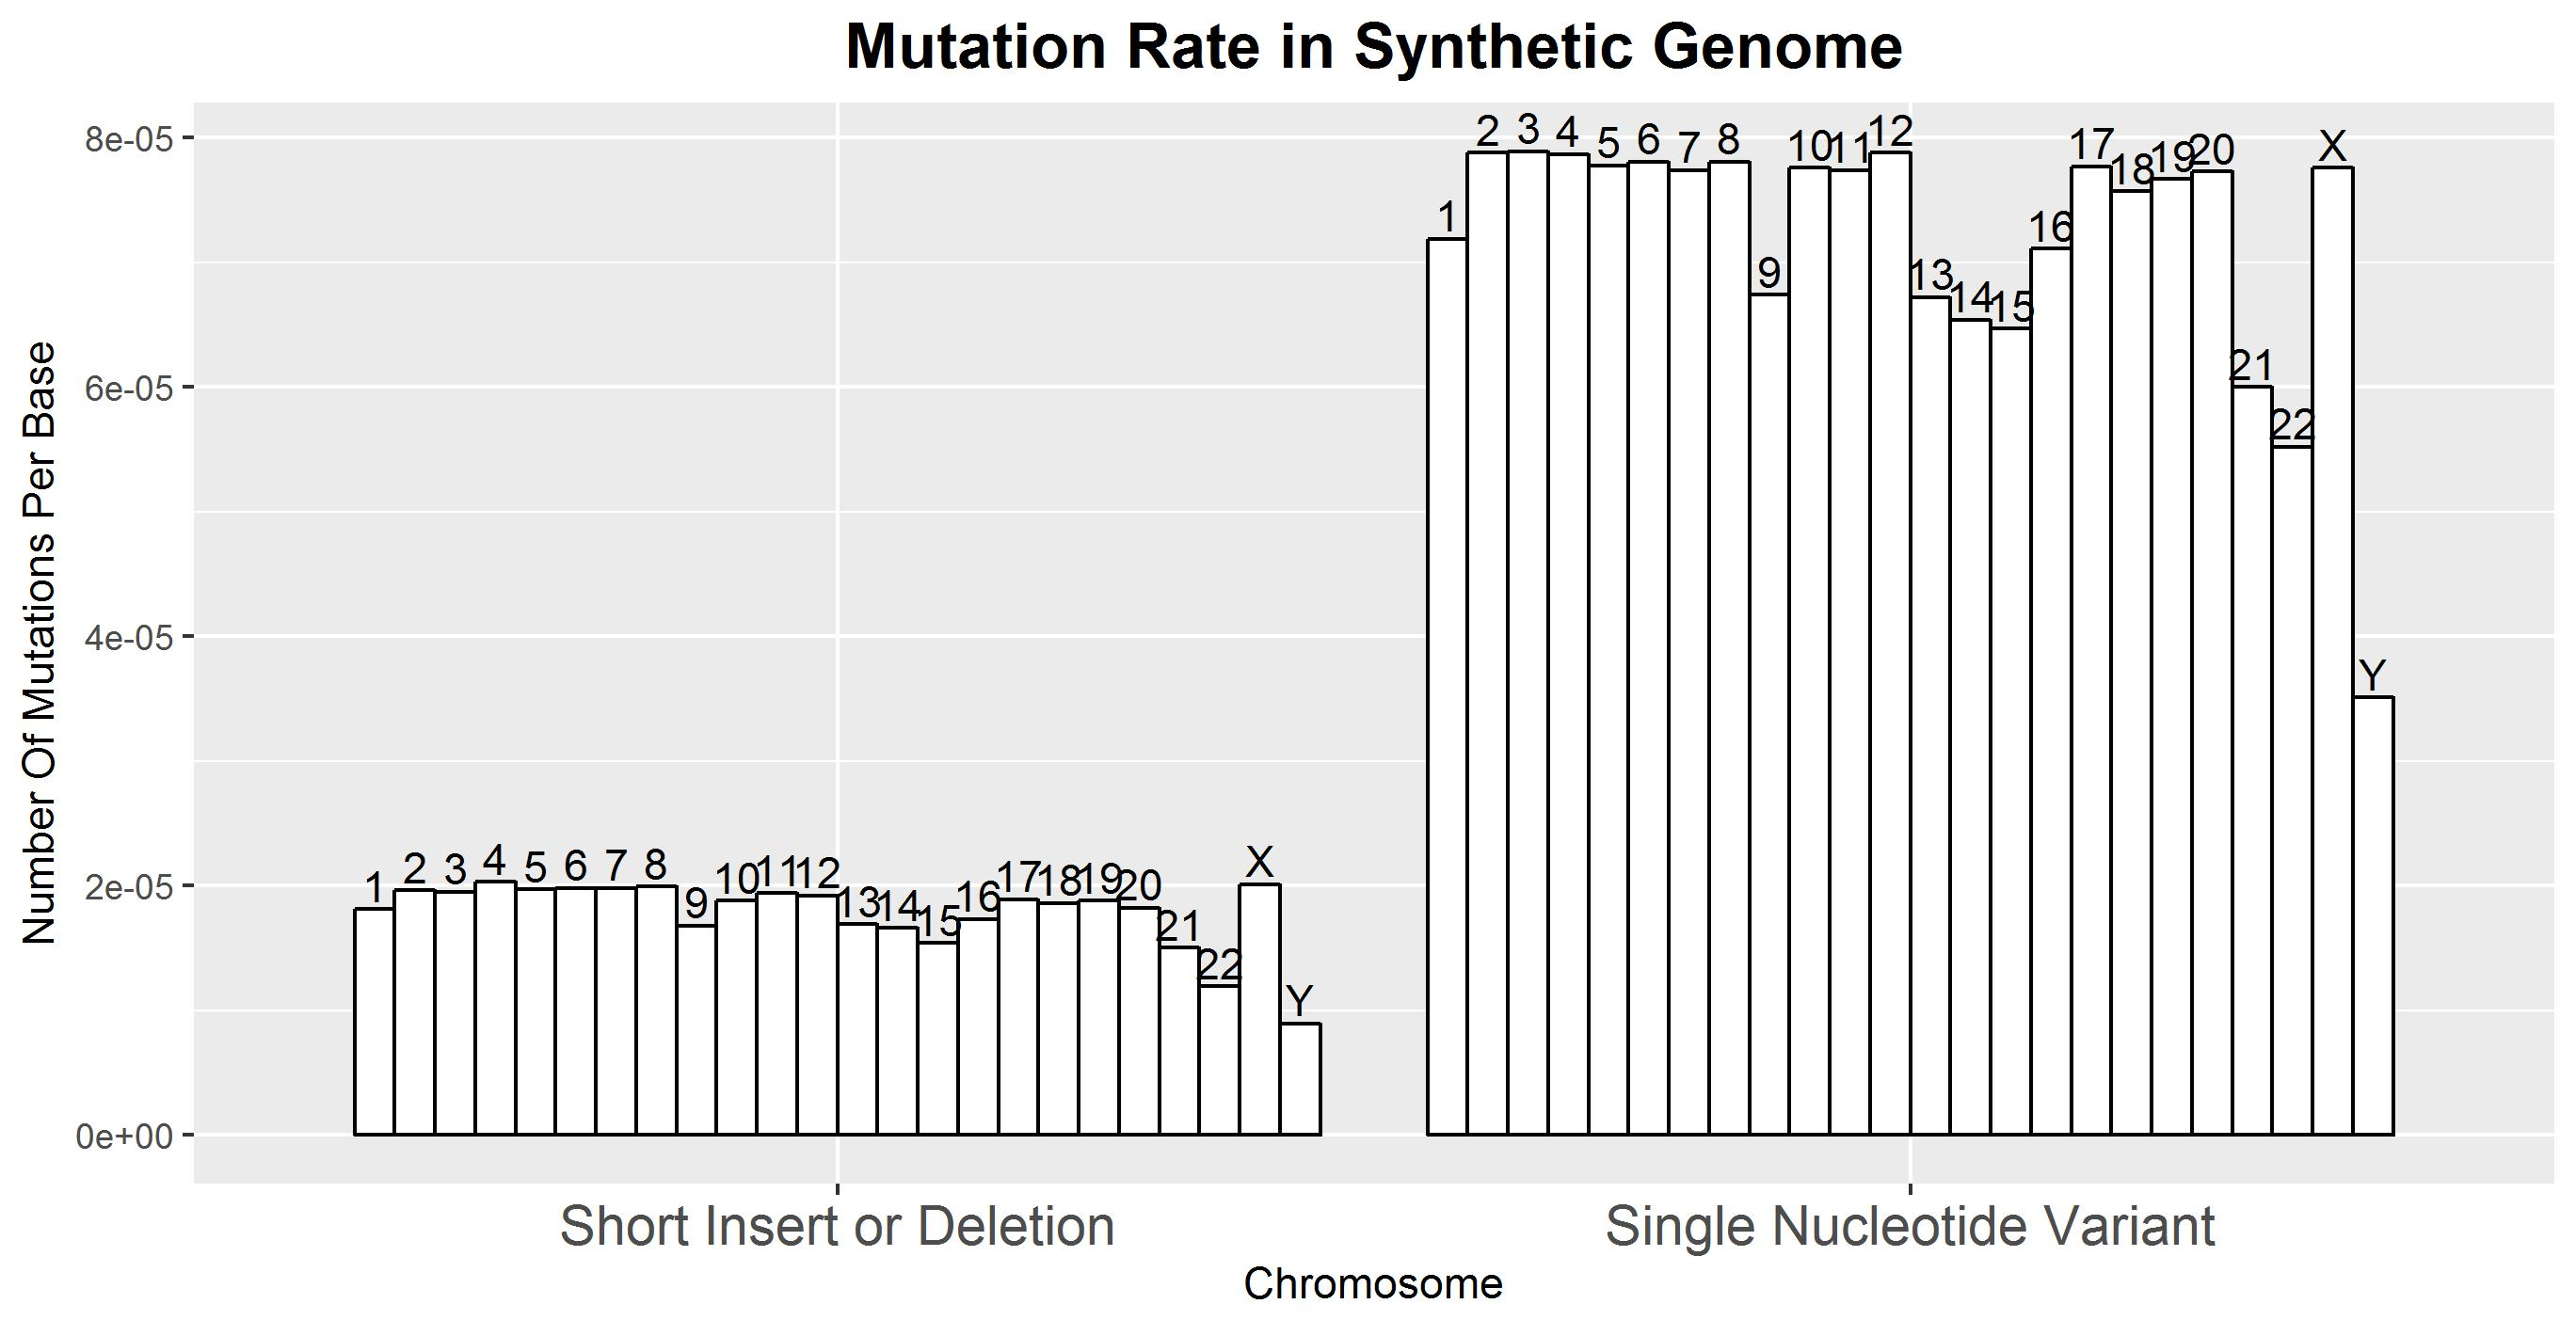
\includegraphics[width=\textwidth]{MutationRateInSimulatedGenome.jpg}
\caption{Mutation rate per base in each chromosome}
\end{figure}

\subsection{Feature Engineering}
Subsequently, we engineered a set of 19 features to use as input data for our variant callers, using data obtained from the variant callers themselves as well as engineering other features from the dataset. A summary of the features used in training can be found in Table 1, and a description of the full list of features can be found in Appendix 5.2. Features were engineered based on obtaining information on the main aspects of variant calling, which includes the information contained in the sample bases (Base Quality, Entropy, Kullback–Leibler divergence, etc.), the confidence we have in the calling and alignment (Read Depth, Mapping Quality etc) and finally possible biases in the sequencing machine (Allele Balance, Allele Count, GC content).

\begin{table}[H]
\caption{Feature Engineering Table}
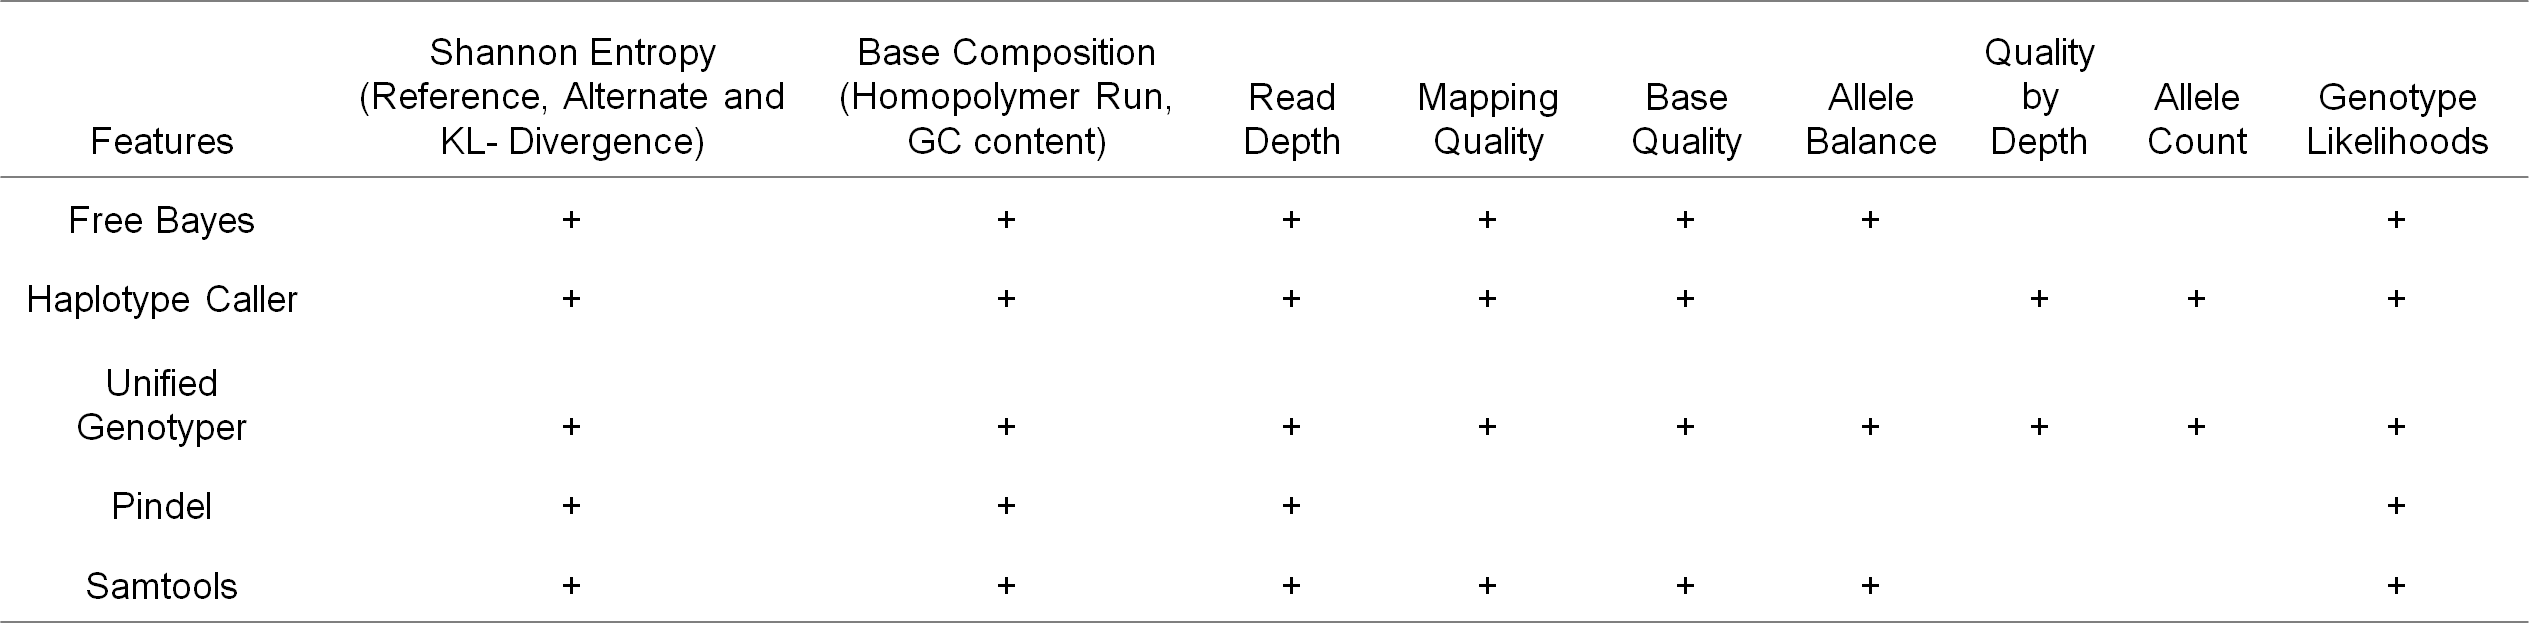
\includegraphics[width=\textwidth]{featureengineering.png}
\centering
\end{table}
\subsection{Variant Callers}
Variant callers were chosen for our deep learning neural network based on their orthogonal calling and reference methodologies - we wanted to optimise the information that the neural network receives (See Table 2). We used two haplotype-based callers, FreeBayes (Garrison \& Marth, 2012) and GATK Haplotype Caller (McKenna et al. 2010, DePristo et al. 2011), two position based callers GATK Unified Genotyper and Samtools (Li H, et al., 2009) and finally Pindel, a pattern growth based caller (Ye et al., 2009). When we analysed the concordance rates of the callers on the simulated dataset, we found a high amount call discordance (Figure 8).
\begin{figure}[H]
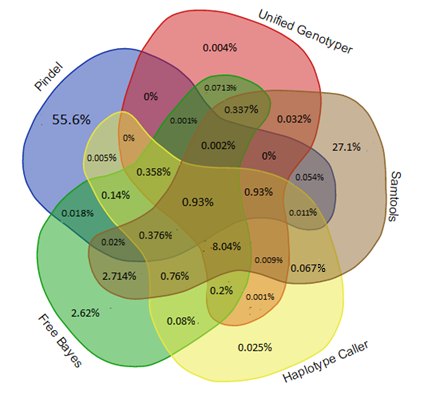
\includegraphics[width=\textwidth]{callconcordances.png}
\centering
\caption{Concordance of callers on simulated dataset, using default settings}
\end{figure} 
Of all the callers, Pindel was the most discordant caller, with over 1.6 million\ (55.6\%) unique calls that are different from other calls. Samtools was also very discordant, with over 800 thousand unique calls (27.1\%) that were unique from the other callers, followed by FreeBayes at 80,000 calls. Interestingly, a high amount of calls (about 100,000) also exists in the intersection of only two callers. Discordance in the variant callers can be explained by the different methodologies that they use to call variants (Table 2). Due to implementation and design choices, as well as statistical methods, each variant caller has a different calling profile. Discordance in the callers provides a strong argument using deep learning to integrate the information from all the callers in a sophisticated manner.

\begin{table}[H]
\caption{Table Comparing Methods and Features of Different variant callers.}
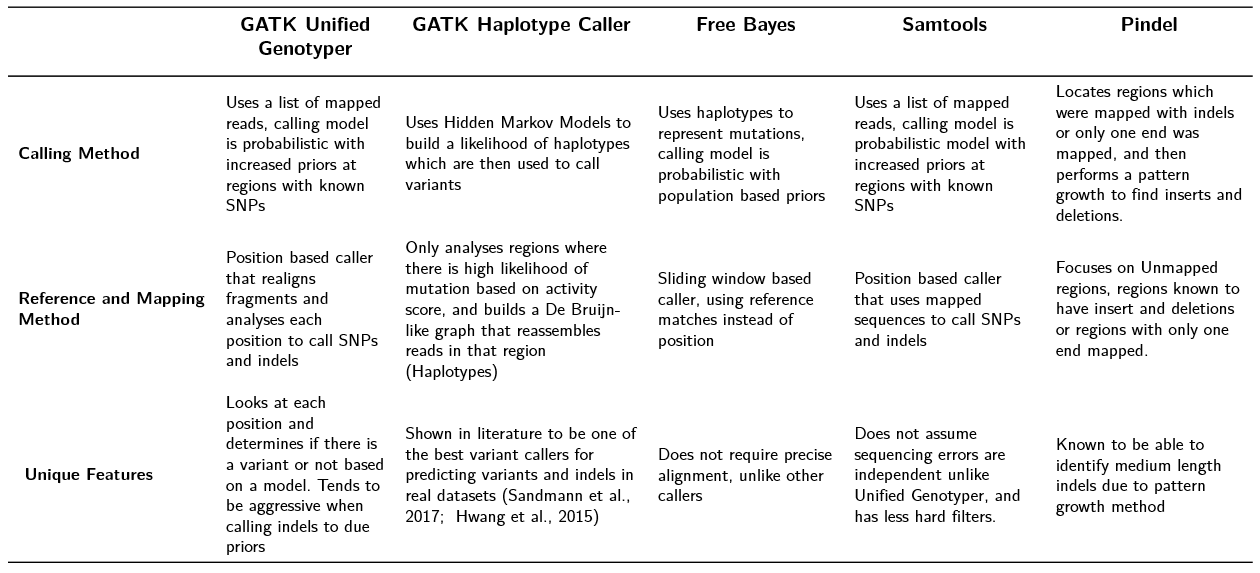
\includegraphics[width=\textwidth]{analysisofvariantcallers.png}
\centering
\end{table}

\subsection{Network Architecture}
Before training our deep learning network, we tested out various neural network architectures to see which architecture would perform the best for our set of input features. We first explored the flat architecture (Figure 10), which contains stacks of fully connected layers with multiple nodes (initially seven layers, with 80 nodes per layer). This is the simplest architecture, where all the features are loaded onto a single vector, and this entire vector is used as an input to train the neural network. We next explored the PCA + flat architecture which had the same neural network architecture but before the input data was fed into the network, a Principal Components Analysis was done to reduce the dataset to 8 principal components which were then used as input data for the neural network (please see Appendix 5.3 for more details of the PCA analysis). Principal components analysis is a dimensionality reduction technique that enables a compressed representation of data. Each principal component is a linear summation of the original features ($X$) in the form 
\begin{align*}
&PC_1 = \beta_{1,1}*X_{1} + \beta_{2,1} X_{2} +... + \beta_{n,1} X_n \\
&... \\
&... \\
&PC_i = \beta_{1,i}*X_{1} + \beta_{2,i} X_{2} +... + \beta_{n,i} X_n
\end{align*}
which enables a few principal components to capture a high amount of variance in the dataset.
Finally, the last architecture we tested was the merged network this network had a set of layers (initially five layers, 24 nodes per layer) that learns from each caller alone, and then the outputs from each of these layers are subsequently merged and used to make a prediction. 
\begin{figure}[H]
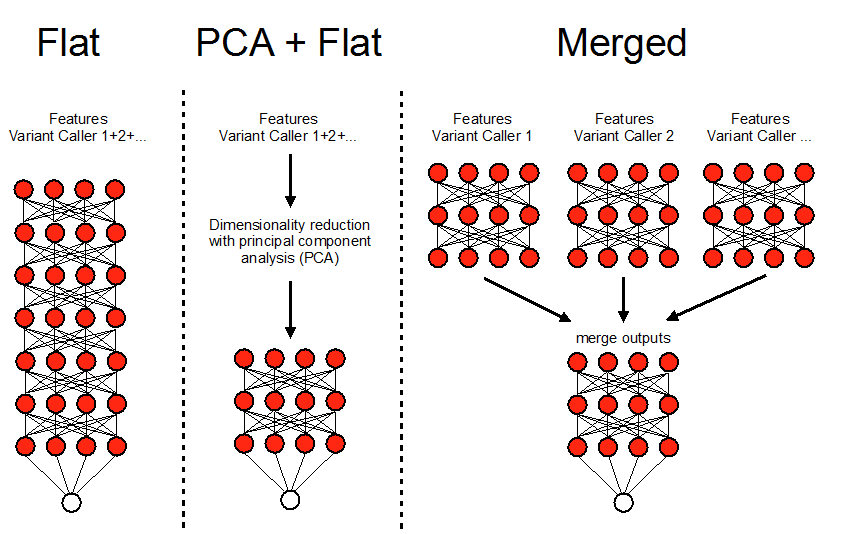
\includegraphics[width=\textwidth]{neuralnetworkstructure.png}
\centering
\caption{Different Designs for Neural Network Architecture}
\end{figure}
To study how well each architecture is able to perform, we use the metrics of precision, recall and F1 score. Precision measures how many mistakes the predictor makes (the ratio of true positives over false positives and true positives), recall measures what portion of the truth class a predictor can discover (the ratio of true positives over true positives and false negatives) and finally the F1 score is composite function of both precision and recall. The derivations of the metrics can be found in Appendix 5.3.1. 
\begin{figure}[H]
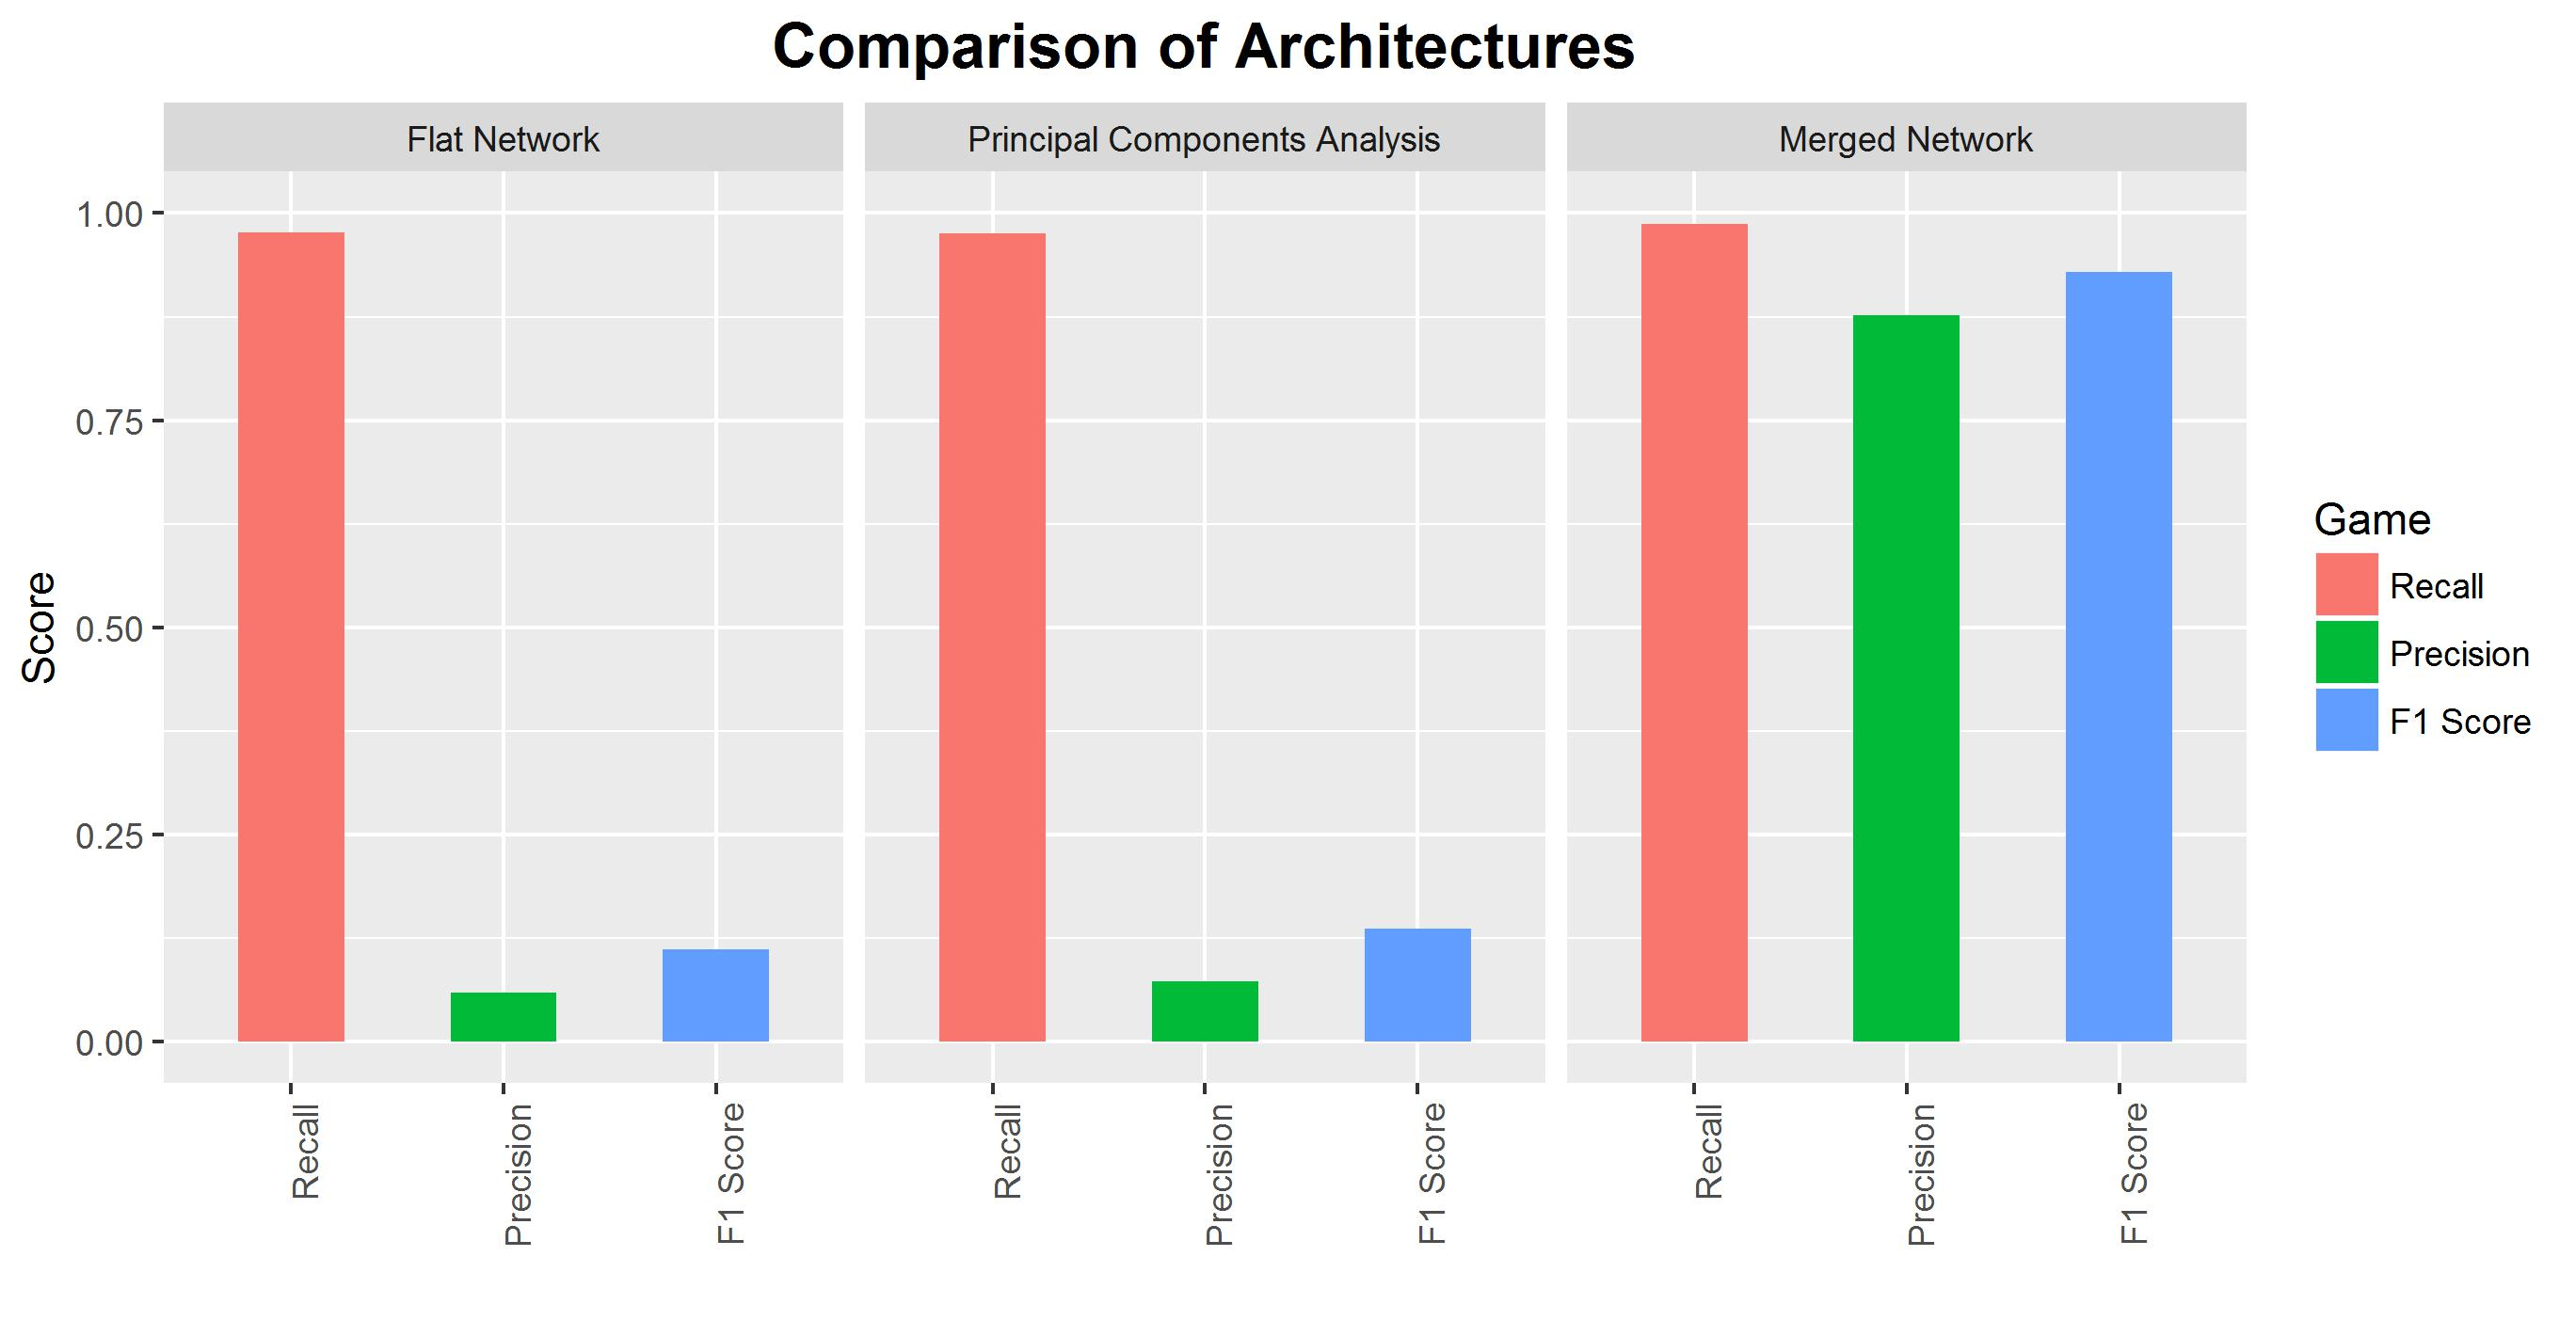
\includegraphics[width=\textwidth]{neuralnetworkstructureresults.jpg}
\centering
\caption{Analysis of Different Neural Network Architecture}
\end{figure}
Initially, with the flat network, the precision rate was very low at 0.059 with an F1 score of 0.112, indicating that the neural network was unable to learn from the input feature set. We suspected that this was due to high dimensionality in the dataset, which led to our second architecture design, the PCA with flat analysis. Principal components analysis has been shown to be able to successfully improve learning in high-dimensionality datasets (Chen et al., 2014; Van Der Maaten, Postma \& Van den Herik, 2009). However, the precision and F1 score for the PCA architecture was also low at 0.0735 and 0.137 respectively. Ultimately both failed to learn, indicating to us that perhaps the features from each of the callers had to be analysed separately before being passed into a separate neural network that did the final output integration. With this merged network, we managed to obtain a precision score(0.877) and an F1 score(0.929) that was far better than the previous two architectures. Interestingly, the recall scores for all three architectures were around the same ($\pm 0.01$), indicating the main difference for the neural network was in its ability to remove false positive calls.

\subsection{Network Tuning and Optimisation}
Next, we systematically optimised and tuned the deep learning neural network to maximise its predictive ability. In tuning our network, we also sought to study how the various hyperparameters as well as the data structure affected our network's ability to learn from the data. In particular, we focused on four issues - the number of layers, optimiser choice, learning rate choice and finally sample balancing. These four issues are known to be critical in deep learning networks (Ruder et al., 2016; LeCun, Bengio \& Hinton, 2015; Yan et al., 2015;  Sutskever et al., 2013) and would likely be critical to the success of a deep learning neural network.\\\\
\subsubsection{Number of Layers}
Firstly, we studied how many layers should be in the neural network. The number of layers is critical as it determines what kind of information and the representation of data that can be captured by the neural network. Choosing the number of layers is important as sufficient layers are needed to obtain the complex data representation needed for learning, but too many layers might result in the vanishing gradient problem. We started off with a neural network architecture as shown below, and began to vary the number of layers in at each point.
\begin{figure}[H]
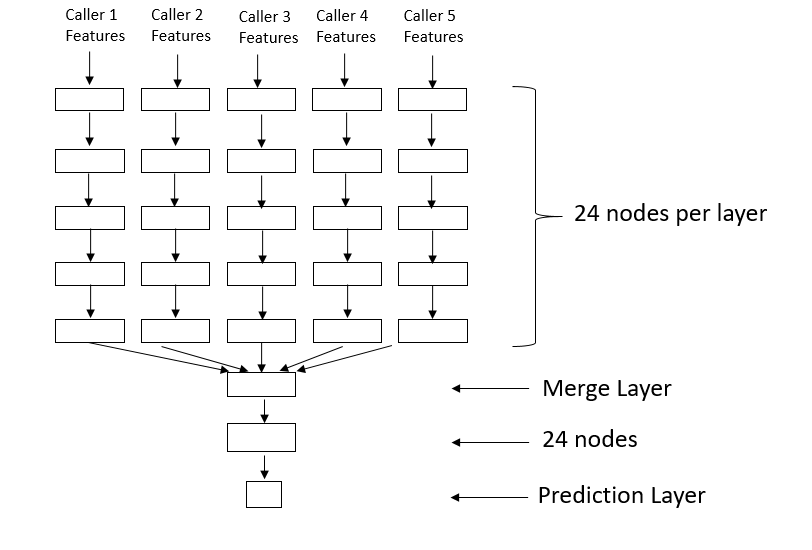
\includegraphics[width=\textwidth]{neuralnetworkarchitecturefinal.png}
\centering
\caption{Basic Merge Network Structure}
\end{figure}
For all layers, the LeakyReLU activation function was used. The LeakyReLU is a refinement of the ReLU activation function which minimises the "dying ReLU" problem, and both are well-documented activation functions that have been shown to work well in deep neural networks (Anthimopoulos et al., 2016; LeCun, Bengio \& Hinton, 2015; Maas, Hannun \& Ng, 2013). We noticed that changing the number of layers after the merge layer did not significantly vary the output, and so we focused on changing the number of layers before the merge layer. We studied 6 different neural network structures (4 layers to 9 layers). 
\begin{figure}[H]
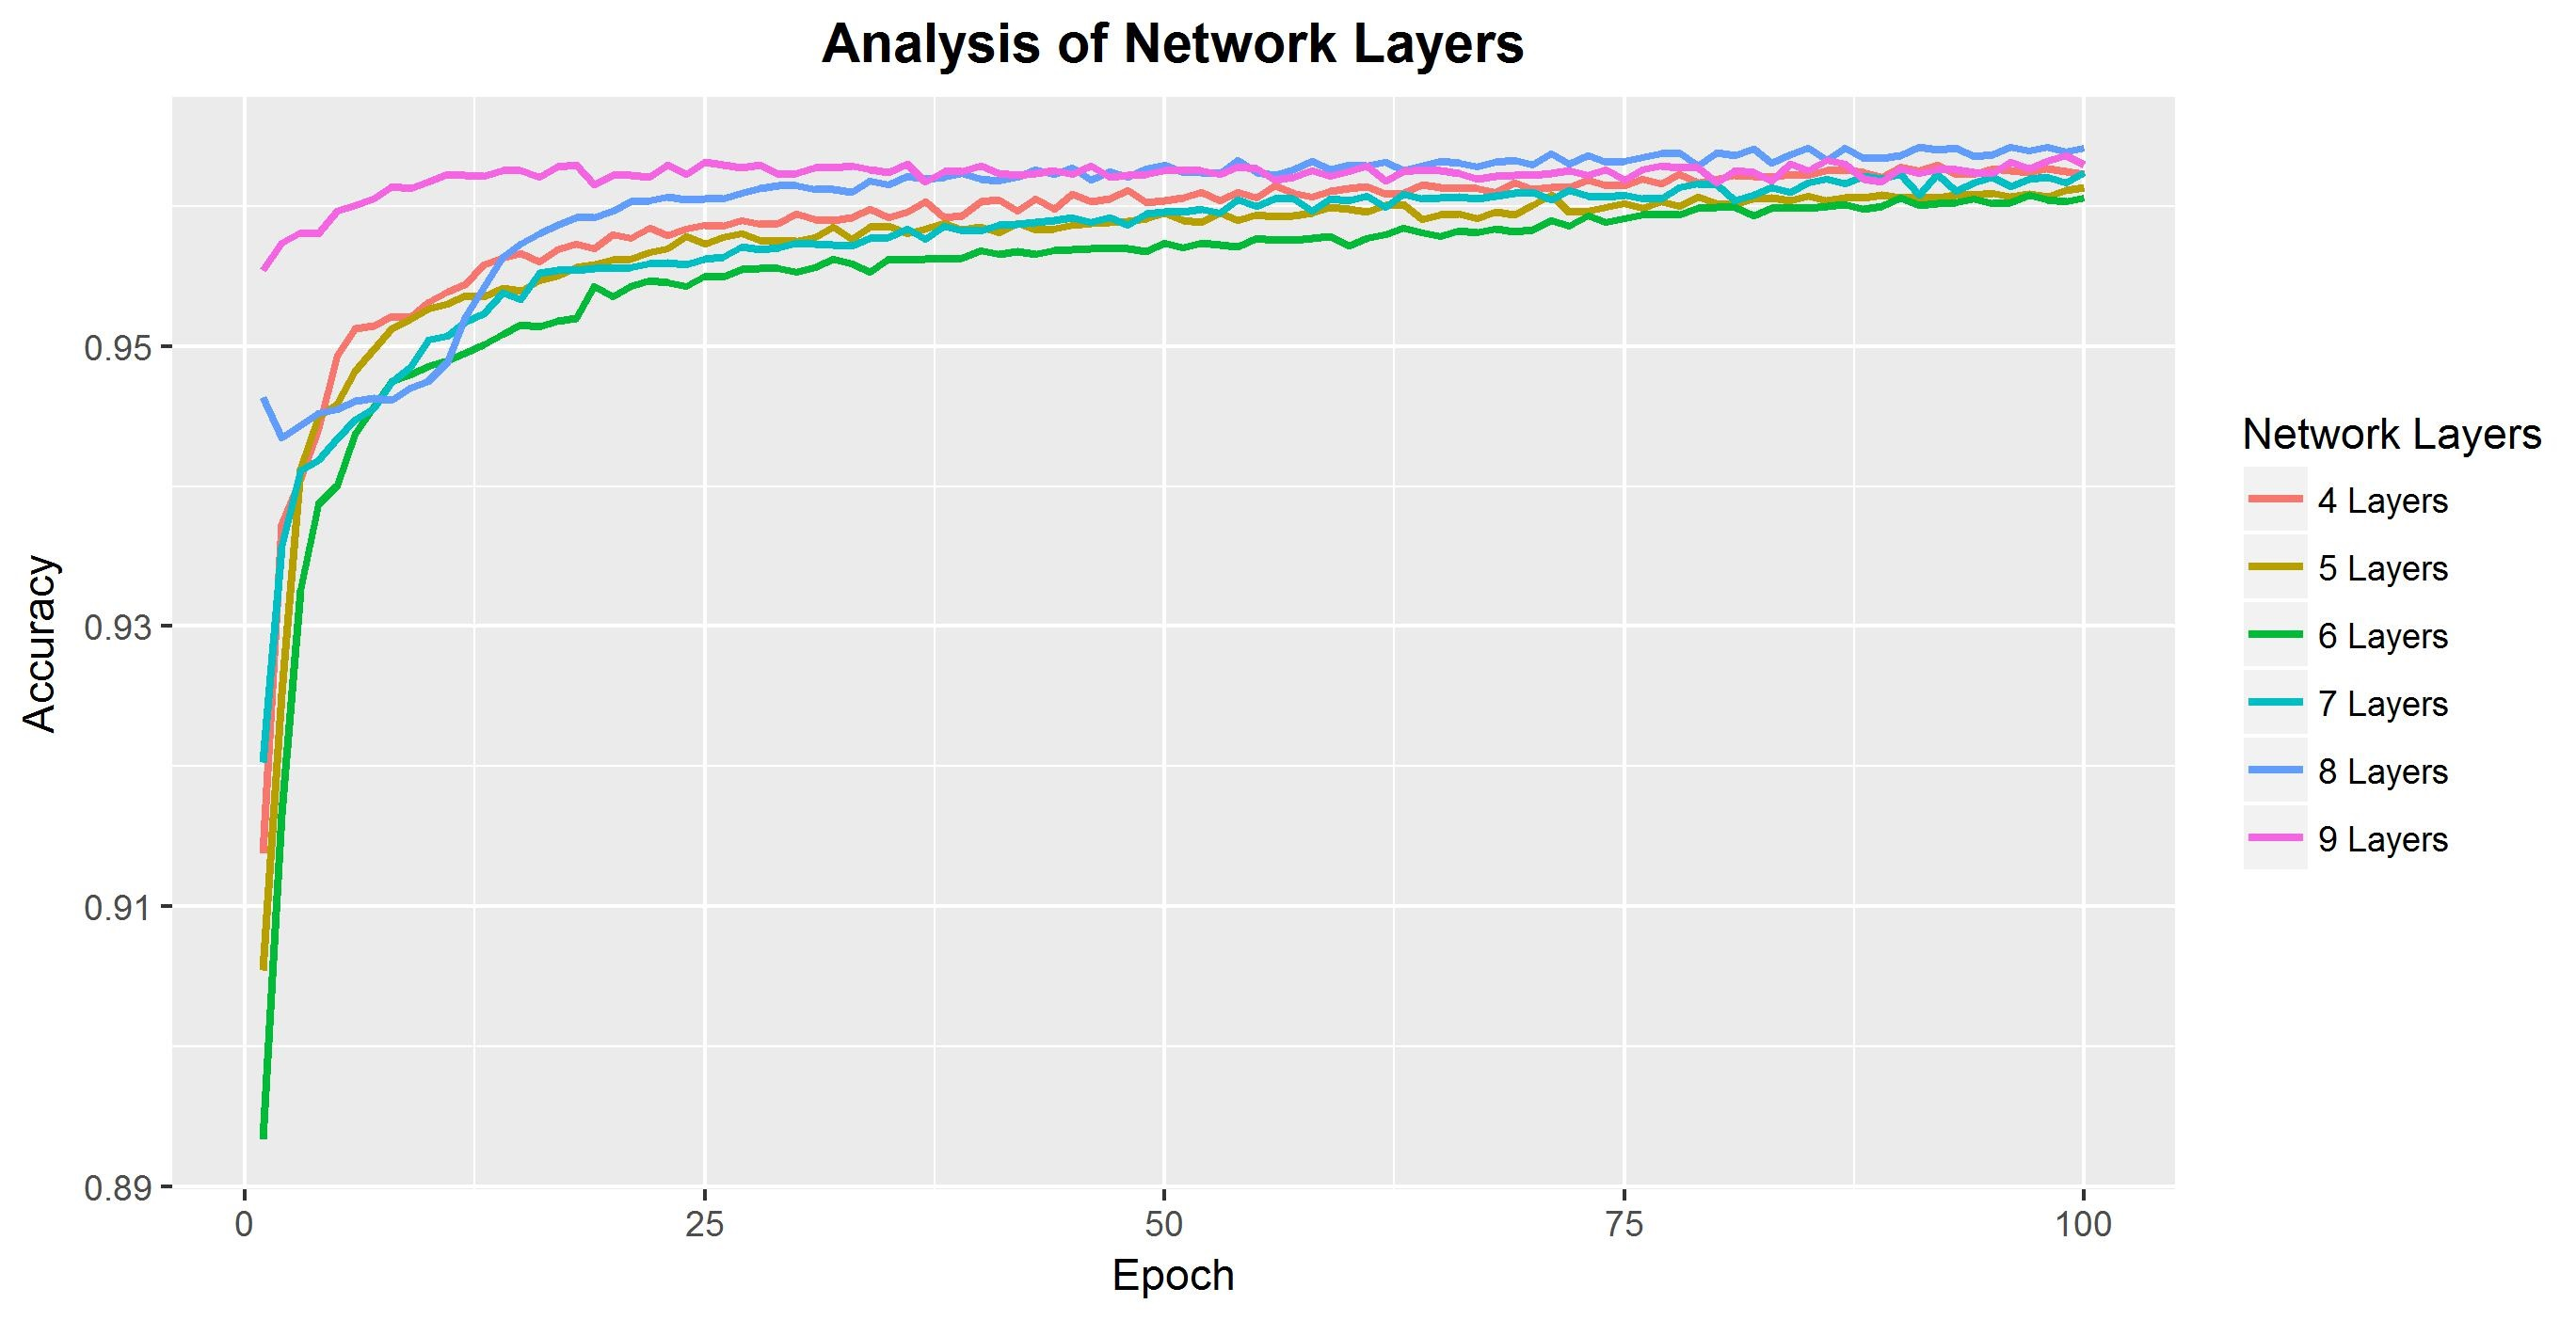
\includegraphics[width=\textwidth]{networkstructuredataset.jpg}
\centering
\caption{Analysis of Different Number of Layers On Training Accuracy}
\end{figure}
From analysing the accuracies of the different layers, we find that 8 layers seem the best at learning from the input data. We note that all the layers follow the same rough trend of accuracy, indicating they are all able to learn from the dataset. We decided on the 8 layer network as it seemed best able to learn from the input dataset, with a final accuracy of 0.964 that is about 0.001 higher than other layers. A final design feature used was to add two dropout filters at the last two layers before merging in order to prevent overfitting in data. Dropout filters have been shown to be an effective in preventing overfitting of data (Srivastava et al., 2014). Another active step taken to prevent overfitting was to ensure random separation of test, validation and training datasets.\\\\
\subsubsection{Optimiser and Learning Rates}
Next, we sought to choose the best optimiser and learning rate for our dataset. Both optimisers and learning rates have been well studied and known to be important in neural network training (Ruder et al., 2016; Sutskever et al., 2013). Optimiser choice is critical as the optimisers determine how the weights and gradients are updated in the network, thus playing an integral part in learning. We studied 3 well-known optimisers for use in our network, ADAM, RMSprop and Stochastic Gradient Descent (SGD). ADAM is an adaptive learning rate optimiser that is known to be well suited in large dataset and parameter problems(Kingma \& Ba, 2014). RMSprop is another adaptive learning rate optimiser that unpublished, but has been shown to work well for real experimental datasets (Tieleman \& Hinton, 2012). SGD is the simplest learning model with no adaptive learning rate but is a useful model because it is the easiest to understand mathematically and has also been shown to solve deep learning problems (Kingma \& Ba, 2014). For more information on the mathematical foundations of optimisation and backpropagation, please see Appendix 5.1. For the three optimisers, we ran tests to study the accuracy of the neural network running on each optimiser to predict true variants (Figure 11).
\begin{figure}[H]
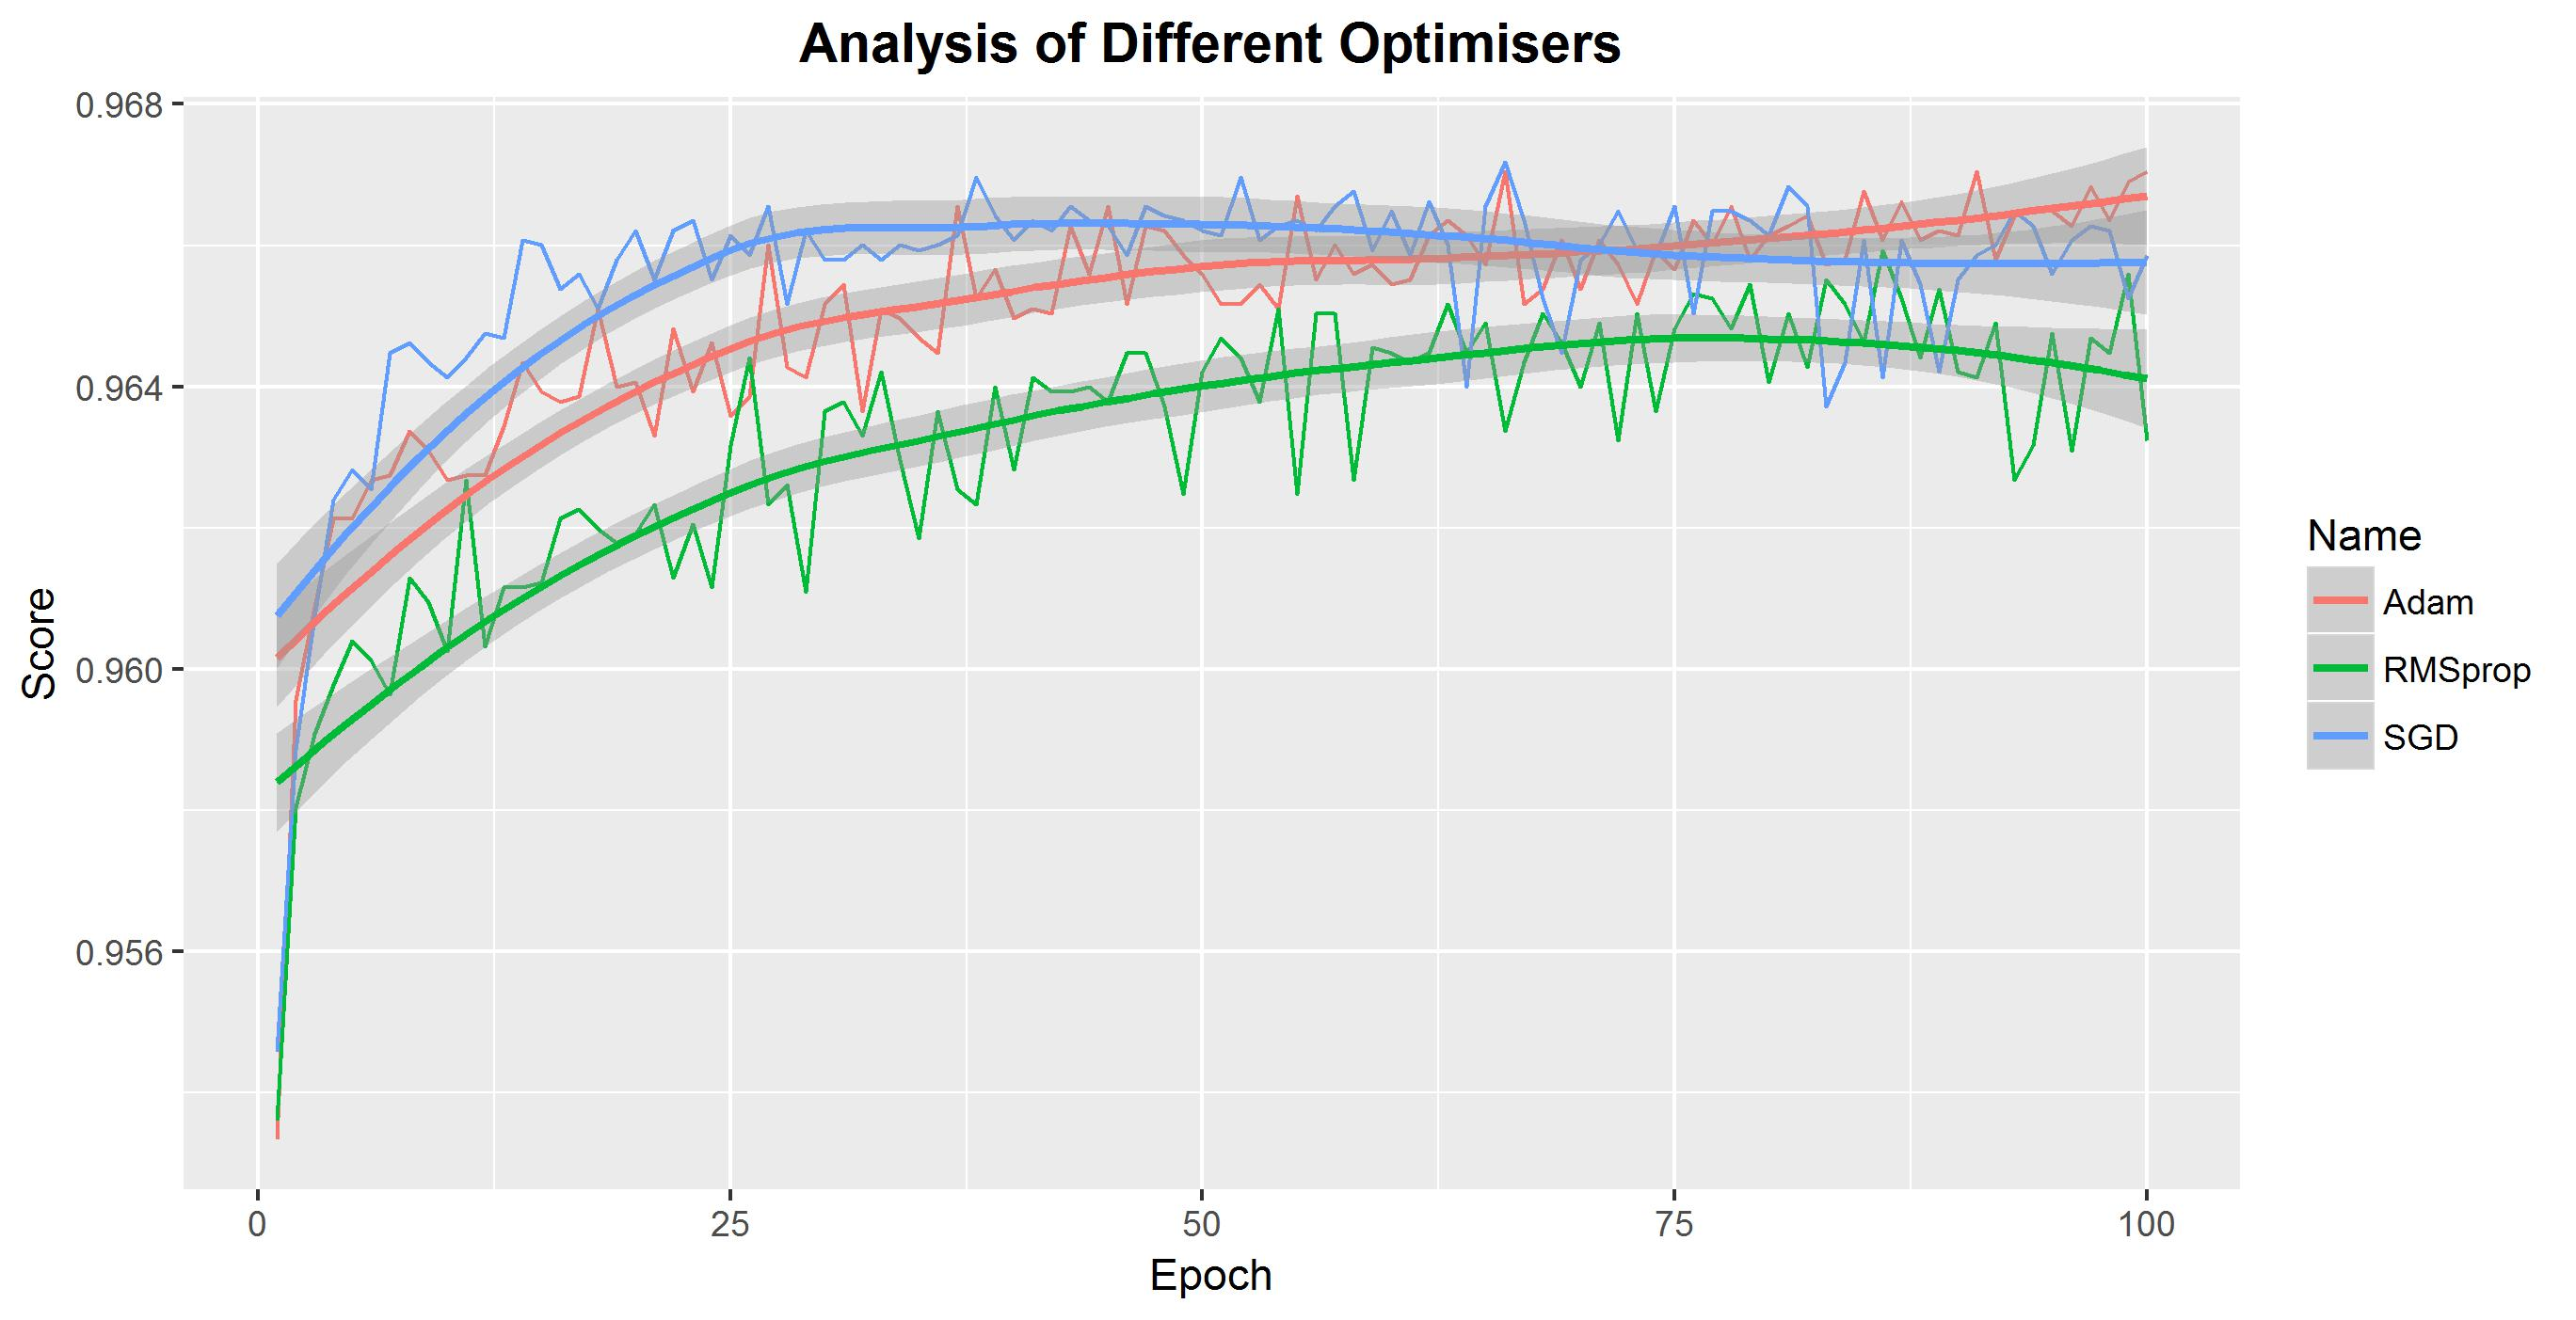
\includegraphics[width=\textwidth]{optimiserlearning.jpg}
\centering
\caption{Optimiser accuracies for training at each epoch. Due to the noise in accuracies, the overall momentum of the dataset, calculated as a sliding window average is shown. The 95\% confidence interval is also shown.}
\end{figure}
The adaptive rate optimisers, Adam and RMSprop obtained the highest accuracies of 0.9670 and 0.9660 while SGD reached a maximum accuracy of 0.9569, very close to that of RMSprop. Interestingly adaptive rate optimisers seemed to have complex learning trajectories, while SGD has a very stable learning rate. This makes sense as adaptive learning rates allow greater gradient descents when the error is high, and decreasing the learning rate at smaller errors (Kingma and Ba, 2014; Zeiler, 2012). This allows Adam and RMSprop to learn at variable rates based on the current gradients. For SGD, it appears that while it takes a while to learn the true minima, it eventually still reaches about the same minima as RMSprop. Ultimately, we chose Adam as our optimiser as the final accuracy discovered by Adam was noted to be higher than RMSprop and SGD, and we note a stable learning curve for Adam, indicating it is able to learn and update the gradients in the neural network to learn from input data at all epochs. Subsequently, we also looked at various initial learning rate for Adam (Figure 12) and found that the most stable learning could be found at a learning rate of $10^{-5}$. This initial learning rate is critical as it determines the first few gradient descents which enable stable adaptive learning throughout the epochs (Sutskever et al., 2013). At any larger learning rates ($10^{-4}$ and below), a very high amount of noise was observed, indicating that the learning rate was too high resulting in minima finding errors. At smaller learning rates ($10^{-6}$ and above), the final accuracy after 100 epochs (0.9639 for $10^{-6}$) was lower than the learning rate at $10^{-5}$ (0.9672). Thus, we chose $10^{-5}$ to be our learning rate.
\begin{figure}[H]
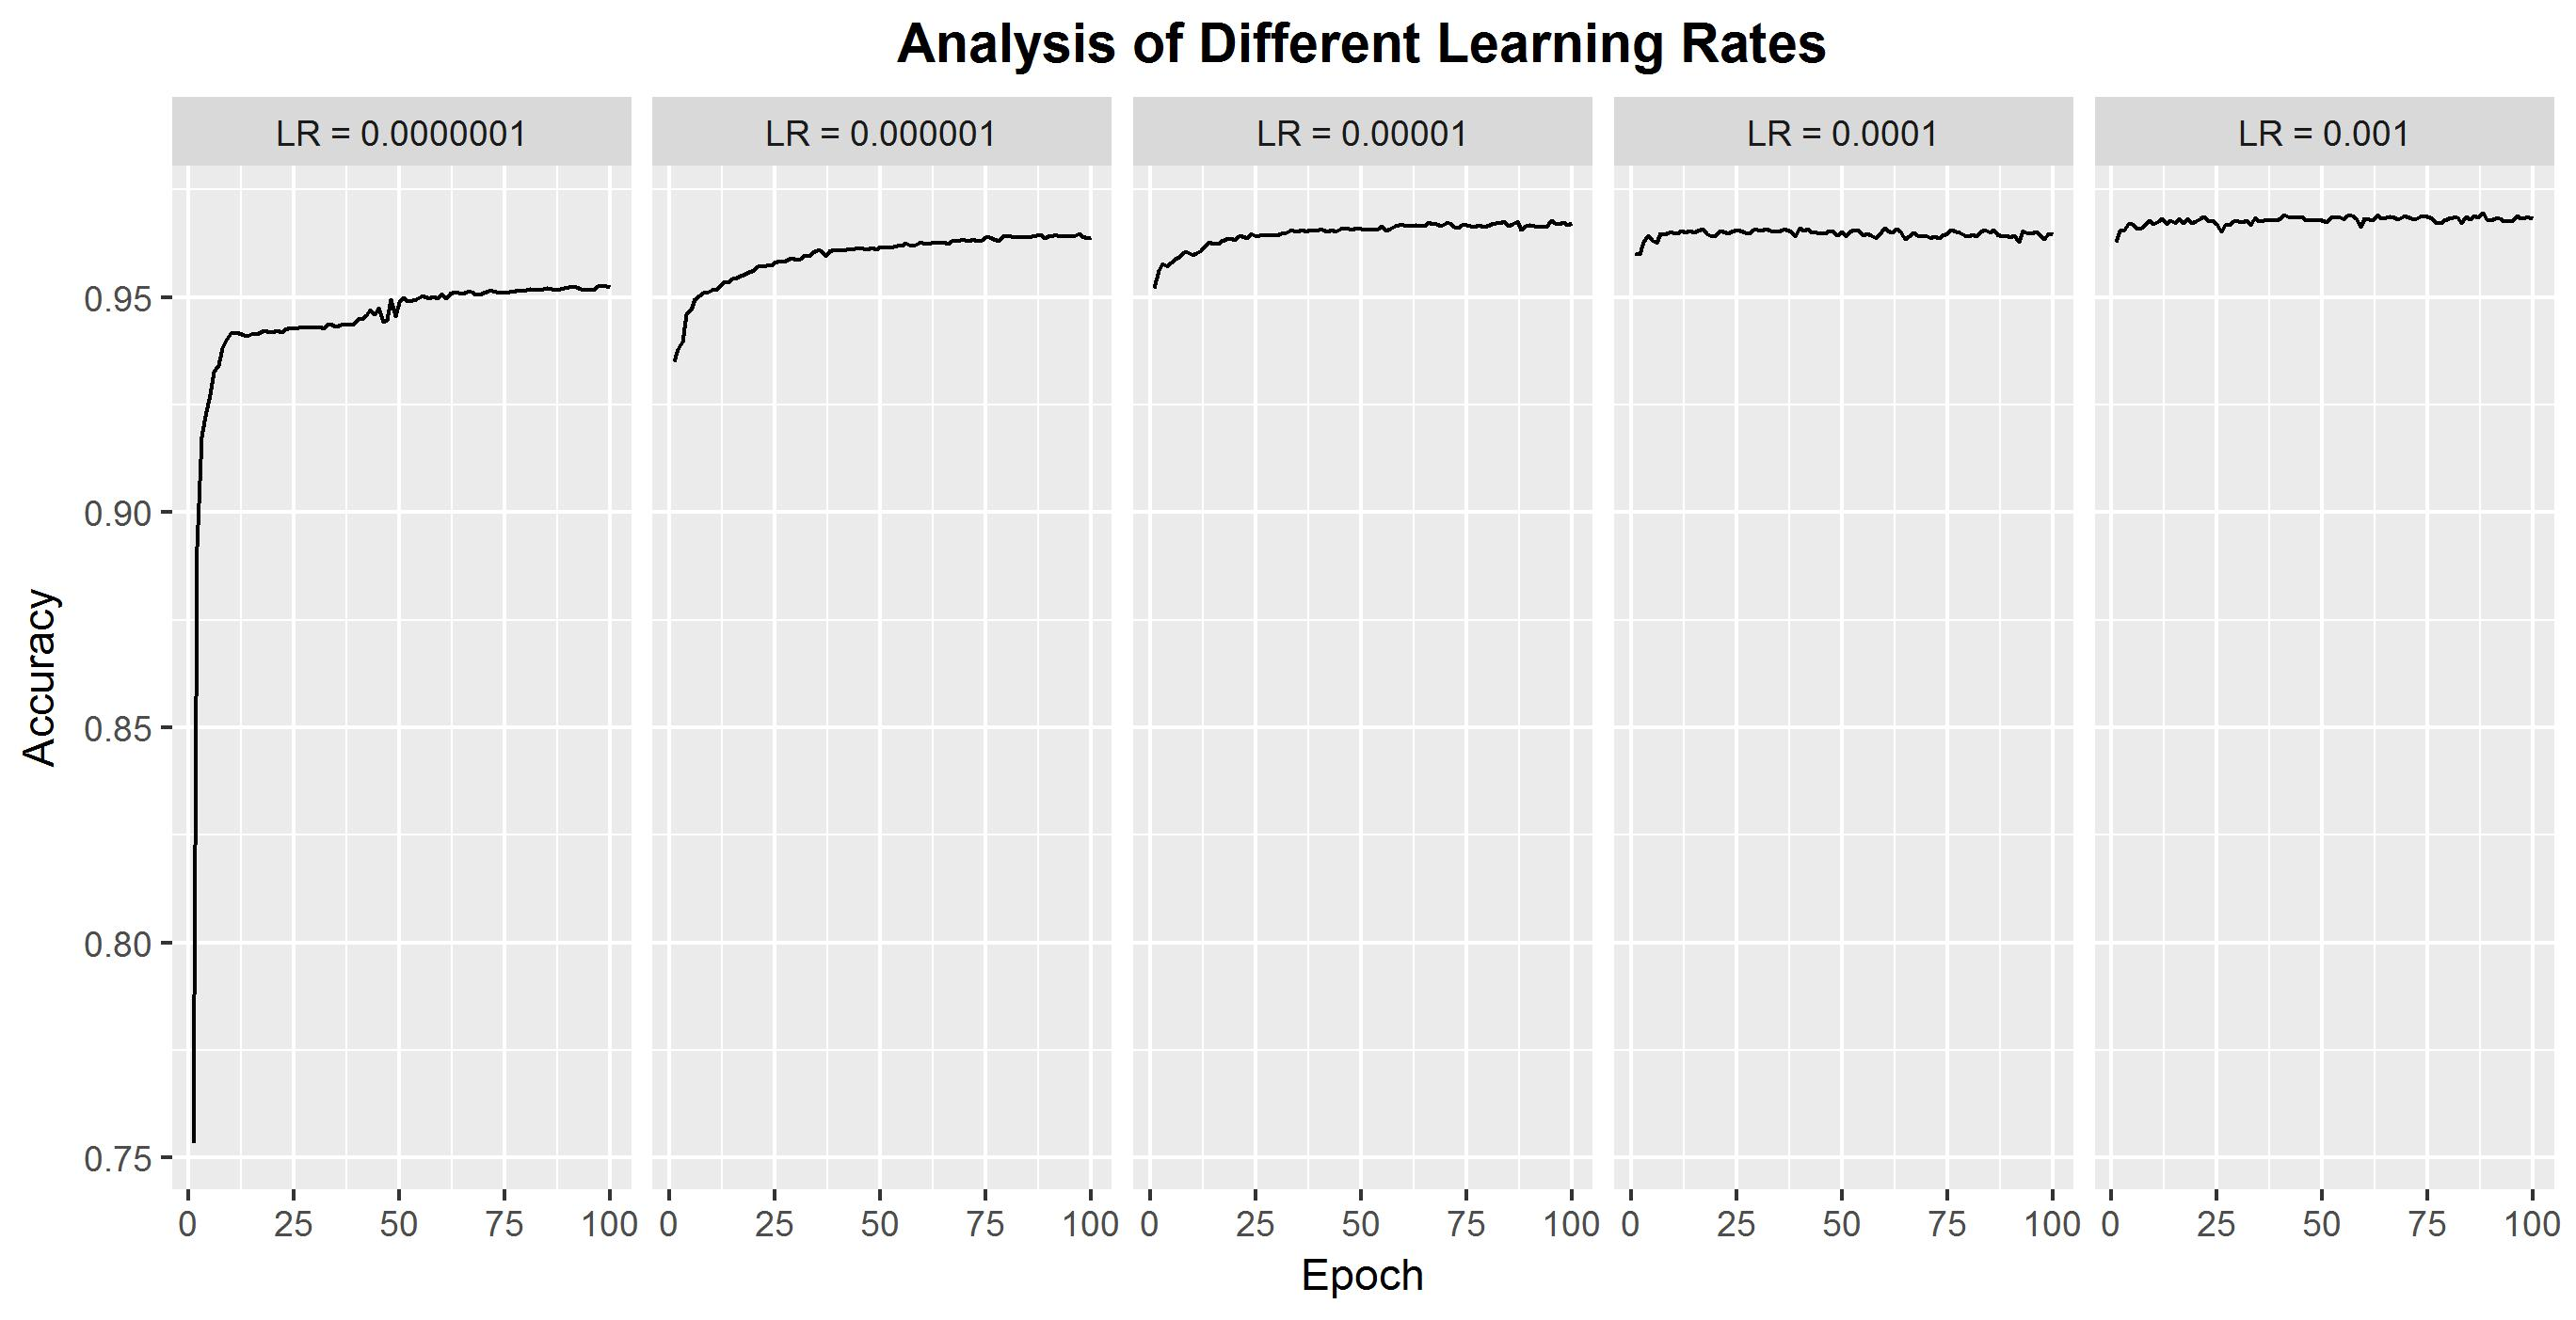
\includegraphics[width=\textwidth]{learningrates.jpg}
\centering
\caption{Training Accuracies over Each Epoch for Different Learning Rates}
\end{figure}
\subsubsection{Sample Balancing}
Our final concern was sample balancing - the simulated dataset contained an imbalance of positive training examples versus negative training examples. In total, there were 286569 positive training examples and 4547919 negative training examples, which is a 15-fold difference. Such a sample imbalance has been known to affect learning adversely (Yan et al., 2015; López et al., 2012). Thus, we sought to implement two methods of sample balancing, undersampling and oversampling. Undersampling was implemented by removing negative training examples until the number of negative training examples was equal to the number of positive training examples. In oversampling, the Synthetic Minority Oversampling Technique(SMOTE) was done, which uses nearest neighbours to create more data points for the positive training example. Specifically, SMOTE looks at two nearby positive class examples, and creates a new synthetic example in the middle of these two examples (see Appendix 5.3 for more details). Figure 13 shows the metrics for each sampling technique.
\begin{figure}[H]
\centering
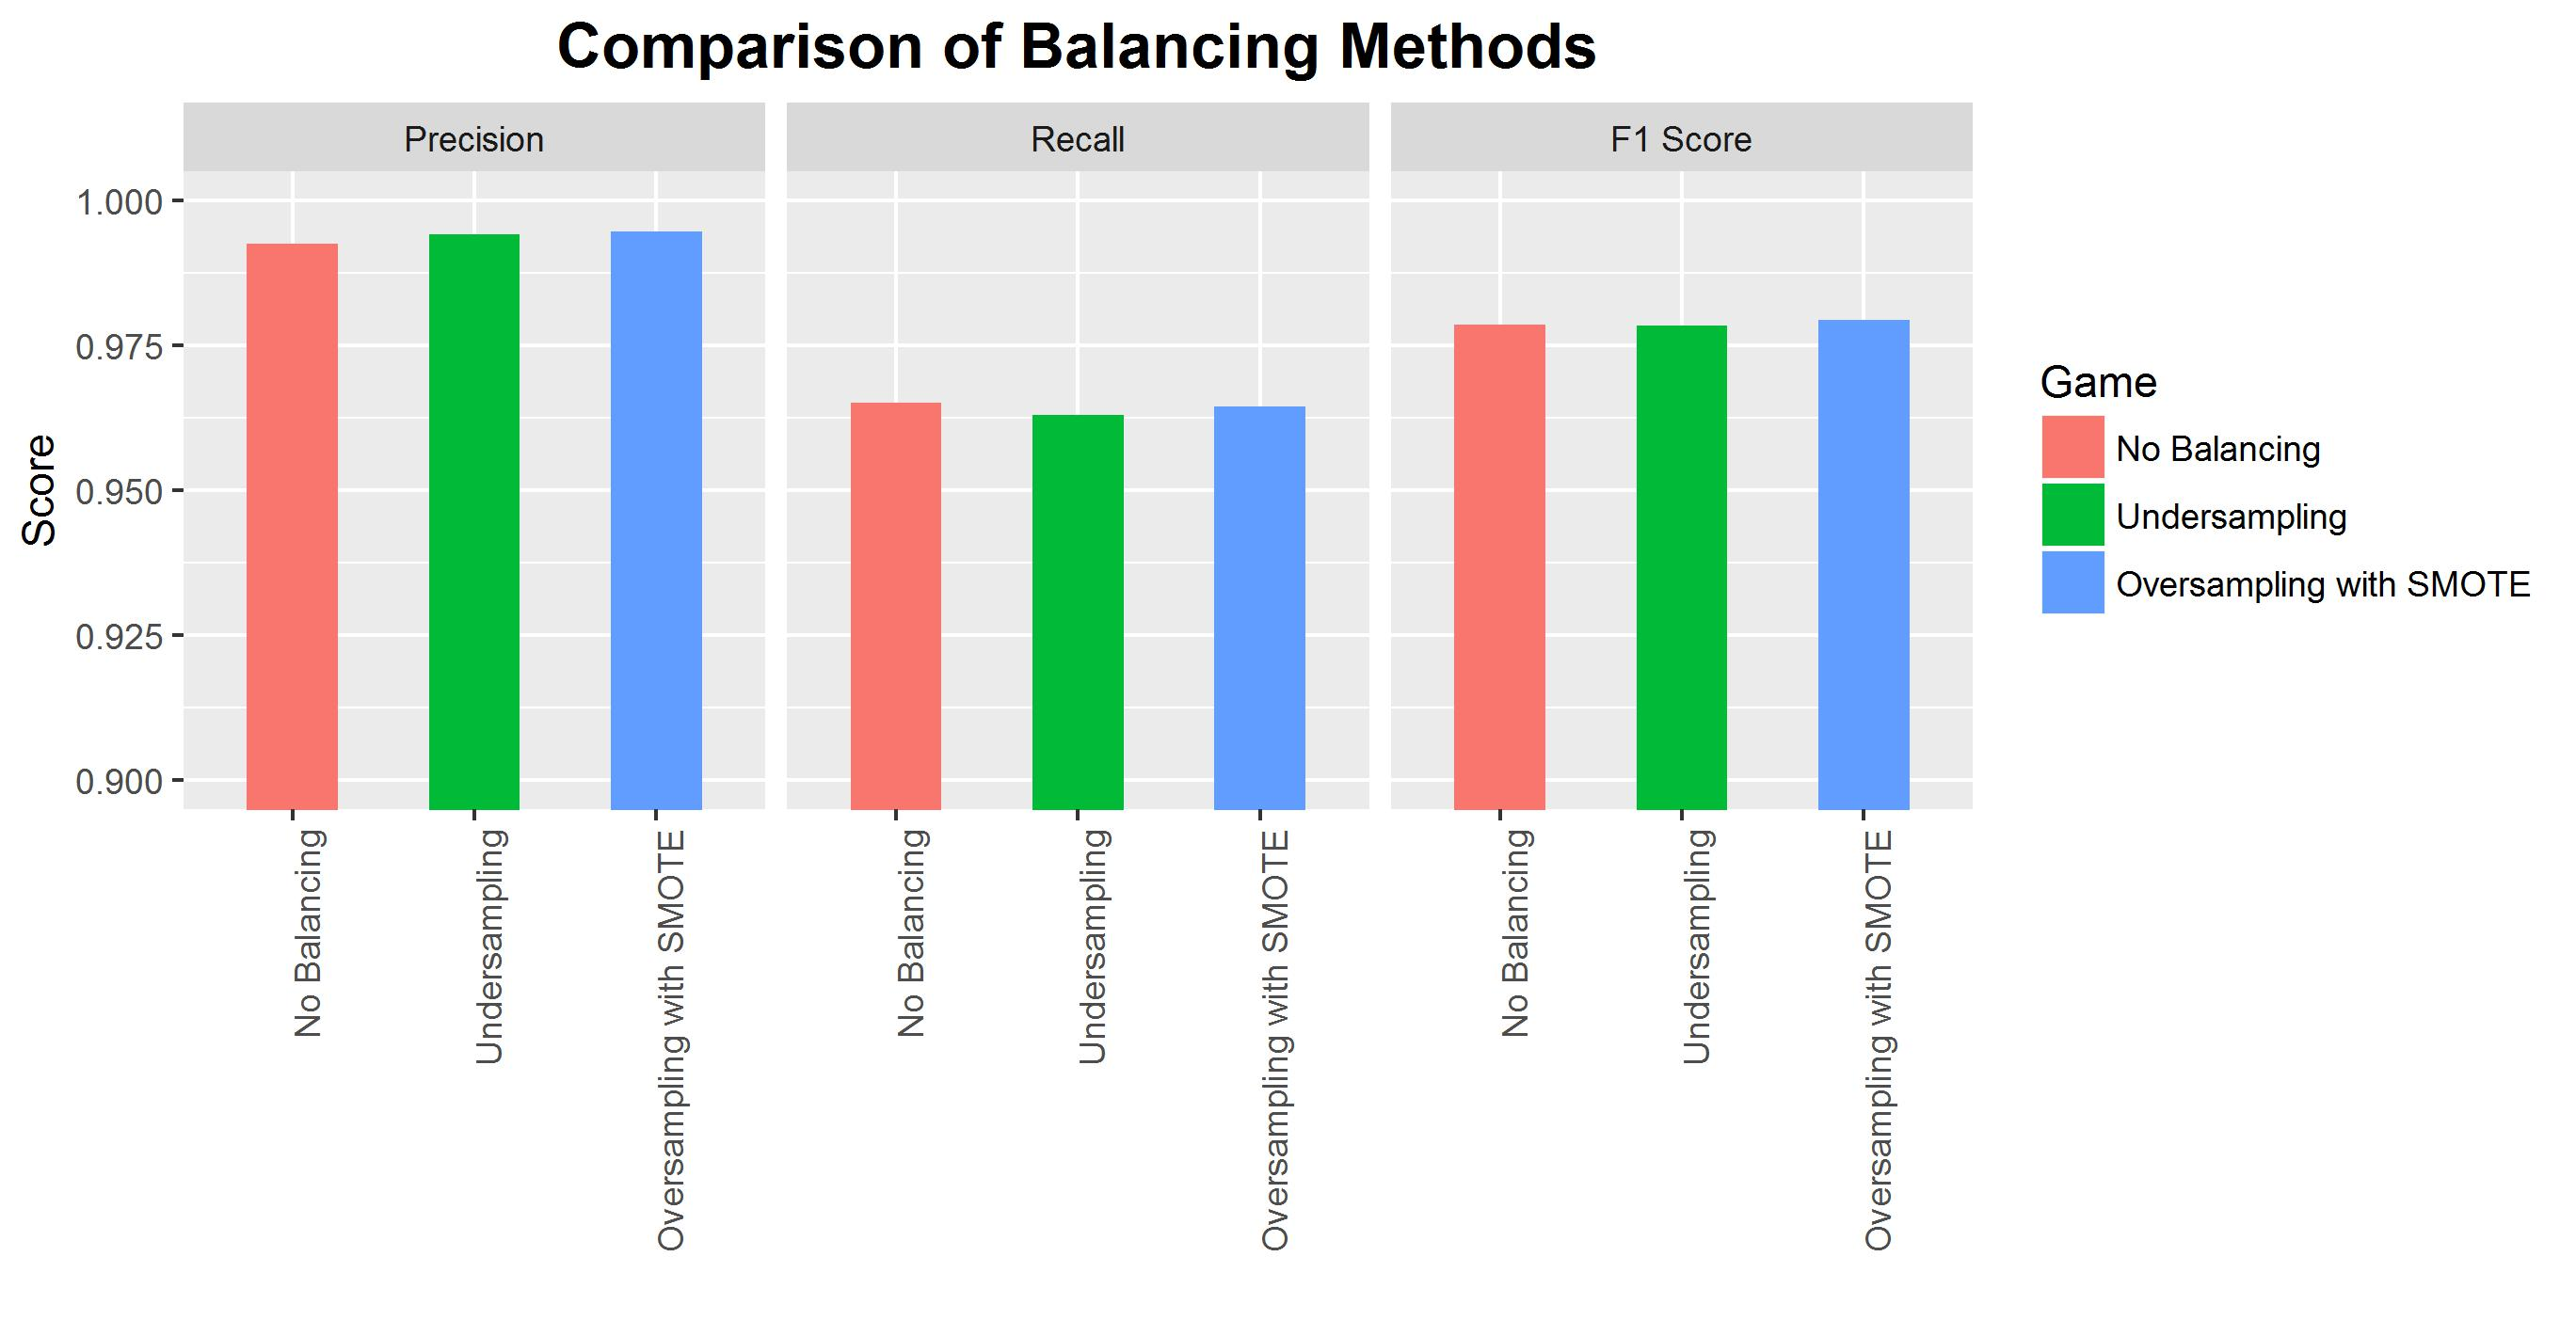
\includegraphics[width=\textwidth]{comparisonofbalancingmethods.png}
\caption{Effect of Sample Balancing on Prediction Ability                 }
\end{figure}
Interestingly, we note that overall, undersampling, oversampling and no sampling at all had very small effects on precision, recall and the final F1 score. Specifically, all three metrics were within a range of 0.003 for oversampling, undersampling and no sampling. This could be due to clear boundary separation within positive and negative class examples as well as good representative datapoints within the positive training example class. This prevents the imbalanced data from having too much of an effect on variant prediction and classification. Still, we note that oversampling techniques resulted in a marginally higher F1 score (0.001 higher than undersampling and no sampling), and since ensuring that datasets are balanced is a recommended protocol to prevent further bias downstream, we used SMOTE oversampling to produce extra positive training class examples for all analysis pipelines.
\subsection{Benchmarking of Optimised Network with Mason Dataset}
From optimisation steps, we finalised the network architecture as seen in Figure 9, but with 8 layers before the merge layer. We chose the learning rate to be $10^{-5}$, and the optimiser used was Adam. With this network, we benchmarked the neural network against the single variant callers, as well as concordance callers, which are an integration of the outputs of the 5 variant callers. Specifically, the n-concordance variant caller is defined as the set of calls that any n callers agree upon - so 1-concordance includes all the calls made by all callers and 4-concordance includes all the calls made by any 4 callers.
\begin{figure}[H]
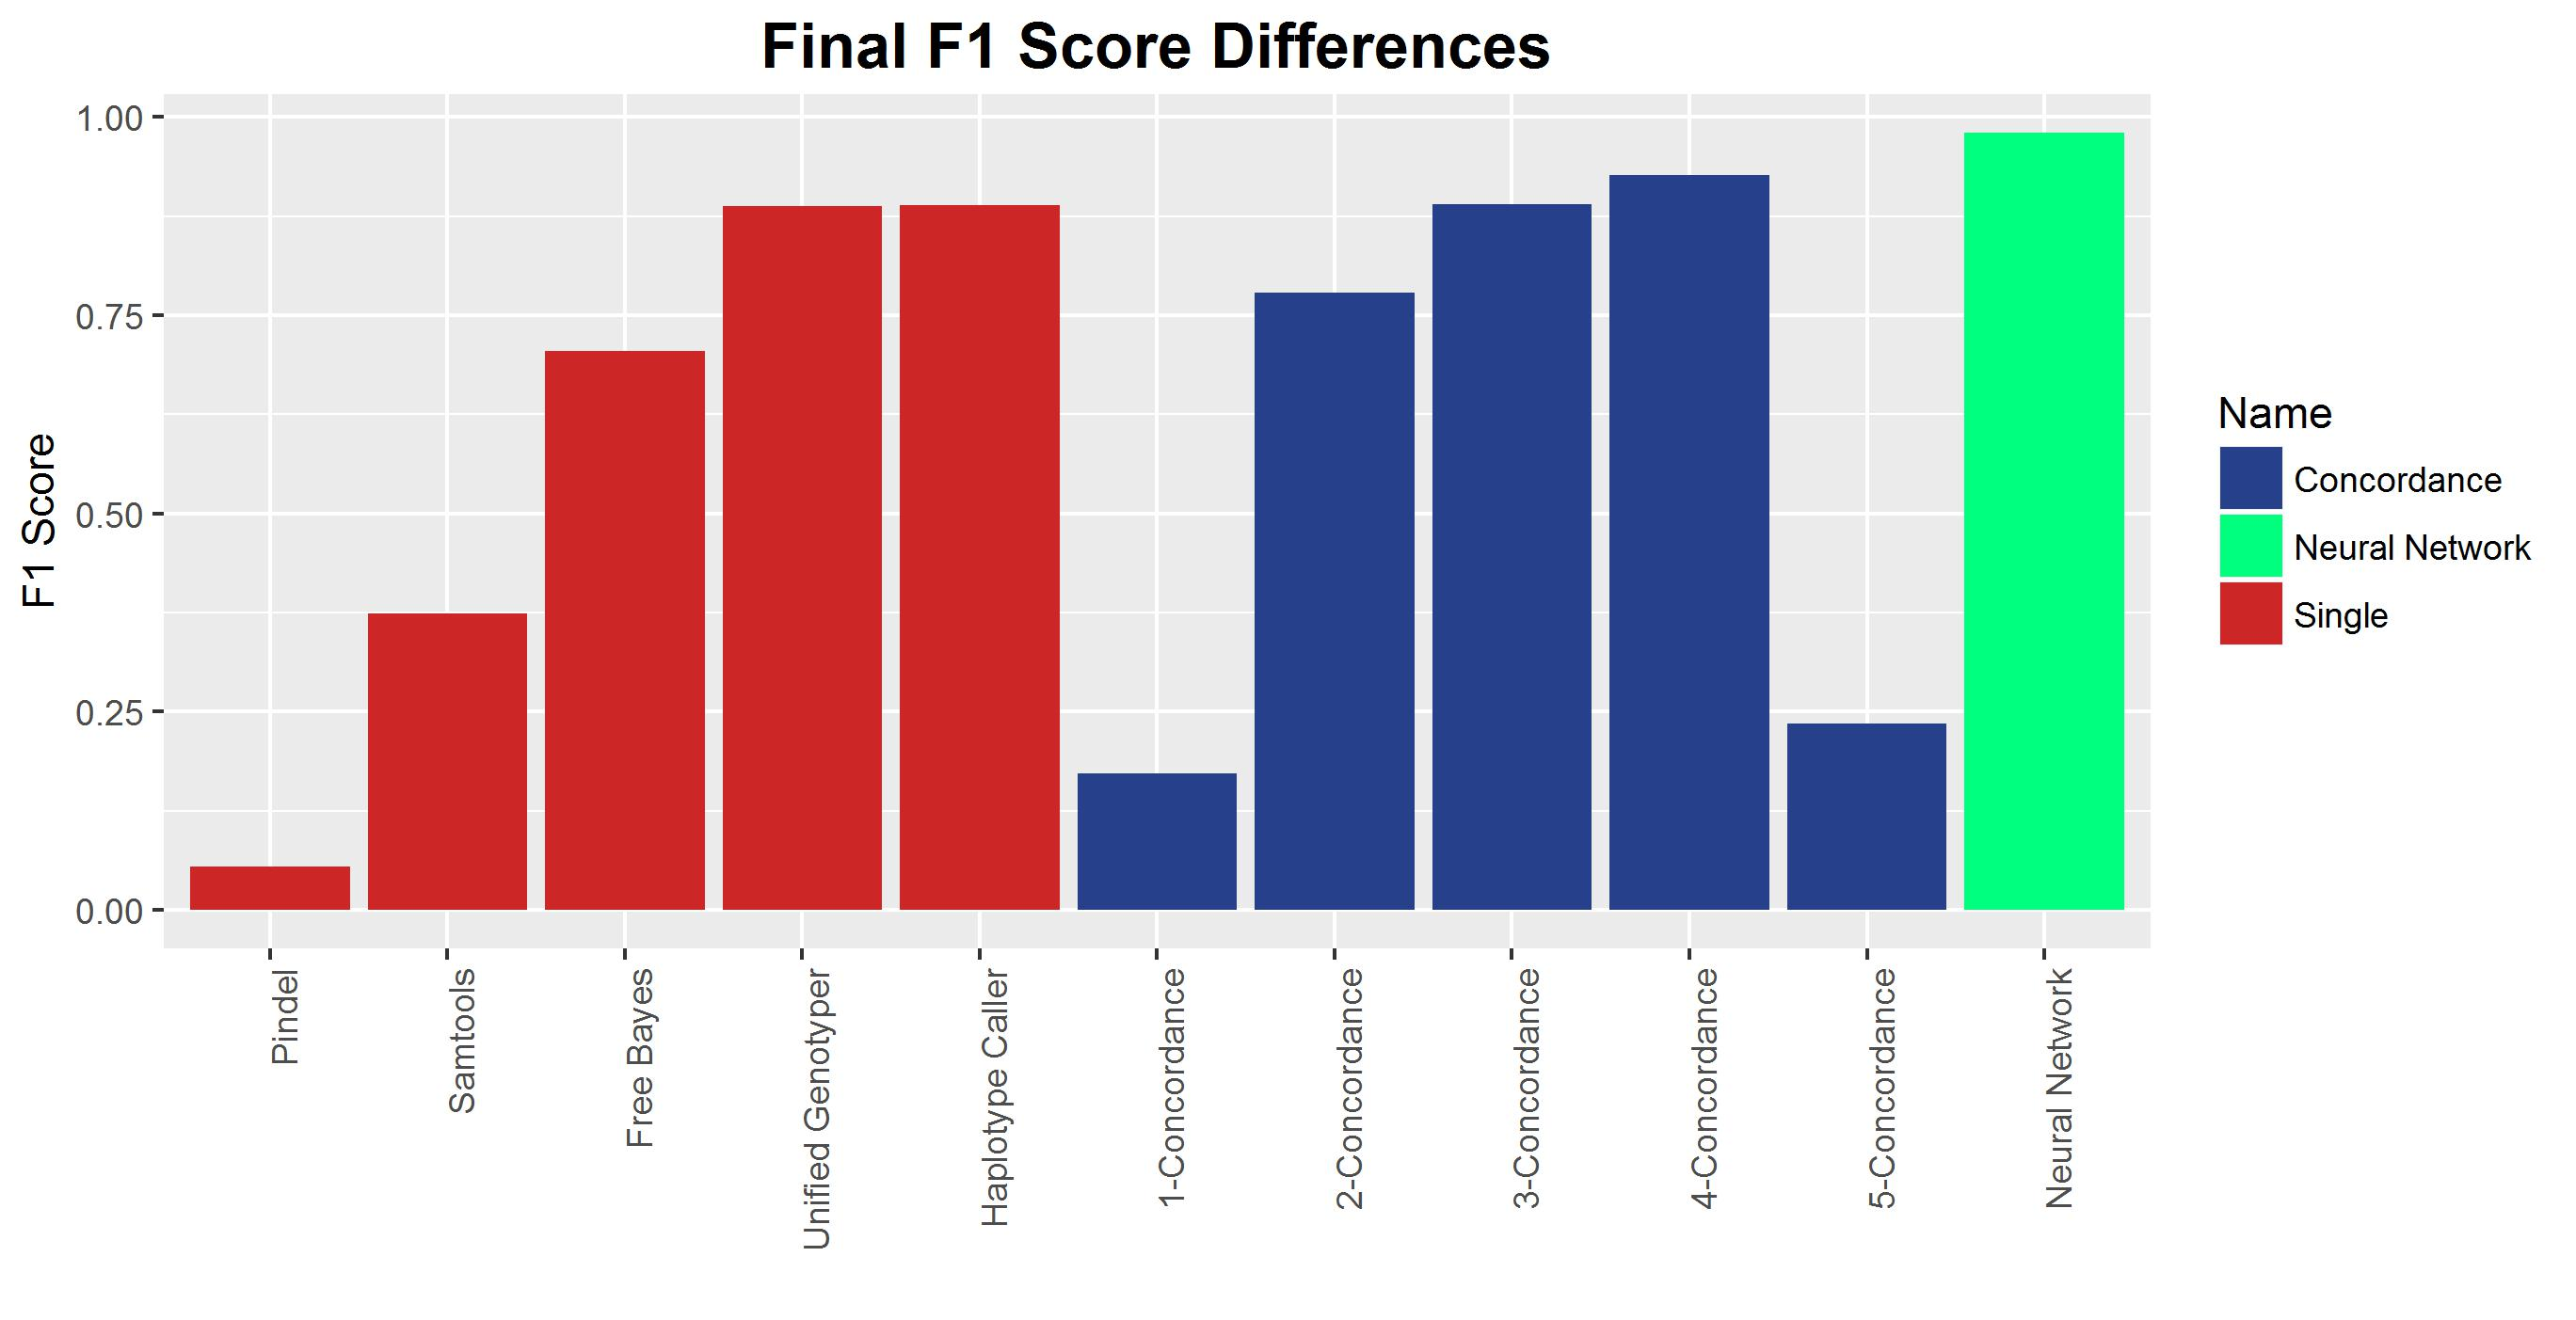
\includegraphics[width=\textwidth]{final_f1scores_results_all.jpg}
\caption{Overall Comparison of Variant Callers}
\centering
\end{figure}
In terms of overall F1 score, we see that the neural network was able to outperform single and concordance-based callers. This provides strong evidence that the neural network is able to learn from the input features whether the variant call is real or not, validating its usage in variant calling. The final F1 score obtained by the best single variant caller was Haplotype caller at 0.888, the best concordance caller had an F1 score of 0.927 while the neural network achieved an F1 score of 0.980. To study whether the increase in F1 score is due to improvements in precision or recall, we studied the exact precision, recall and F1 scores of the top 2 variant callers as well as the best single variant caller versus the neural network. We find that the neural network is more precise than both, but the recall is rather similar. 
\begin{figure}[H]
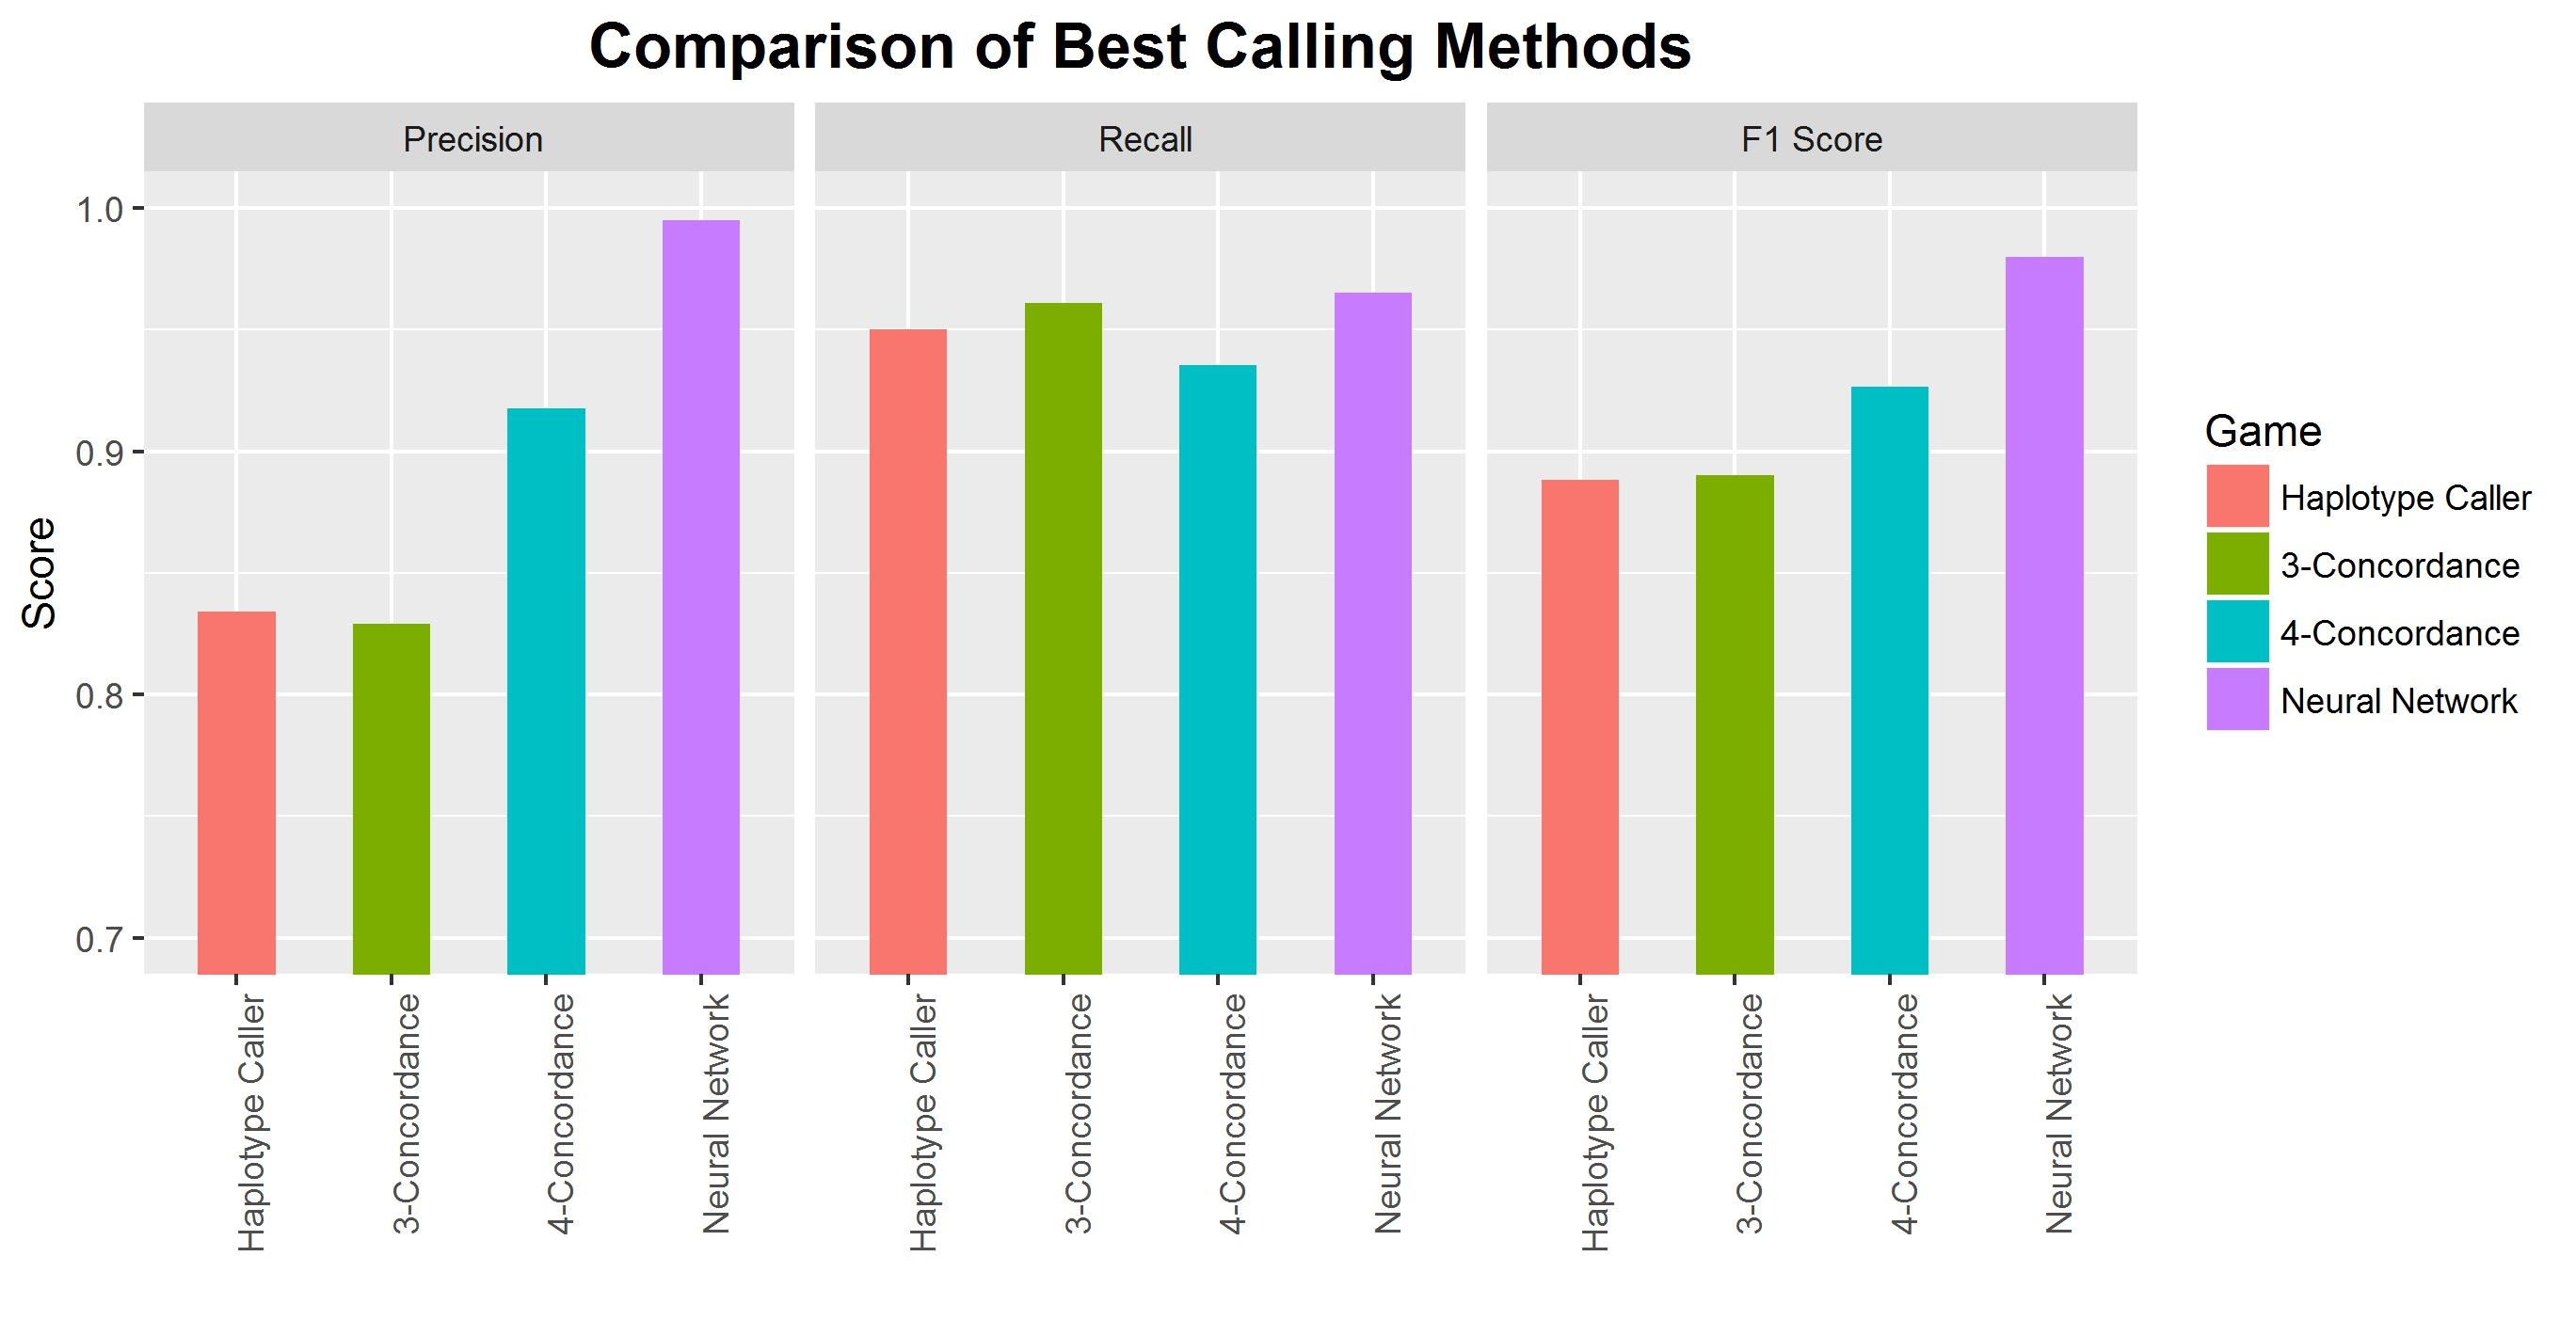
\includegraphics[width=\textwidth]{masonheadsupcomparison.jpg}
\caption{Comparison of Best Variant Callers in terms of Precision, Recall and F1 Score}
\centering
\end{figure}
We find that the neural network is more precise than all four callers, with the neural network had a high precision of 0.995 compared to only 0.917 for 4 concordance. This is a 20 fold decrease in the number of false positives or about 23,000 more false positive calls in the 4 concordance network compared to the neural network. Interestingly, the recall of all the callers was high in the range of 0.90 to 0.95, indicating that while all were able to pick out most of the truth class variables, the main errors came from a high number of false positives that were also called as true mutations. Ultimately, the neural network had an F1 score that was 0.1 above the best single caller and 0.06 above the best concordance caller. Thus, this provides strong evidence that the neural network is able to sieve out false positives within the dataset and stably predict whether a mutation is true.
\subsection{Benchmarking of Optimised Network with NA Dataset}
After verification of the neural network architecture, optimised parameters and ability to learn with a simulated dataset, we sought to analyse a real dataset to set the validity of the neural network in validating variants. We studied the NA12878 Genome In a Bottle dataset (Zook et al., 2014), which has been used in other variant calling validation pipelines(Talwalkar et al., 2014; Linderman et al., 2014) and contains a set of high-confidence variant calls which we can use as ground truth for training and validation. This set of high-confidence variant calls is obtained from multiple iterations of orthogonal sequencing methods (using Solid, Illumina platforms, Roche 454 sequencing and Ion Torrent technologies). The usage of multiple platforms enables an intersection of variants that can be considered as the ground truth. We then sought to see if our neural network can predict the ground truth better than single or concordance based variant callers. \\\\We applied the same methodology to the sequences as with the simulated data and then used our neural network to predict the true variants. Validation was done with 47971 high-confidence variant calls.
\begin{figure}[H]
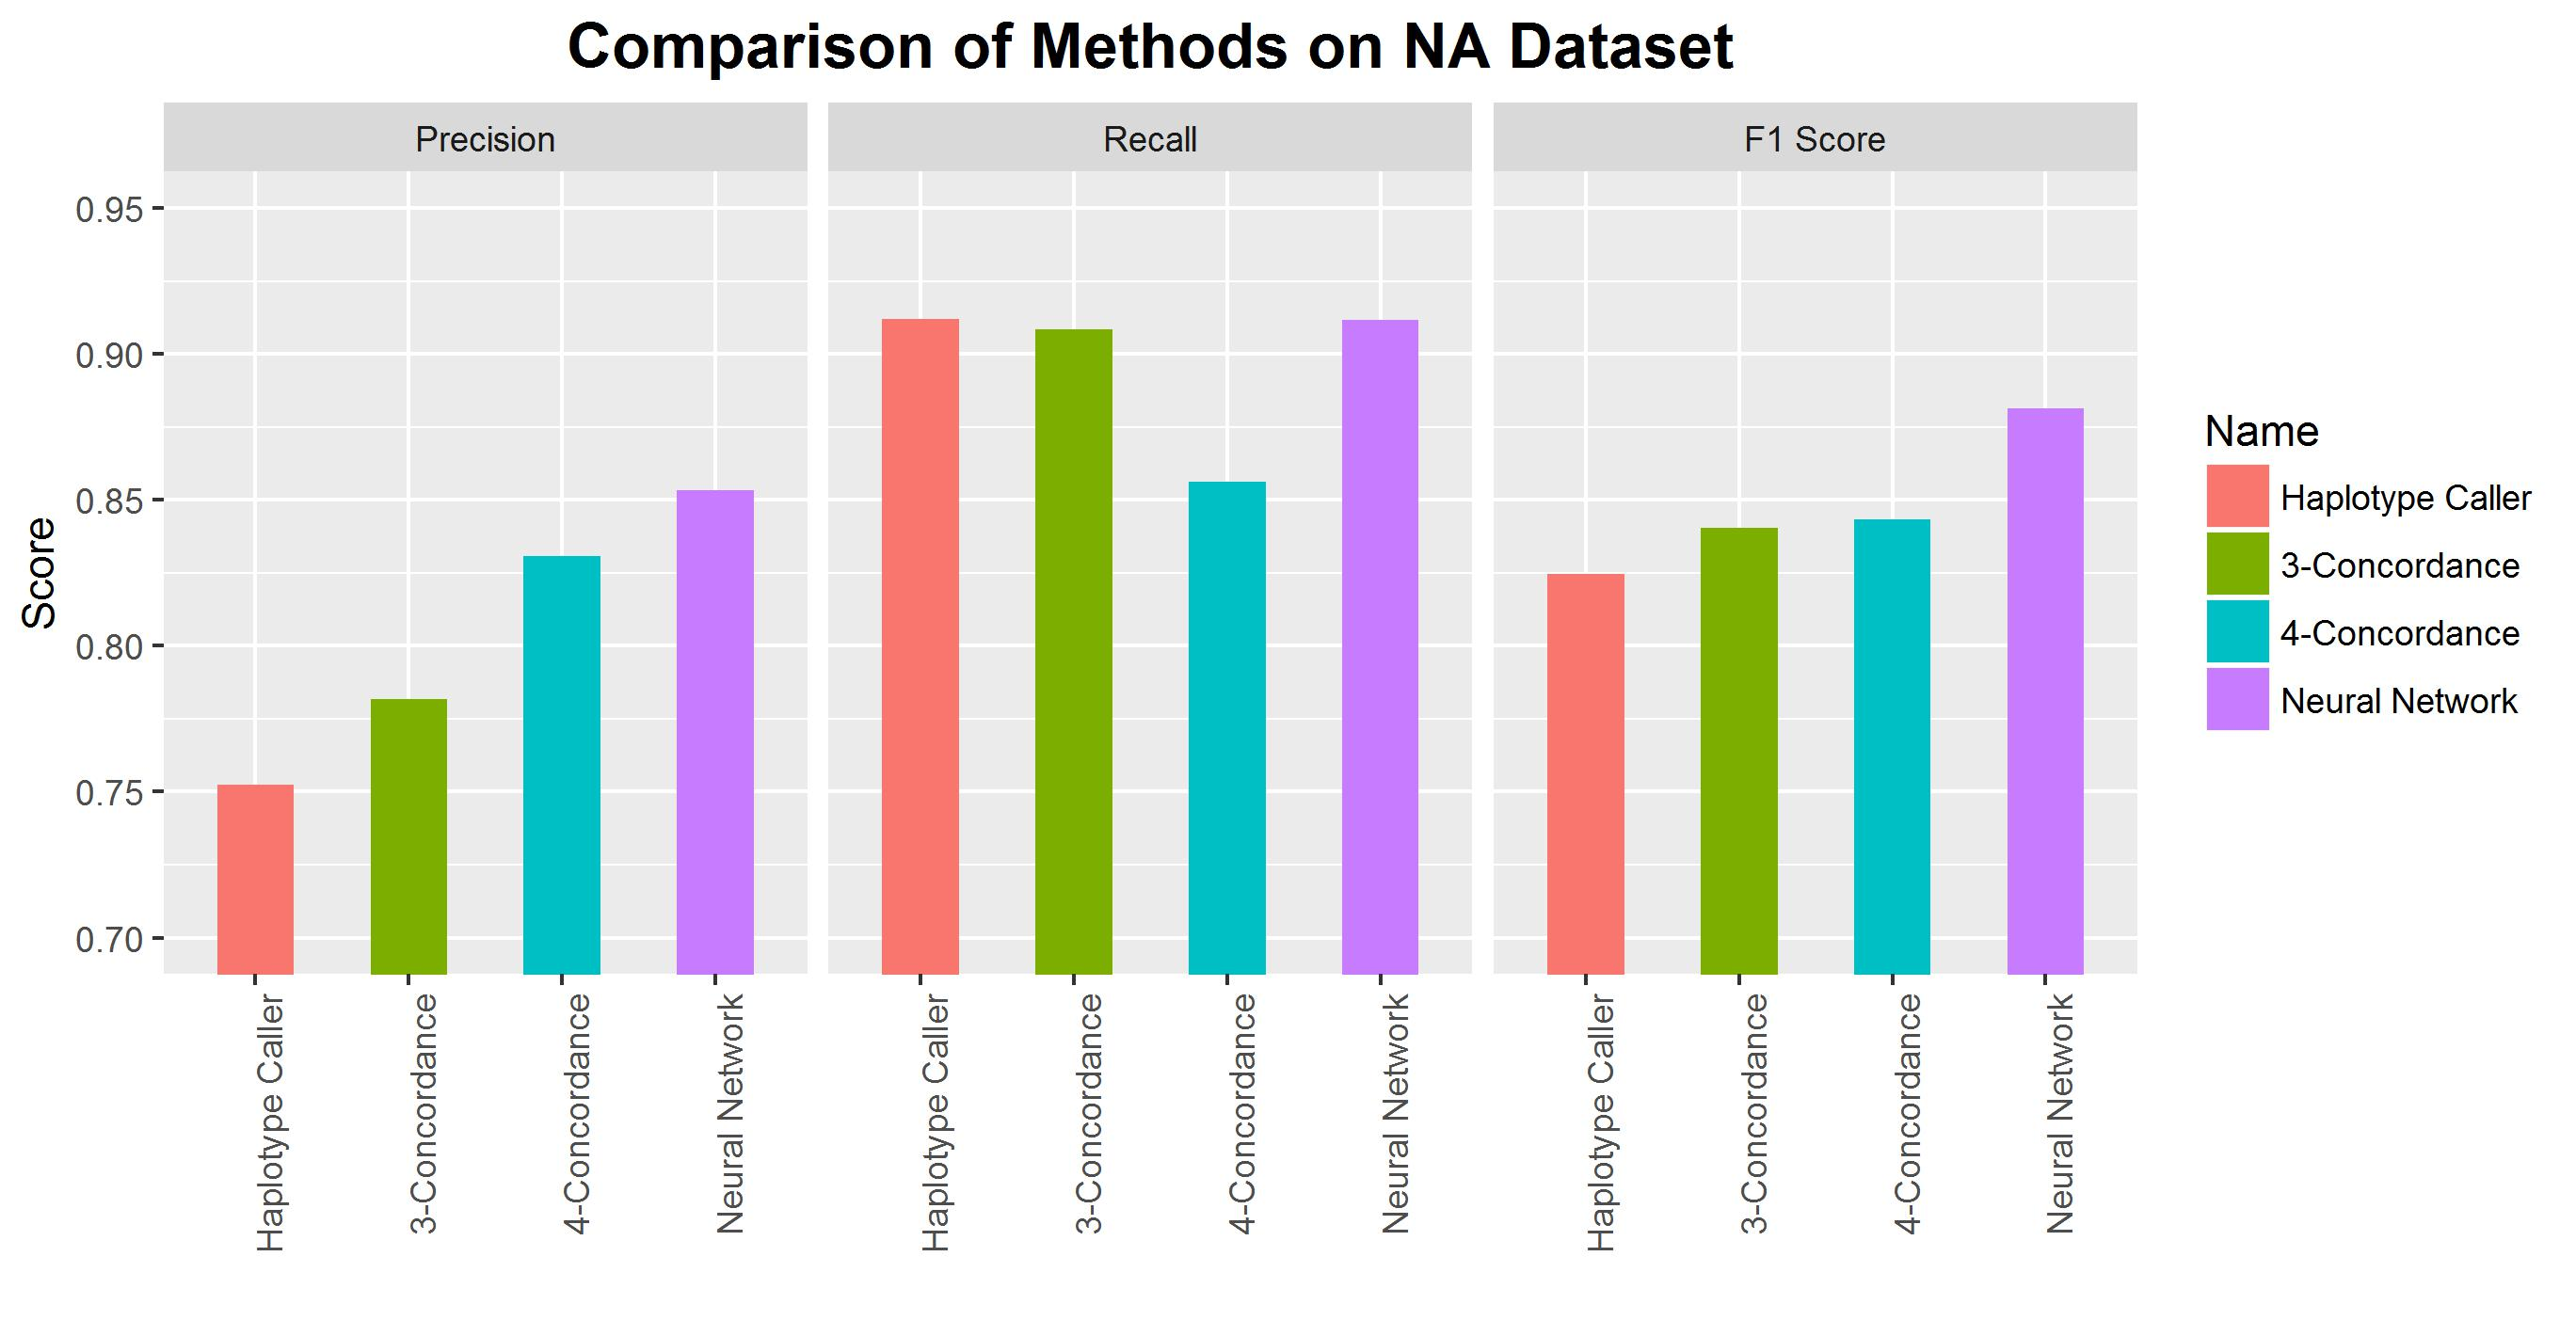
\includegraphics[width=\textwidth]{naheadsupcomparison.jpg}
\caption{Comparison of Variant Callers}
\centering
\end{figure}
As can be seen from the figure, the neural network was able to predict with the highest precision (0.859) when compared the best single caller, haplotype caller (0.752) and the 2 best concordance callers, 3-concordance (0.782) and 4-concordance (0.830). In terms of recall, the neural network had a higher recall (0.911) compared to the 4 concordance caller (0.856). Thus, we see that in the NA dataset, the neural network compared with the 4 concordance network is able to call 2650 true variants that were missed by 4 concordance and still had 1228 less false positives. This means the neural network was more aggressive in making calls, yet more of the calls were correct. Compared to the three concordance caller, the neural network had 4253 less false positives. Ultimately when we looked at the F1 score, the neural network was able to outperform concordance variant callers by at least 0.04 and single callers by 0.06. This validates our neural network pipeline in a real genomic dataset and indicates that network is able to learn from the input features.
\newpage
\subsection{Analysis of Gene Importance using Bayesian Ranking systems}
After validation of high confidence calls, we sought to enable a clear and understandable ranking of genes. We first build a Bayesian network analysis using known functional annotations from ANNOVAR. These were subsequently used to compute the Bayesian probability ranking, which is shown in Figure 17 below.


\begin{figure}[H]
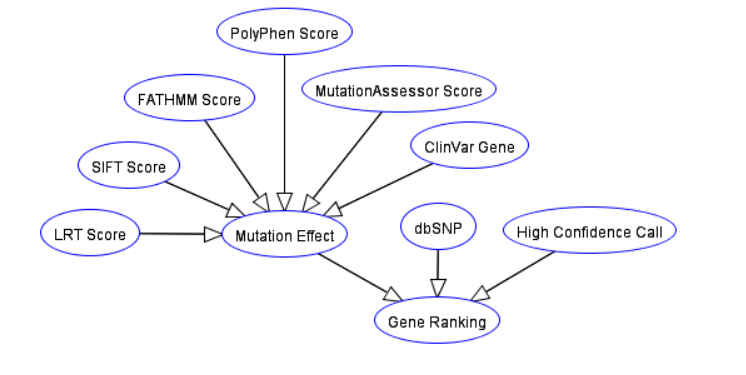
\includegraphics[width=\textwidth]{bayesiannetwork.png}
\caption{Final Bayesian Network used in Analysis}
\centering
\end{figure}

This network structure was chosen as we wanted to use three different sets of information to update the probability of the gene being important. Firstly, the confidence of the call should matter in how important it is - the more likely a gene is real, the more important it should be. Secondly, the rank should also be determined by how common the variation is, based on studying known SNP polymorphism rates. If it is a common SNP, then the ranking should be downgraded as it is less likely to be a driver mutation (Schork et al., 2009). Finally, we sought to predict the overall effect of mutations via an ensemble of mutation effect predictors. These predictors use different methods to predict the average effect of that mutation - based on statistical methods like position-specific substitution matrixes and Hidden Markov Models to study the effect of a mutation on protein structure and function. We also used the ClinVar database, a curated repository of known Human variants and their resulting phenotypes (Landrum et al., 2014). These scores were then aggregated to update the probability of the mutation effect. To obtain these functional annotations, the informatics tool ANNOVAR (Wang, Li, \& Hakonarson, 2010) was used. Table 3 shows the functional annotations obtained from ANNOVAR and how they were computed.

\begin{table}[H]
\caption{Table of Functional Annotations obtained from ANNOVAR}
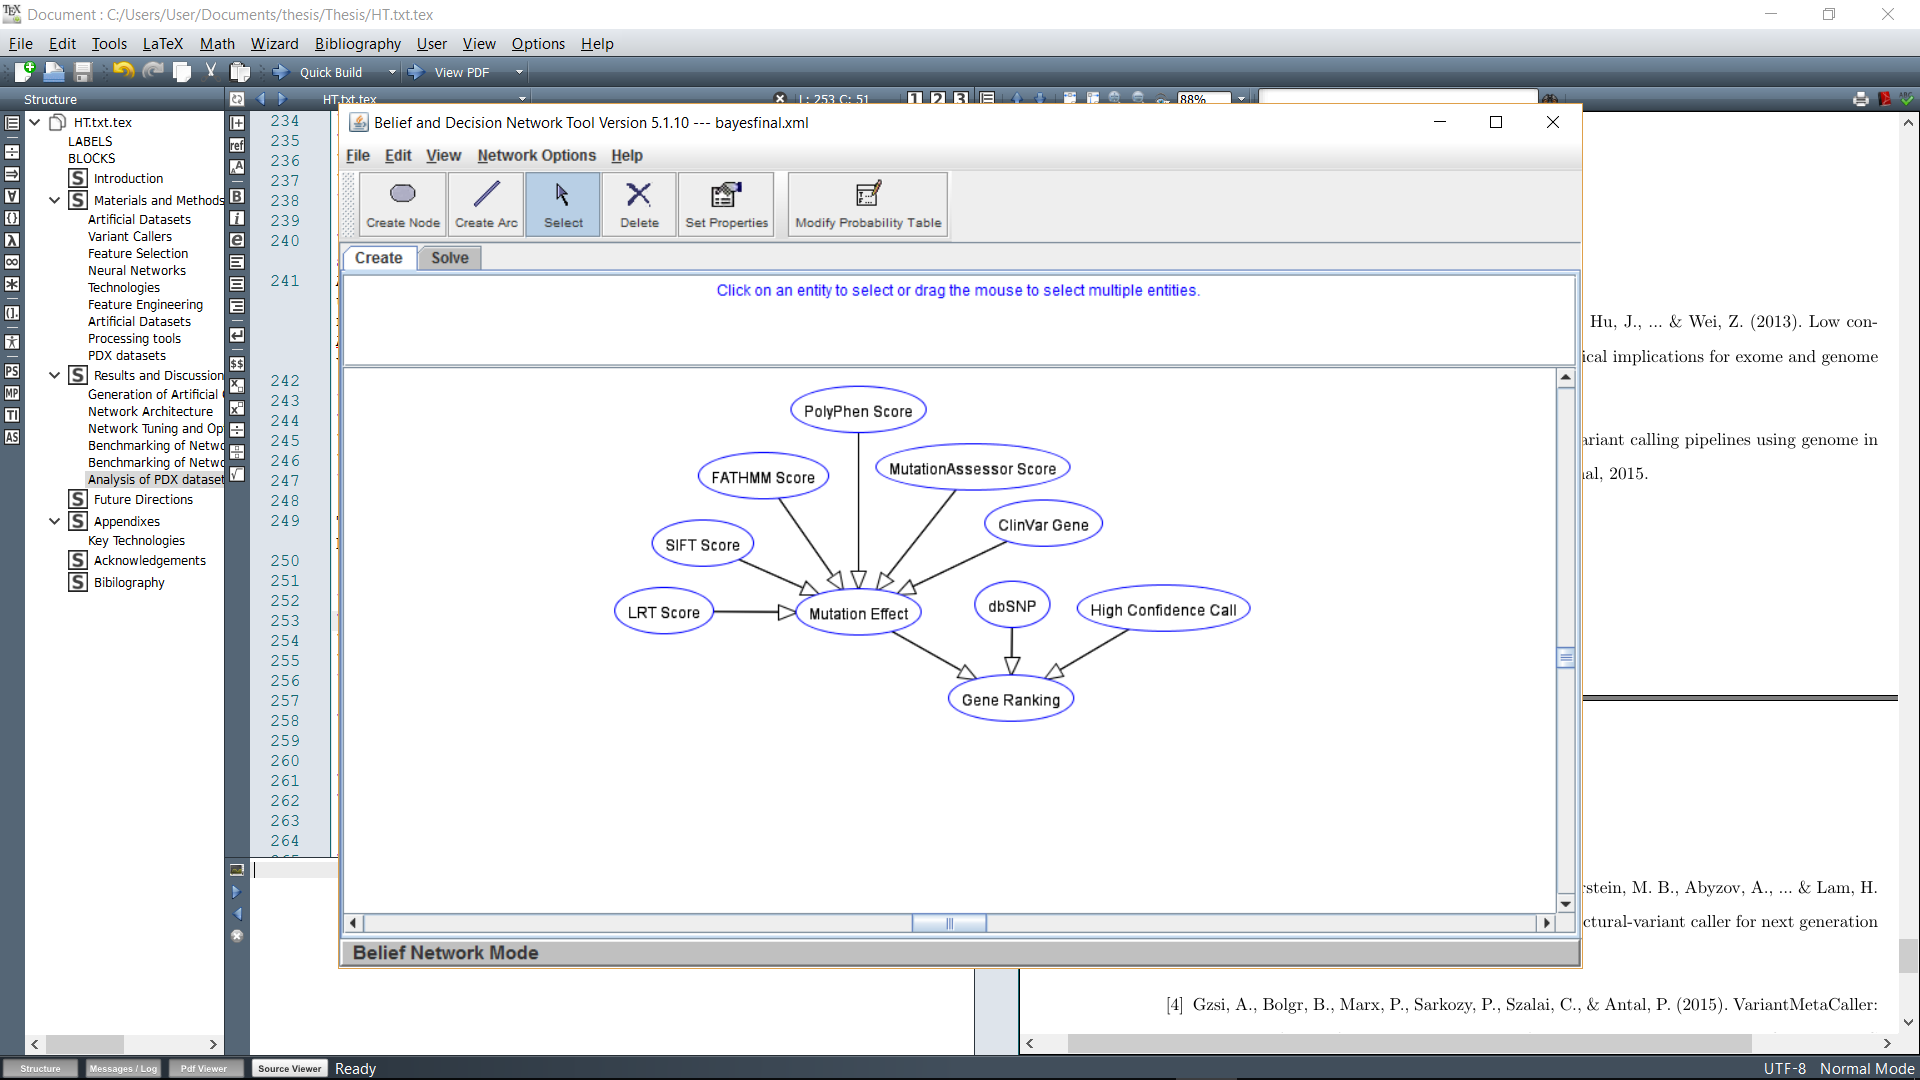
\includegraphics[width=\textwidth]{annovarfeatures.png}
\centering
\end{table}


Based on scores provided, we report the update the conditional probabilities using the probabilities chain rule - for the first level, this is given as \\
\begin{equation}
\begin{split}
P(Impt | (Del  \ \cap \ Uncom  \cap High\ Conc)) =  \ \ P(&Impt \cap Del  \ \cap \ Uncom \cap High \ Conc ) \\ \ * \ & P(Del  \cap Uncom  \cap High \ Conc )
\end{split}
\end{equation}
\tiny
\indent
P(Impt) refers to the probability of the gene being important,\\
\indent P(Del) refers to the probability of the gene being deleterious,\\ 
\indent P(Uncom) refers to the probability of the gene being uncommon and\\  \indent P(High Conc) refers to the probability of the gene being a high confidence call.\\ \indent Further calculations can be found and derivations can be found in Appendix A\\

\normalsize
\noindent
To compute the final probabilities, the software pomegranate was used. This simplifies the node drawing and probabilistic updates of the final ranking scores.
\subsection{Validation of Bayesian Network Ranking on PDX dataset}
To study the effectiveness of our Bayesian network ranking system, we sequenced and analysed a patient-derived xenograft (PDX) tumour genome. This tumour genome was grafted onto the immunocompromised mouse from a patient with a known cancer subtype - Diffuse Large B-Cell Lymphoma (DLBCL). We chose to analyse lymphoma as it is a well-known and studied disease model with a well-defined disease progression (Knudson et al., 2001; Alizadeh et al., 2000). The patient-derived xenograft model also allows \textit{in vivo} studies of the tumour in its environment and serves as a good model for sequencing and analysis (Tentler et al., 2012). After sequencing the PDX genome, we put it through our full analysis pipeline, which involves identifying high-confidence mutations using the neural networks and then ranking these genes using the Bayesian network ranking. Figure 19 shows the top 30 genes by probability. 

\begin{figure}[H]
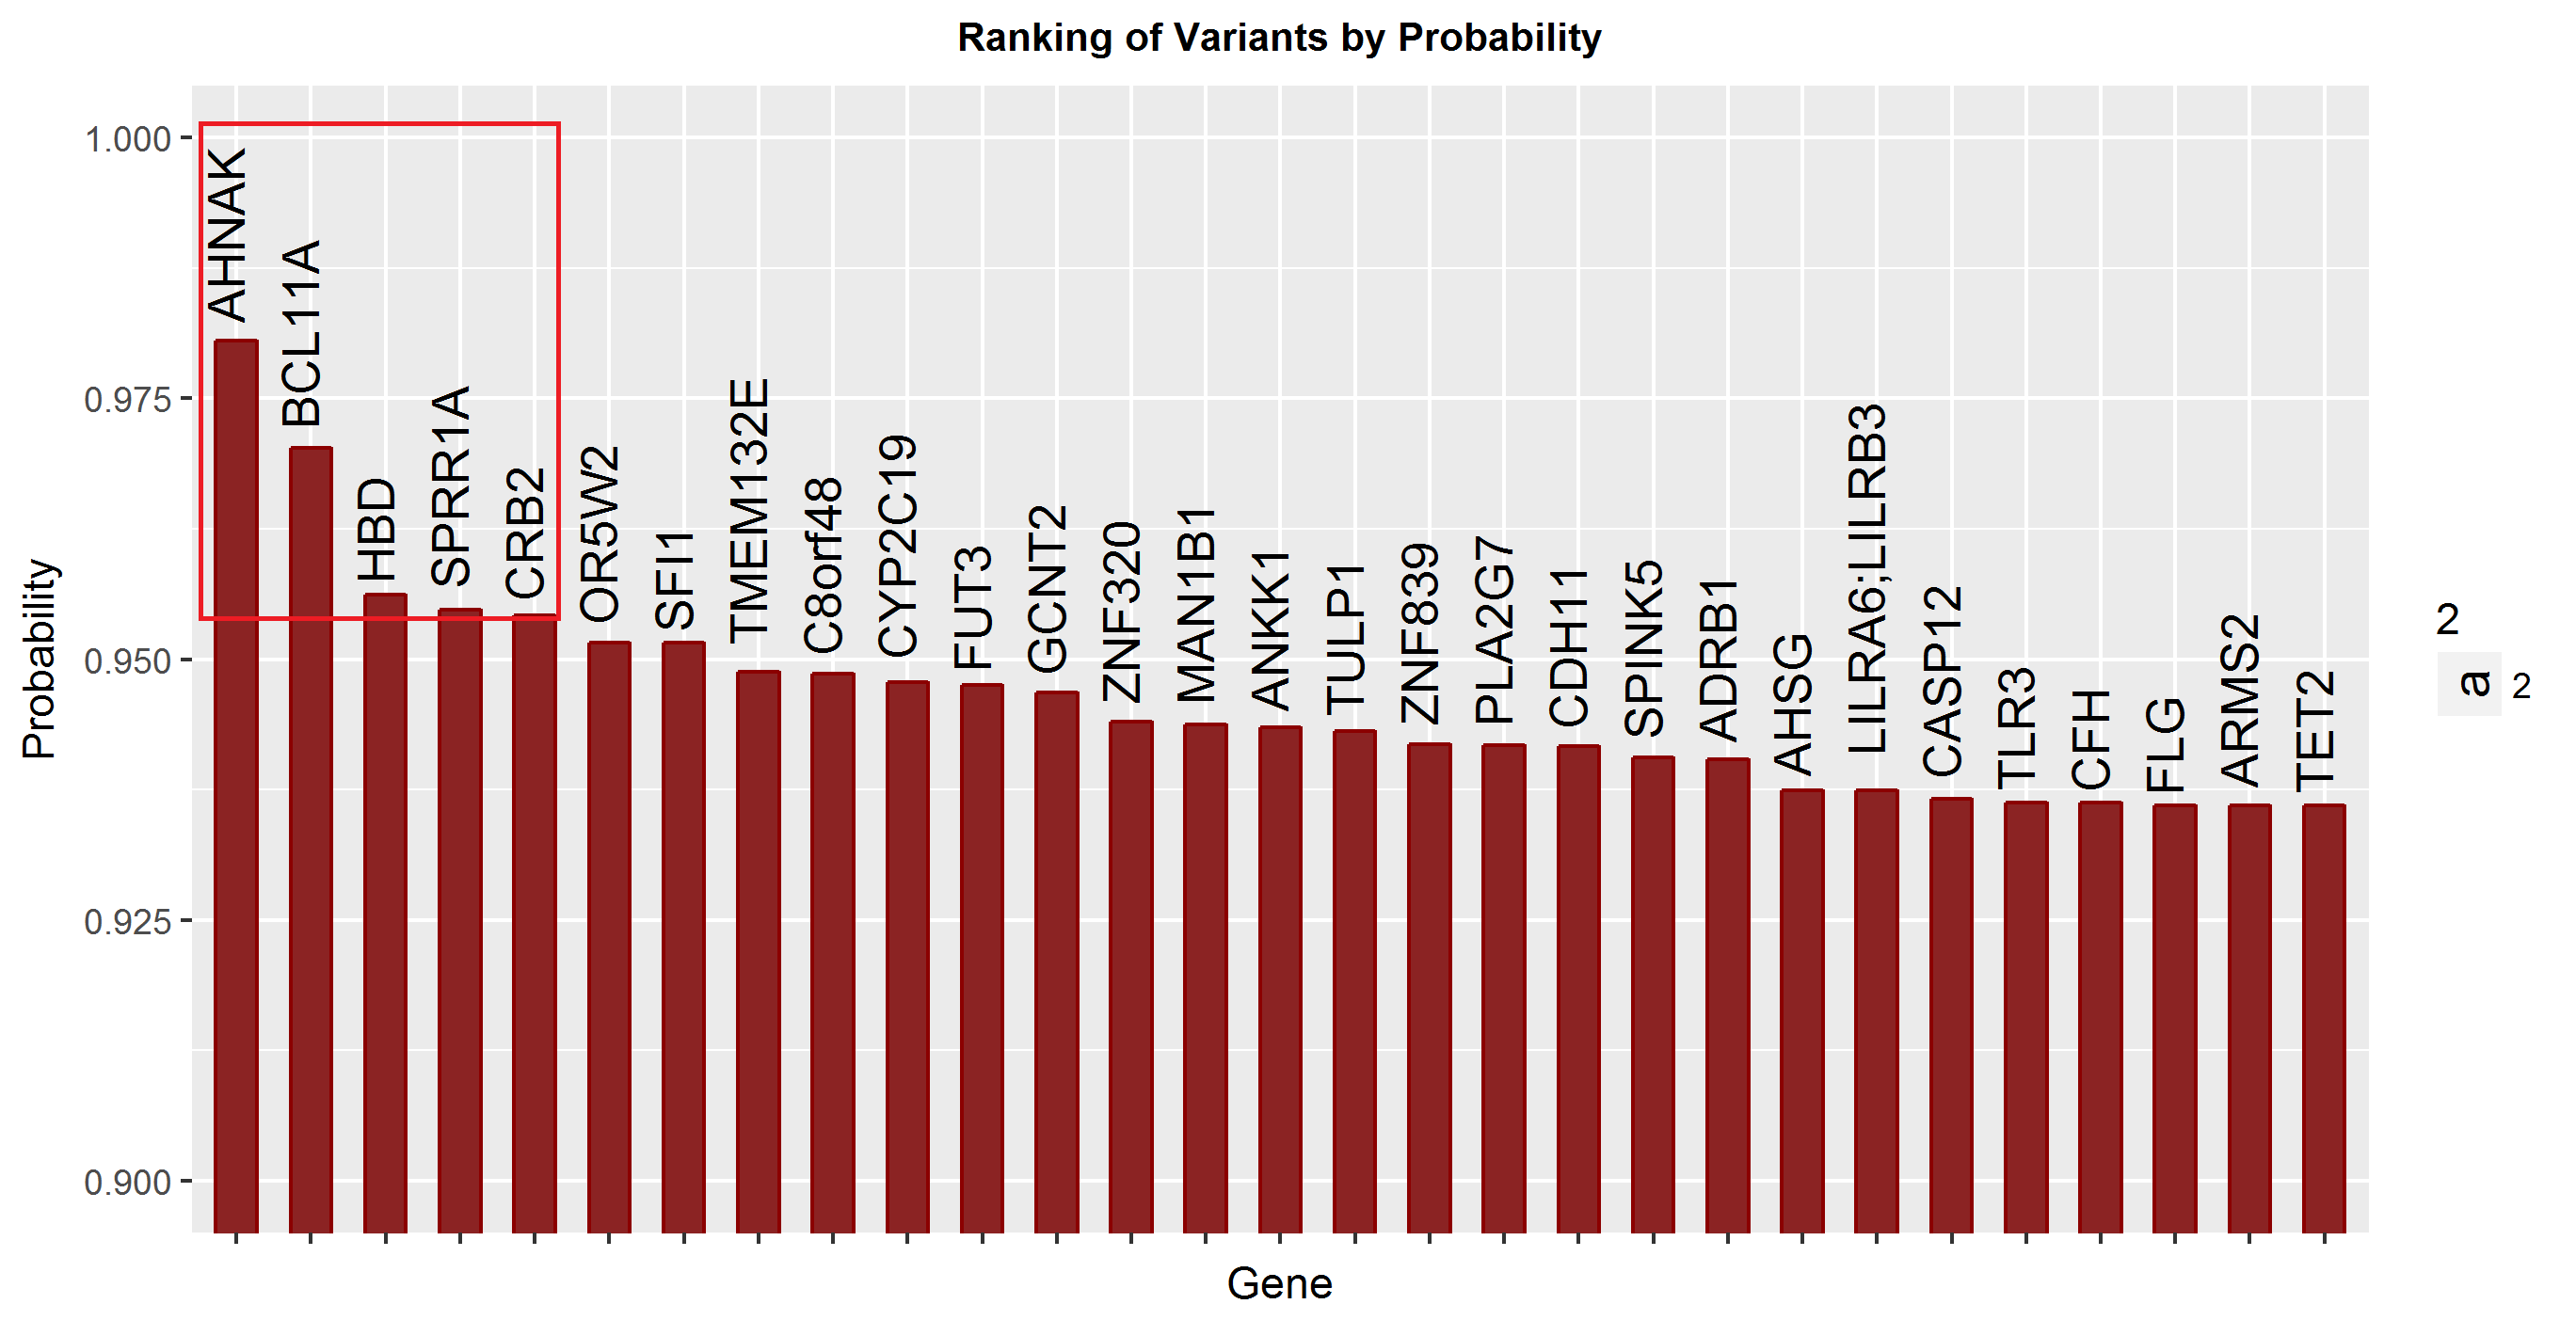
\includegraphics[width=\textwidth]{bayesianranks.png}
\caption{Top 30 genes from Bayesian Ranking Algorithm}
\centering
\end{figure}

Studying the top 5 genes, we found that four of these five genes have been implicated in lymphomas or other cancers. AHNAK is a known tumour suppressor and has been known to be downregulated in lines of Burkitt Lymphoma. BCL11A is a known proto-oncogene in DLBCL and has been found to be overexpressed in 75\% of primary mediastinal B-cell Lymphomas, a subset of DLBCL. SPRR1A, the fourth gene ranked in terms of importance, has been shown to be expressed in DLBCL and its expression has been shown to strongly correlate with 5-year survival rate (Figure 21). Finally, development of B-cell lymphoma has been noted in Crb-2 related syndrome, which is a bi-allelic mutation of CRB2. Interestingly, the last of the high ranked genes was noted to be a subunit of Hemoglobin. While there is no strong evidence for the role of Haemoglobin in DLBCL, it has been shown to be expressed in aggressive glioblastomas lines, indicating a possible previously unknown role in cancer. This gives us high confidence that the Bayesian ranking network is able to pick up important and relevant mutations. Without such a ranking system, we would have to look through over 70 thousand genes, without a way to systematically study their likelihood of being important. 

\begin{figure}[H]
\caption{Table of Top 5 important genes from Bayesian Ranking}
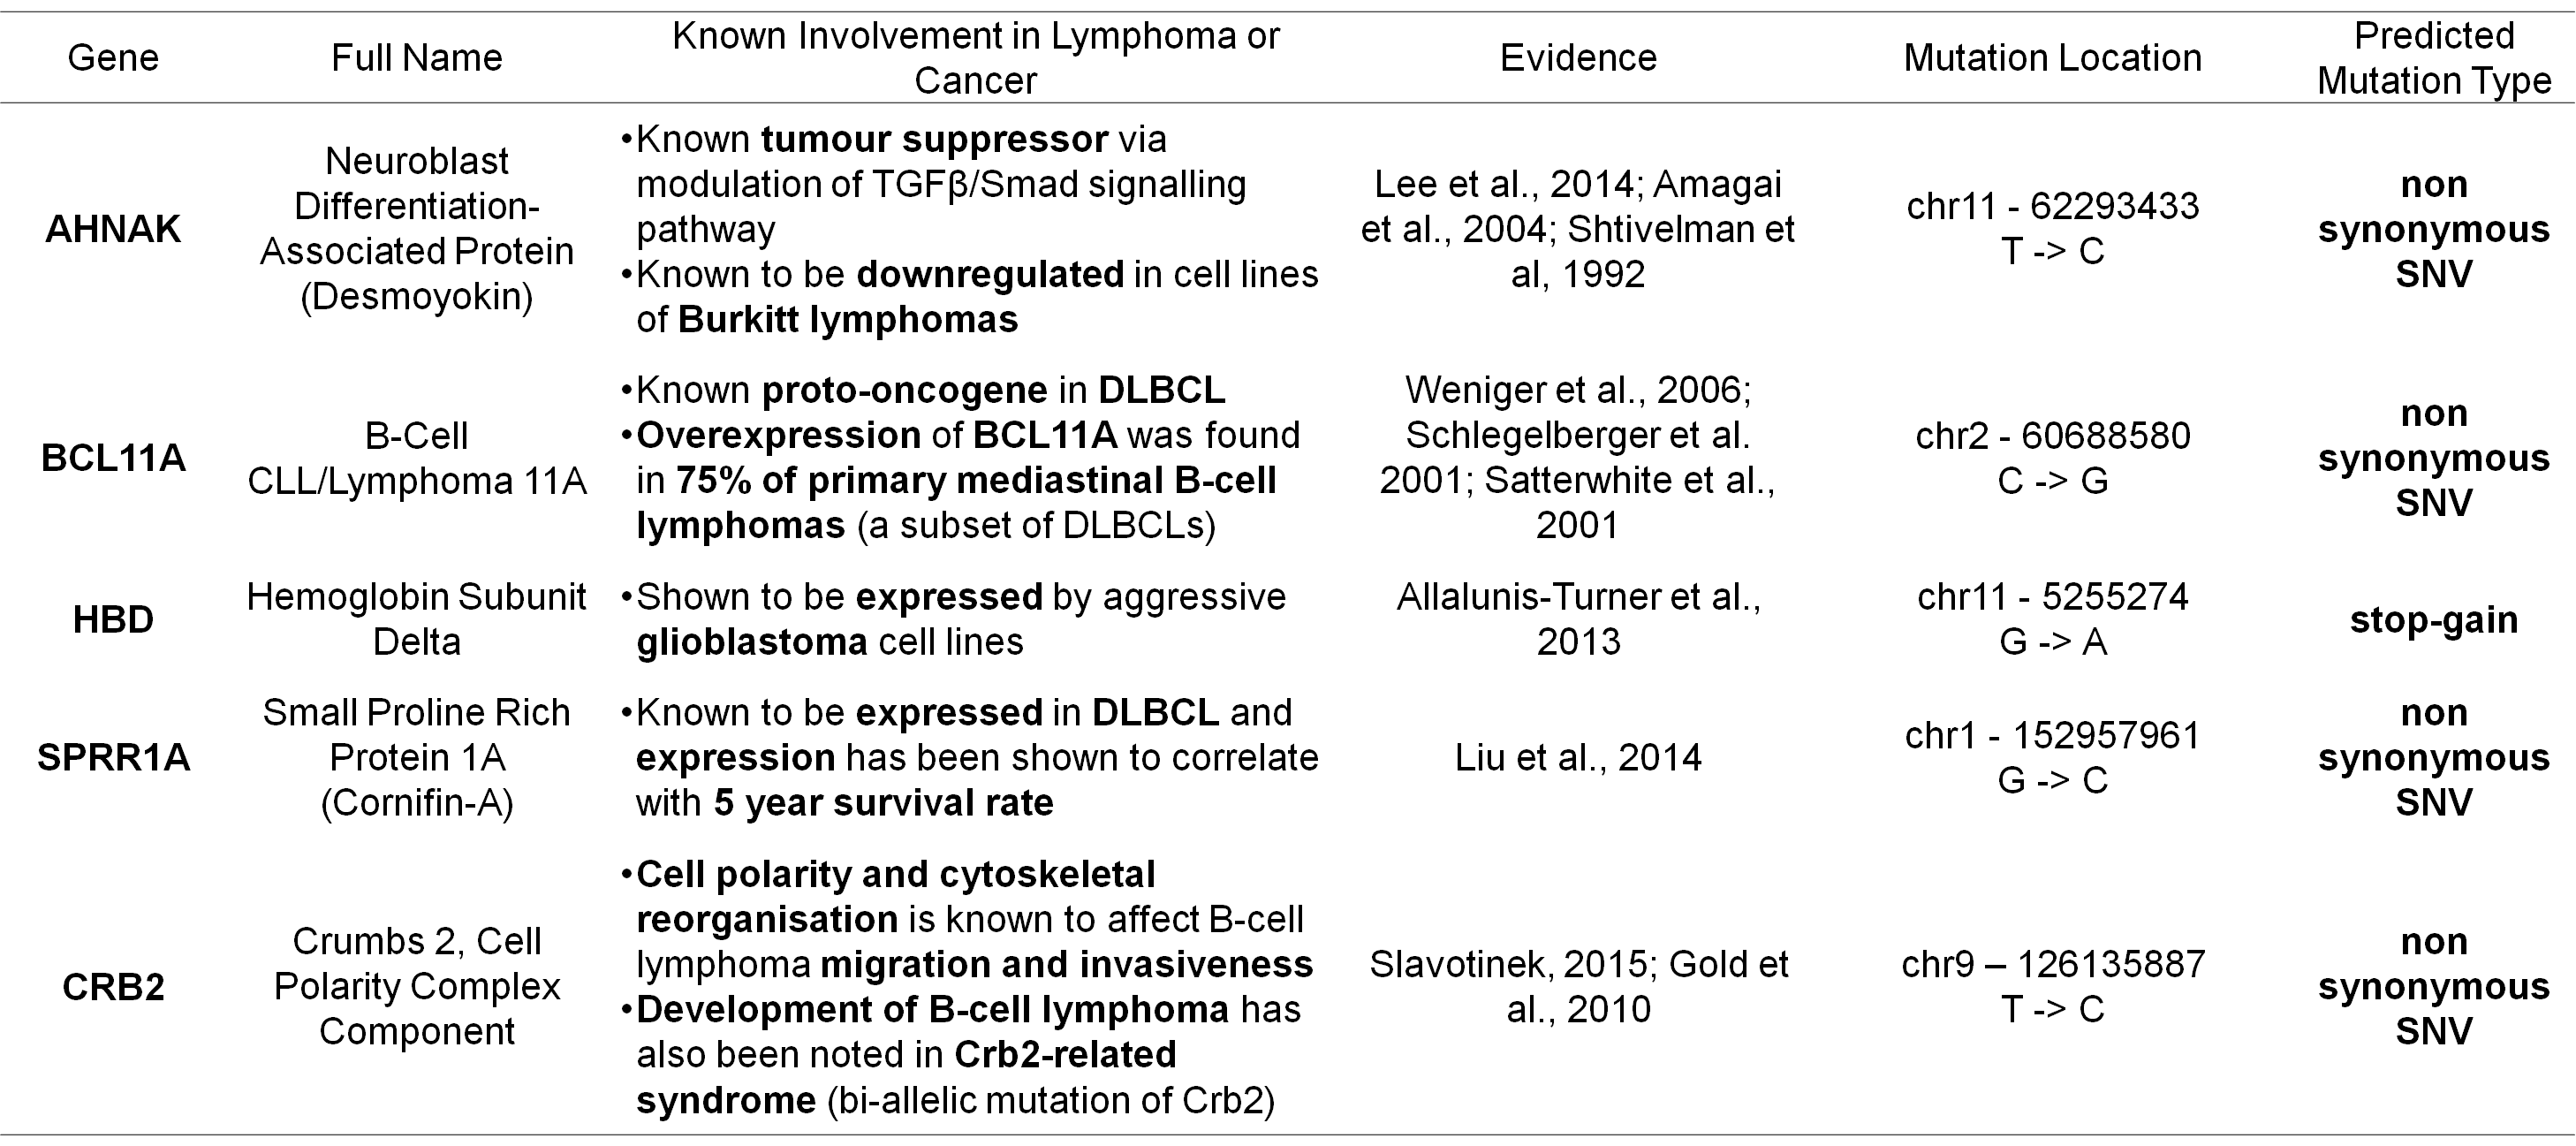
\includegraphics[width=\textwidth]{top5importantgenes.png}
\centering
\end{figure}

\begin{figure}[H]
\centering
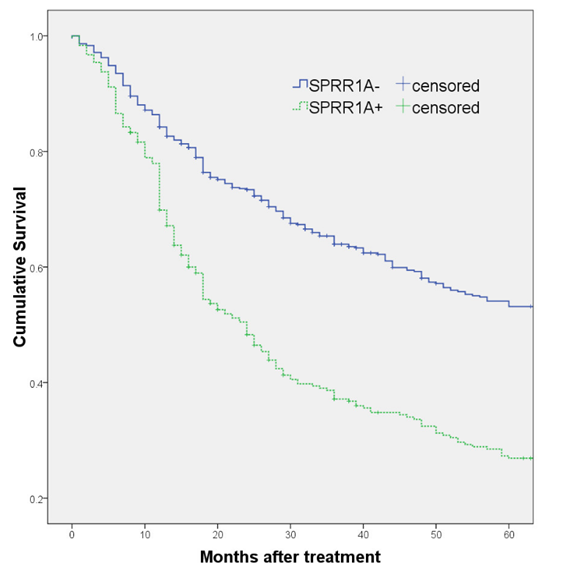
\includegraphics[width=0.5\textwidth]{sprr1adataset.png}
\caption{5 year survival curve of patients with SPRR1A+ and SPRR1A- patients with DLBCL. Source : Zhang et al. (2014), Figure 2.}
\end{figure}


To aggregate the data from our Bayesian Ranking system, we did a Circos plot for the top 300 genes picked up by our gene ranking system. A Circos enables easy visualisation and analysis of large genome datasets, enabling quick understanding and comprehension of results. From the Circos Plot (Figure 22), we find several interesting gene families that might also be relevant in B-Cell Lymphoma. These include several Toll-Like Receptors(TLRs), TLR3 (chr4,rank 26) and Tlr1(chr4,rank 77) as well as interleukin receptors IL4R (chr16,rank 37) and IL1$\beta$ (chr2,rank 196). TLRs are of significant interest in cancer due to their involvement in the caspase pathway (Kelly et al., 2006), and have been implicated in B-Cell Lymphomas (Marron, Joyce, \& Cunningham-Rundles,2012). Interleukins are also important in cancer due to their importance in mediating inflammation and immune response (Balkwill \& Mantovani, 2001). Thus, we show that our Bayesian network can be used by clinicians to quickly interrogate the information from functional annotations and database lookups to understand the disease specifics. 

\begin{figure}[H]
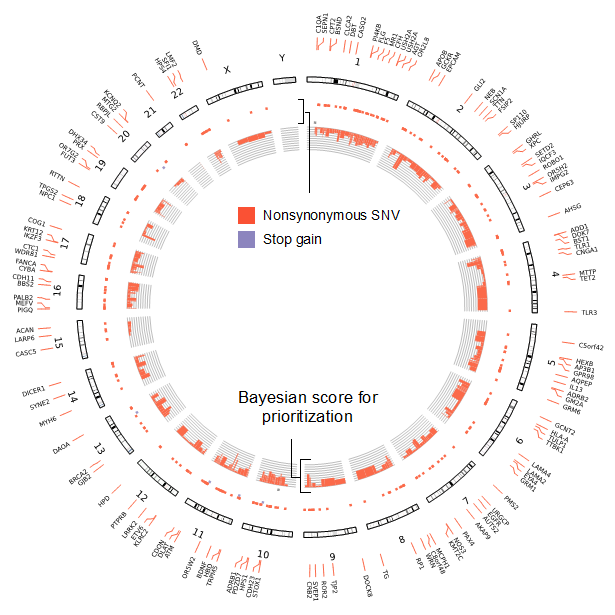
\includegraphics{circosplot.png}
\caption{Circos plot of top 300 ranked genes from Bayesian network ranking. In this Circos plot, the outer track indicates the top ranked genes and their positions on the chromosome. The inner track describes the type of mutation that was observed - most mutations were non-synonymous SNVs, with a few stop-gain mutations. The innermost track shows the relative probabilities of each ranked gene.}
\centering
\end{figure}

\newpage
\section{Discussion}
We demonstrate the validation of high-confidence variant calls using an optimised deep learning neural network on both real and simulated datasets, and we also show that a Bayesian network can rank and prioritise genes in a systematic way so as to obtain important genes. We show that four of the top five genes had published findings that linked them with lymphoma. Looking at the top 300 genes ranked, we also found interesting families of genes that are known to be involved in Lymphoma progression. To benchmark these results, we compared our variant calling results with other methods like VariantMetaCaller(using Support Vector Machines) and BAYSIC(using Bayesian Latent Analysis) (Gézsi et al., 2015; Cantarel et al., 2014), and we also looked at other methods of gene prioritisation to see how our ranking system compares.
\subsection{Comparison of Deep Learning with other Integration Methods}
First, we looked at other methods of integrating variant call information, including VariantMetaCaller, which uses Support Vector Machines (a decision making machine learning technique) and BAYSIC, a method that uses a Bayesian probabilistic model to integrate variant call information. Both methods were also used to analyse and predict variants for NA12878 data (Gézsi et al., 2015), but due to differences in metrics, processes and datasets, absolute comparison of precision and recall is difficult. Thus, it is more suitable to study the looking at relative improvements seen when using each method. VariantMetaCaller increased SNP prediction by 0.04 and indel prediction by 0.07 in terms of the Area Under Prediction Recall Curve (AUPRC) metric when compared to their best single variant caller. The AUPRC measures the precision differences at all levels of recall. BAYSIC also noted a 0.03 increase in SNP prediction and 0.05 increase in indel prediction compared to the best single variant caller. Numerically, this seems comparable to our results of a 0.06 increase in both indel and SNP prediction for the NA dataset compared to the best single variant caller. However, since we used the F1 score metric, instead of the AUPRC metric, an relative quantitative comparison is also not so simple. While the AUPRC metric provides evidence of precision and recall improvements at all levels of threshold (Fawcett et al., 2006), it does not provide evidence for a predictors performance at the best threshold. To measure this, the measurement of the F1 score at the best threshold is required - since it is the F1 score that looks at precision and recall for a specific threshold. Instead, what they have shown is that looking at all thresholds, there is an overall increase in precision and performance, but it is unclear what the improvements are at the optimised thresholds. Fawcett (2006) also mentions this problem, as he notes that 'It is possible for a high-AUC classifier to perform worse in a specific region of ROC space than a low-AUC classifier'. Here, AUC refers to the Area Under Curve, another term for the AUPRC, and ROC refers to the Receiver Operator Characteristics graph (Egan, 1976) which is the curve that the AUPRC uses. Thus, a higher AUPRC does not mean that one caller will outperform another when considering only the optimised threshold.  Measurement of the F1 score is more relevant in clinical practice as we are mainly interested in the optimal operating conditions where precision and recall are maximised and not the fringe conditions. Our results provide specific evidence that at the optimal recall threshold for each specific type of caller, we can show an F1 score improvement of 0.06. \\\\ Thus, one definite step moving forward is to incorporate VariantMetaCaller and BAYSIC into our pipelines as negative controls, and measure using the same dataset and same processes whether deep learning is able to outperform these two methods using the same comparison methods and metrics. Intuitively, we believe that deep learning will be able to edge out improvements as deep learning can form complex representations of the data to learn from that Support Vector Machines are unable to do and ultimately outperform Support Vector Machines in decision problems (LeCun et al., 2015; Schmidhuber, 2015) Furthermore, evidence from our flat and dense network architecture shows that putting all the features in a single vector and using that to performing machine learning might not be the best method as it is difficult to learn features from it. \\\\ However, one large limitation in the overall approach of measuring each of the methods against the NA12878 dataset is that the high confidence calls provided is not the ground truth. Zook et al.(2014) themselves estimate a possible false negative or positive that for every 30 million bases in the NA12878 dataset. This is due to true variants that are not inside the high confidence dataset because of errors in one sequencing machine, or genomic regions that cause all sequencing machines to have similar biases and noise. Hence, this would result in misclassification and wrongly called false negative and false positive results, thus skewing the classification results. To solve this problem, a lot of effort has to be put in to obtain a set of verified truth variants via gold standard Sanger sequencing (Tsiatis et al., 2014), but this might be prohibitively expensive for a large sample of mutations. Still, this would have to be done for us to have a good set of truth variables to test prediction software with before such software can be considered for use in actual treatment and diagnosis. 
\subsection{Analysis of Bayesian Network}
For the Bayesian Network analysis, it is more difficult to numerically benchmark our results for gene prioritisation with current platforms. This is because currently used platforms are qualitative methodologies like gene panels (Olek and Berlin, 2002) or manual literature look-ups of disease-related genes, such as using the ClinVar database. While gene panels work well in a clinical setting, with NGS data it is hoped that as much information about a person's genome as possible can be used in treatment and diagnosis (Meldrum et al., 2011). Using a gene ranking system instead of just looking at a set of implicated genes might allow doctors to find out tease out possible homologs or interacting agents that might be related to the known deleterious genes (perhaps in the gene panel) and integrate that into their treatment and diagnosis.
\subsection{Future Directions}
One interesting extension we would like to move into in the future is to be able to integrate a druggable genome into the network, enabling the prioritisation of genes which have possible candidate drug targets. This method would look up a drug-gene interaction database, for example, DGldb (Griffith et al., 2013), and use the results to inform the importance of a gene. This would enable doctors to notice further possible drug candidates that would work very well on the gene profile of the patient that they might not have considered previously, thus increasing their scope of possible treatment options and augmenting their skills. Other directions in the future include being able to include extra variant callers which will provide it with even more feature data, enabling it to make better predictions. We also hope to build structural variant calling neural networks, as this is a current set of variants that our neural network does not take into account. Finally, we would also like to move everything onto a web interface such that it is accessible for use in terms of both variant validation and gene prioritisation. This would enable easy access to both the validation and prioritisation pipelines. \\\\ Thus, in this paper, we have shown the use of deep learning neural networks to successfully validate variants in both real and simulated datasets. We also show that using a Bayesian network can identify important genes within a lymphoma disease sample. Ultimately, we hope to be able to put these networks to use in a clinical setting to augment treatment and diagnosis of diseases.


\newpage
\section{Appendixes}

\subsection{Neural Network Learning}
Machine learning is underpinned by two key phases, the feed-forward phase and the backpropagation phase. The feedforward phase describes the computation of a prediction, and during this phase, the input features are used to compute the final output prediction. For a simple network below:

\begin{figure}[H]
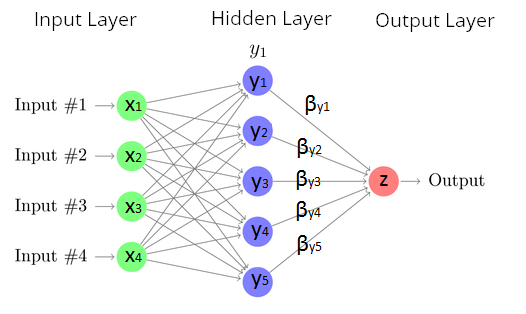
\includegraphics{neuralnetworksample.png}
\caption{Example neural networks with nodes and weights}
\centering
\end{figure}

The final prediction, z is computed with the equation :
\begin{equation}
z = \beta_{y1} * y_1 + \beta_{y2} * y_2 + \beta_{y3} * y_3 + \beta_{y_4} * y_4 + \beta_{y_5} * y_5
\end{equation}
Where $\beta$ indicates the weights linking each output to the input of z and each of the $y_i$ terms are computed in the same manner from the $x_i$ layer. At each node (x,y,z), there is also the existence of an activation function that modifies the input of the node to compute an output. Commonly used activation functions include the rectified linear unit (ReLU), sigmoid functions like hyperbolic tangent and logistic function,$ S(T)=\frac{1}{1+e^{-t}}$.Thus, the final prediction can be seen as a summation of all weights multiplied by the activation output of each node. In theory, we can expand each of the $y_i$ terms in equation (2) to include the $y_i$ layer activation function as well as rewrite the $y_i$ layer inputs in terms of the sum of outputs and weights from the $x_i$ layers. This complex integration of terms allows for the neural network to form complex continuous decision boundaries as the neural networks can compute sophisticated non-linear prediction functions despite being a fundamentally linear model.\\\\ After a prediction is made, we then have to check whether it is correct, and change our weights if an erroneous prediction was made (Figure 24).
\begin{figure}[H]
\centering
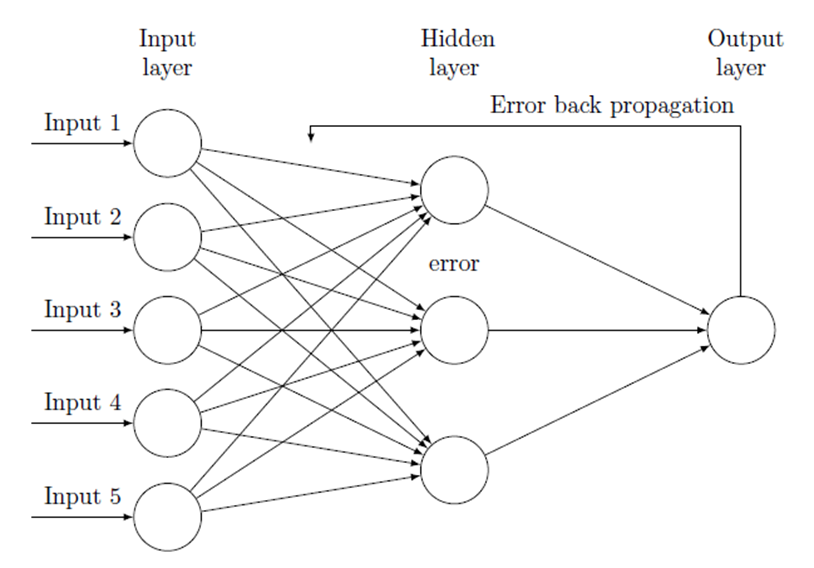
\includegraphics[width=0.8\textwidth]{backpropagation.png}
\caption{Backpropagation of Error Terms}
\end{figure}
This is the backpropagation step, which involves backpropagating the error terms from the output layers to the input layer and updating the weights at each node based on the differential relationship between the error and each specific gradient. Specifically, this is governed by the optimiser functions which have been mentioned earlier - one example of such an function is the Stochastic Gradient Descent function, which is 
\begin{equation}
\beta^n_{yi} = \beta^{n-1}_{yi} - \alpha \frac{\partial{E_n}(\beta)}{\partial{\beta_i}}
\end{equation}
Here, each $\beta$ term indicates a gradient, $\alpha$ is a constant for the learning rate and $\frac{\partial{E_n}(\beta)}{\partial{\beta_i}}$ is the term used to modify the weight of the gradient based on the cost function ${E_n}(\beta)$. The idea used in all backpropagation functions is gradient descent, where the contribution of the gradient term to the error is computed and the gradient is changed by an amount in order to reduce the future contribution of the gradient to that error. Here it is useful to consider what the cost function ${E_n}(\beta)$ is. It is essentially the error rate when a set of gradients is used to perform predictions, as it measures how many accurate predictions were made and how many wrong predictions were made. For a binary class predictor (which is what we are using, only true and false), this is given by the equation
\begin{equation}
E(\beta) = - \frac{1}{n}\sum_{i=1}^{n}{\sum_{j=1}^{2}y_{ij}log(p_{ij})}
\end{equation} 
where $y_{ij}$ indicates the empirical observed probabilities of each class label while $log(p_{ij}$ is the theoretical probabilities of each class label. This is also known as binary cross-entropy, which is derived from Shannon's entropy (See Appendix 5.2.1). From this term, we see that if the neural network predicts something with a high probability ($y_{ij}$ is high) and it is false ($p_{ij}$ is low) so then $log(p_{ij})$ is a big negative number, and so the cost function will very high. On the other hand, if $y_{ij}$ and $p_{ij}$ is high then the entropy will be close to zero, indicating a correct prediction. Since each of the prediction terms can be rewritten in terms of the gradient(rewrite z in terms $\beta y_i $ and so on, we can theoretically compute the contribution of each gradient to the cost function to see how the cost function changes as the gradient changes. Thus, this is what gradient descent does - it tries to see how the cost function changes as each gradient changes, then attempts to move the gradient in the direction that minimises the error term.

\begin{figure}[H]
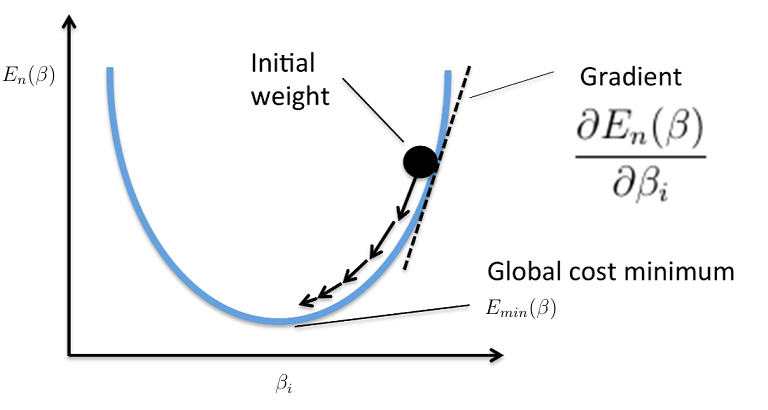
\includegraphics[width=\textwidth]{gradientdescent.png}
\caption{Gradient Descent, which attempts to find the gradient at which the cost function is minimised (since the cost function depends on the gradient).}
\centering
\end{figure}
 This is best seen in Figure 27 above, where the gradient, or specifically the partial differentiation of the cost function with regards to each gradient is used to move the gradient to a new position so as to minimise the error term. Thus, machine learning is in essence a minimisation problem - we want to find a set of weights that minimises the cost function, and because the cost function describes how many predictions we made correctly, this is also training our network to accurately predict outputs from inputs.

\newpage
\subsection{Feature Engineering}
We subset our features into three broad sets, which are base-specific information, sequencing error and bias information features, and calling and mapping quality. \underline{Base information} tells us base specific properties, including information contained in the base as well as the quality of sequenced bases in the samples. \underline{Sequencing error and bias} features attempt to tease out potential biases in sequencing, including features such as GC content, longest homopolymer run and as well as allele balances and counts. Finally, \underline{calling and mapping quality} provides information on the mapping and calling confidence of the variant callers, and includes features such as genotype confidence and mapping quality. In all, these sets of information provide information on the key aspects of variant calling - specifically the properties of the bases in the samples, the characteristics of the sequencing process and finally the variant calling and mapping algorithms.\\\\
\subsubsection{Base Information}
\underline{Shannon Entropy}\\
Shannon Entropy captures the amount of information contained in the allele sequences. It is calculated using the equation :
\begin{equation}
H(X) = -\sum_{i=1}^{n}P(x_i)\log_{2}P(x_i)
\end{equation}
where $P(x_i)$ is the probability of finding each base at each position. Thus, we calculate the entropy by summing up the probabilities/log(probabilities) at each position. This prior probability is calculated in two ways and both are used as features - firstly, the overall genome base probabilities are calculated over the entire genome, and thus the entropy is related to the probability of finding a base at any position in the genome. The second way prior probability is calculated is to take a region of space around the allele (10 bases plus the length of the allele in our calculations) and use those probabilities to calculate the entropy of the allelic sequence. Intuitively, it attempts to find out the amount of information contained within the allelic sequence and hopefully the neural network is able to use the information to determine the validity of a mutation.\\\\
\underline{Kullback Leibler Divergence}\\
The Kullback-Leibler Divergence feature is similar to Shannon entropy, but instead we use this to measure the informational change converting from the reference to the allele sequence. The Kullback-Leibler Divergence is calculated as follows :
\begin{equation}
D_{KL}(P||Q) = -\sum_{i=1}^{n}P(x_i)\log_{2}{\frac{P(x_i)}{Q(x_i)}}
\end{equation}
where $Q(x_i)$ is the prior probability of finding each base at each position based on the genomic region around the allele, while $P(X_i)$ is the posterior probability of finding a specific base inside the allelic sequence. Thus, the KL divergence describes the informational gain when the probabilities from Q is used to describe P. Intuitively, since we know the base probabilities of the region, we can then study the probabilities observed in the reference allelic sequence and see how well $Q(X_i)$ probabilities is able to approximate $P(X_i)$ probabilities.\\\\
\underline{Base Quality}\\
Base quality refers to the Phred score probability that the called allele is wrong. It is given by the equation :
\[ \scalebox{1.2}{$P=10^{\frac{-Q}{10}}$} \]
Where P is the Base Quality and Q is the probability that the allele called is wrong. This is a number computed by the sequencing machine based on the quality of the base samples provided, and tells us how much confidence the sequencing machine has in calling that base.\\\\
\subsubsection{Sequencing Biases and Errors}
\underline{GC content}\\
This feature computes the calculated GC content of reference genome, which may affect sequencing results and accuracy as regions with a GC content are known to be more difficult to sequence. This is because of the greater strength of GC bonds, resulting in errors and biases in sequencing (Benjamini \& Speed, 2012).\\\\ 
\underline{Longest homozygous run}\\
Homopolymer runs (AAAAAAAA) are known to cause sequencer errors (Quail et al.,2012), and might be a factor in determining whether a variant is true. This because long homopolymers provide the same type of signal to the sequencing machine, resulting in a difficult in estimating the magnitude of the signal or rather how many bases are in that homopolymer, resulting in errors and wrongly called variants. The reference sequence region including the allele was checked for homopolymer runs. \\\\
\underline{Allele Count and Allele Balance}\\
Allele count gives the total number of alleles in called phenotypes, while allele balance gives the ratio of final allele called over all other alleles called(reference allele for heterozygous calls, or other alleles for homozygous calls). Both these features give us information of possible biases in the sequencing machine.\\\\
\subsubsection{Calling and Mapping Qualities}
\underline{Genotype Likelihood}\\
The genotype likelihood provides the Phred-scaled likelihood scores of how confident the caller is in determining that it is a homozygous or heterozygous call, and for the homozygous calls whether it is a more likely to be a bi-allelic mutation or no mutation at all. This feature thus gives us the confidence of the caller in determining if one or two alleles have mutated. \\\\ 
\underline{Read Depth}\\
Mapped read depth refers to the total number of bases sequenced and aligned at a given reference base position. The read depth tells us how many reads contributed to a specific call, and thus provides information on how much evidence there is for the variant call\\\\
\underline{Quality by Depth}\\*
Quality by Depth is computed by dividing the quality score against allele depth, to obtain an average score of allele quality. This composite feature provides information on the information provided by each read supporting the call\\\\
\underline{Mapping Quality}\\
Mapping quality is originally a score provided by the alignment method and gives the probability that a read is placed accurately. The variant callers compute a overall mapping quality of the reads that provide evidence for a variant call which is given in this feature. A low mapping quality means that there are multiple positions where the reads contributing to this variant call could have gone, and thus providing evidence that this might not be an accurate call due to poor mapping.\\\\
\newpage
\subsection{Mathematical and Statistical Tools}
\subsubsection{Derivation of F1 Score}
The F1 score is a useful measure as it can measure both the precision as well as the recall of a predictor. For a binary predictor with a binary truth class(Figure 26), we can obtain 4 types of results - true positives, true negatives, false positives and false negatives. 
\begin{figure}[H]
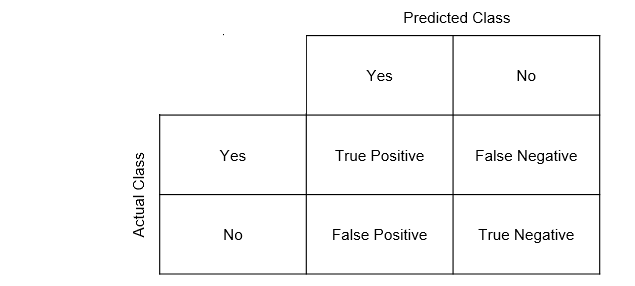
\includegraphics[width=0.8\textwidth]{confusionmatrix.png}
\caption{Confusion Matrix}
\centering
\end{figure}
True positives are positive predictions that are made that are actually positive class labels, while false positives are positive predictions that are made that have negative class labels. Similarly, true negatives are negative predictions that have negative class labels, while false negatives are negative predictions that are actually positive class labels. From this, we can define two equations, precision and recall. Precision is defined as (8) while recall is defined as (9). 
\begin{equation}
Precision = \frac{True \ Positive}{True\  Positive + False \ Positive} 
\end{equation}
\begin{equation}
Recall\ \ \ \ = \frac{True\ Positive}{True \ Positive + False \ Negative} 
\end{equation}
Precision tells us how likely a positive prediction made will be true, while recall tells us how much of the truth class positive predictions the predictor is able to encompass. Thus, a predictor can have a high precision but low recall (makes few predictions but are very accurate) or a high recall and low precision(makes a lot of predictions that capture all truth variables, but have a lot of false positives as well). In genomics, both types of errors are not desired - we would want all the predictions to be true (precision), while not losing out on any important mutations (recall). Thus, we use the composite metric, the F1 score, that looks at the overall precision and recall of a predictor. It is defined as follows :
\begin{equation}
{F1} \ Score \ \ \  \ \ = \frac{2*Precision*Recall}{Precision + Recall} 
\end{equation}
\\
\subsubsection{Principal Components Analysis (PCA)}
Principal Components Analysis (PCA) is a commonly used tool for dimensionality reduction. It was first proposed by Pearson in 1901 (Pearson, 1901) and has been commonplace in many data analytics and signal processing methodologies (Jolliffe, 2002). PCA works by attempting to discover orthogonal principal components (PCs) that are able to represent the original data. Specifically, this means that the PCs are able to capture variance in the datasets. This is done by finding the Eigenvalues and Eigenvectors of the dataset, with the eigenvectors representing a linear combination of all input variables and the eigenvalues representing the amount of variance that that eigenvector is able to represent. Ultimately, we select n eigenvectors that is able to represent a percentage of variance in our dataset. Because each eigenvector is orthogonal, they are able to capture the variance in the dataset. For our analysis, we decided to use 8 principal components - we took the limit as the last principal components that was able to represent at least 0.5\% of variance in the dataset.
 
\begin{figure}[H]
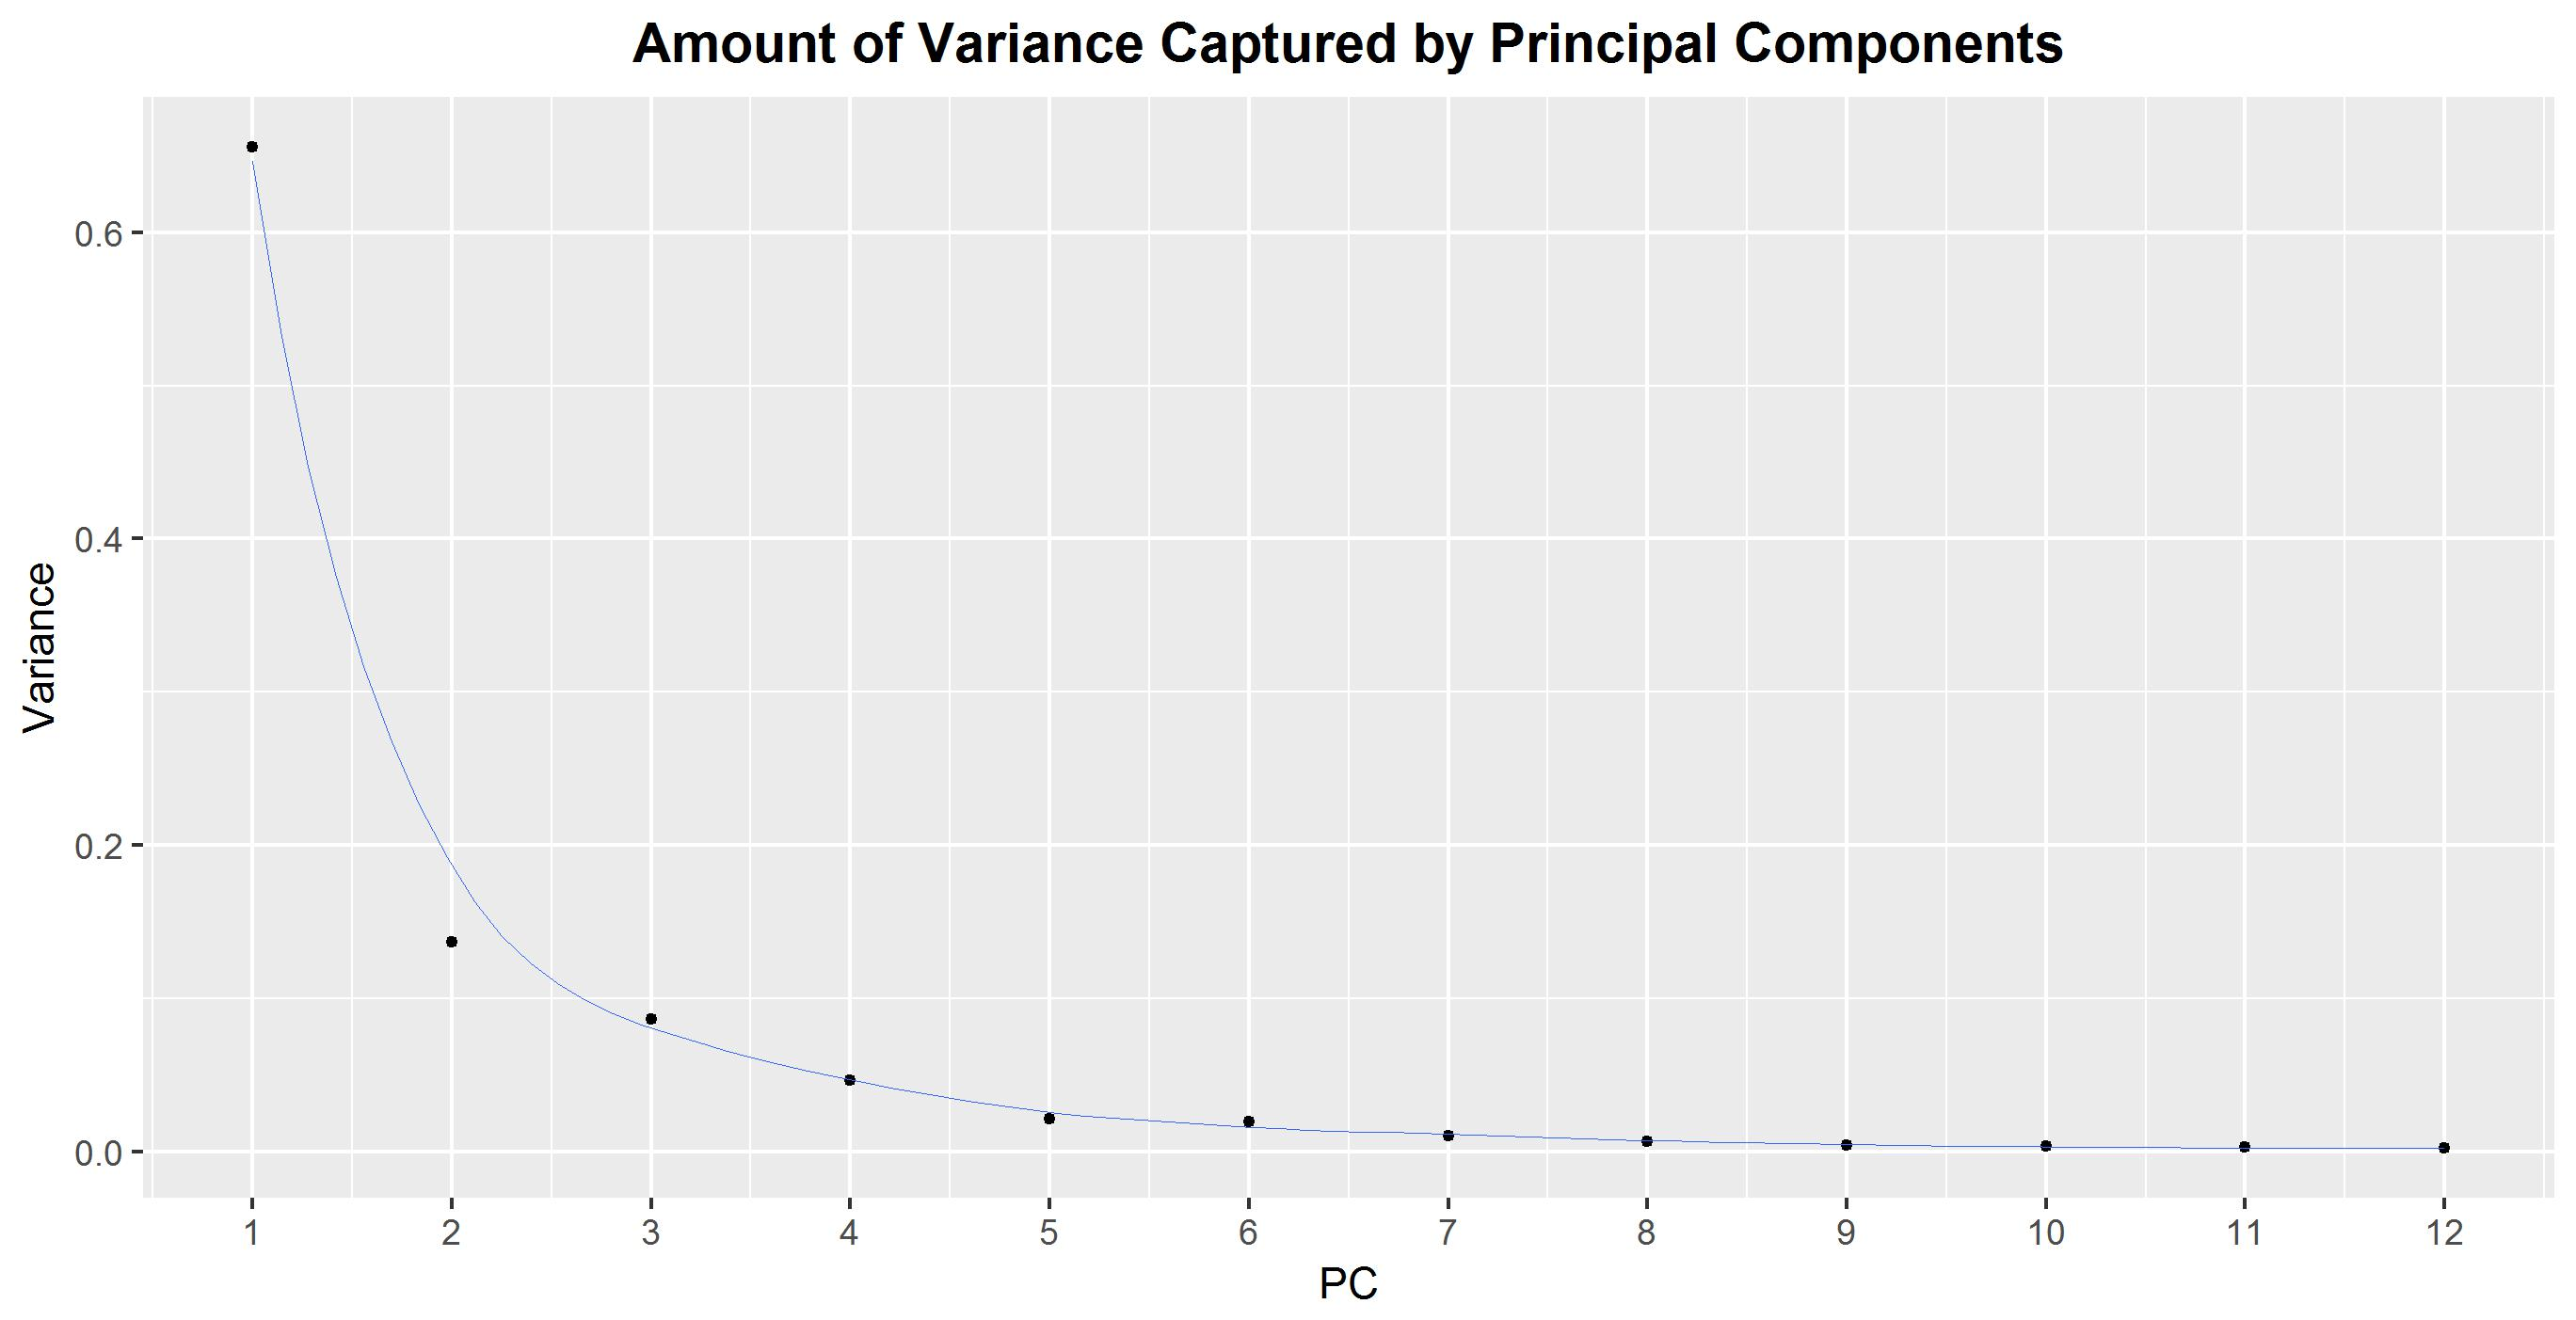
\includegraphics[width=\textwidth]{variancecapturedbypc.jpg}
\caption{Variance captured by first 12 principal components}
\centering
\end{figure}

To carry out PCA, we used the preprocessing step SciPy to normalise all the input vectors to mean 0 and standard deviation 1. Subsequently, we perform principal components decomposition to obtain the eigenvector transformed representation of the dataset and their corresponding eigenvalues. We then fit 8 of the principal components that explained the largest amount of variance into the neural network to study if it can learn from the compressed representation of the input features. 
\subsubsection{Synthetic Minority Overrepresentation Technique (SMOTE)}
SMOTE is a statistical technique described in by Chawla et al. (2002) to overcome problems with imbalanced datasets that are common in machine learning. SMOTE oversamples the training class with fewer variables in a way that tries not to replicate data points (that makes certain data points over-represented) without creating new invalid training examples. It does this by taking the intersection of two nearest data points of the same training class. This can be seen in Figure 28. 

\begin{figure}[H]
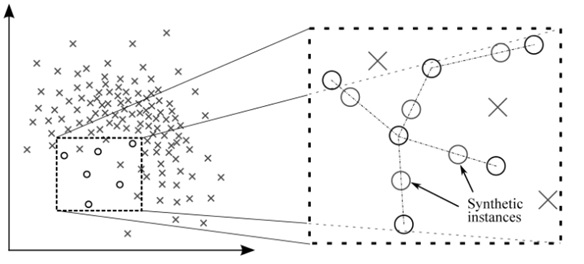
\includegraphics[width=\textwidth]{smoteoversampling.jpg}
\caption{SMOTE oversampling algorithm}
\centering
\end{figure}

In doing so, it creates a more generalised representation of the sample class with less training examples, without replicating certain datapoints and without creating invalid data. This enables intelligent oversampling of the dataset to balance out the positive and negative feature classes. SMOTE has been shown to be valid for other datasets including sentence boundary detection (Liu et al., 2006) and data mining (Chawla, 2005).
\newpage
\section{Bibilography}

\begin{list}{}{%
\setlength{\topsep}{0pt}%
\setlength{\leftmargin}{0.5in}%
\setlength{\listparindent}{-0.5in}%
\setlength{\itemindent}{-0.5in}%
\setlength{\parsep}{\parskip}%
}%
\item[]\item[] Abyzov, A., Li, S., Kim, D. R., Mohiyuddin, M., Sttz, A. M., Parrish, N. F., ... \& Korbel, J. O. \(2015\). Analysis of deletion breakpoints from 1,092 humans reveals details of mutation mechanisms.Nature communications,6.\\\item[] Angrist, M. \(2016\). Personal genomics: Where are we now?.Applied \& translational genomics,8, 1.\\\item[] Chawla, N. V. \(2005\). Data mining for imbalanced datasets: An overview. InData mining and knowledge discovery handbook\(pp. 853-867\). Springer US.\\\item[] Chawla, N. V., Bowyer, K. W., Hall, L. O., \& Kegelmeyer, W. P. \(2002\). SMOTE: synthetic minority over-sampling technique.Journal of artificial intelligence research,16, 321-357.\\\item[] Chen, Y., Lin, Z., Zhao, X., Wang, G., \& Gu, Y. \(2014\). Deep learning-based classification of hyperspectral data. IEEE Journal of Selected topics in applied earth observations and remote sensing, 7\(6\), 2094-2107. Chicago \\\item[] Cornish, A., \& Guda, C. \(2015\). A comparison of variant calling pipelines using genome in a bottle as a reference.BioMed research international,2015.\\\item[] Danecek, P., Auton, A., Abecasis, G., Albers, C. A., Banks, E., DePristo, M. A., ... \& McVean, G. \(2011\). The variant call format and VCFtools.Bioinformatics,27\(15\), 2156-2158.\\\item[] DePristo, M. A., Banks, E., Poplin, R., Garimella, K. V., Maguire, J. R., Hartl, C., ... \& McKenna, A. \(2011\). A framework for variation discovery and genotyping using next-generation DNA sequencing data. Nature genetics, 43\(5\), 491-498.\\\item[] Escalona, M., Rocha, S., \& Posada, D. \(2016\). A comparison of tools for the simulation of genomic next-generation sequencing data.Nature Reviews Genetics,17\(8\), 459-469.\\\item[] Garrison, E., \& Marth, G. \(2012\). Haplotype-based variant detection from short-read sequencing.arXiv preprint arXiv:1207.3907.\\\item[] Garrison, E., \& Marth, G. \(2012\). Haplotype-based variant detection from short-read sequencing.arXiv preprint arXiv:1207.3907.\\\item[] Gzsi, A., Bolgr, B., Marx, P., Sarkozy, P., Szalai, C., \& Antal, P. \(2015\). VariantMetaCaller: automated fusion of variant calling pipelines for quantitative, precision-based filtering. BMC genomics, 16\(1\), 1.\\\item[] Huval, B., Wang, T., Tandon, S., Kiske, J., Song, W., Pazhayampallil, J., ... \& Mujica, F. \(2015\). An empirical evaluation of deep learning on highway driving.arXiv preprint arXiv:1504.01716.\\\item[] Hwang, S., Kim, E., Lee, I., \& Marcotte, E. M. \(2015\). Systematic comparison of variant calling pipelines using gold standard personal exome variants.Scientific reports,5, 17875.\\\item[] Jolliffe, I. \(2002\).Principal component analysis. John Wiley \& Sons, Ltd.\\\item[] Kingma, D., \& Ba, J. \(2014\). Adam: A method for stochastic optimization.arXiv preprint arXiv:1412.6980.\\\item[] LeCun, Y., Bengio, Y., \& Hinton, G. \(2015\). Deep learning.Nature,521\(7553\), 436-444.\\\item[] Li, H., Handsaker, B., Wysoker, A., Fennell, T., Ruan, J., Homer, N., ... \& Durbin, R. \(2009\). The sequence alignment/map format and SAMtools. Bioinformatics, 25\(16\), 2078-2079.\\\item[] Linderman, M. D., Brandt, T., Edelmann, L., Jabado, O., Kasai, Y., Kornreich, R., ... \& Schadt, E. E. \(2014\). Analytical validation of whole exome and whole genome sequencing for clinical applications.BMC medical genomics,7\(1\), 20.\\\item[] Liu, X., Han, S., Wang, Z., Gelernter, J., \& Yang, B. Z. \(2013\). Variant callers for next-generation sequencing data: a comparison study.PloS one,8\(9\), e75619.\\\item[] Liu, Y., Stolcke, A., Shriberg, E., \& Harper, M. \(2005, June\). Using conditional random fields for sentence boundary detection in speech. InProceedings of the 43rd Annual Meeting on Association for Computational Linguistics\(pp. 451-458\). Association for Computational Linguistics.\\\item[] Lpez, V., Fernndez, A., Garca, S., Palade, V., \& Herrera, F. \(2013\). An insight into classification with imbalanced data: Empirical results and current trends on using data intrinsic characteristics.Information Sciences,250, 113-141.\\\item[] Maas, A. L., Hannun, A. Y., \& Ng, A. Y. \(2013, June\). Rectifier nonlinearities improve neural network acoustic models. InProc. ICML\(Vol. 30, No. 1\).\\\item[] McKenna, A., Hanna, M., Banks, E., Sivachenko, A., Cibulskis, K., Kernytsky, A., ... \& DePristo, M. A. \(2010\). The Genome Analysis Toolkit: a MapReduce framework for analyzing next-generation DNA sequencing data.Genome research,20\(9\), 1297-1303.\\\item[] Mohiyuddin, M., Mu, J. C., Li, J., Asadi, N. B., Gerstein, M. B., Abyzov, A., ... \& Lam, H. Y. \(2015\). MetaSV: an accurate and integrative structural-variant caller for next generation sequencing. Bioinformatics, btv204.\\\item[] O'Rawe, J., Jiang, T., Sun, G., Wu, Y., Wang, W., Hu, J., ... \& Wei, Z. \(2013\). Low concordance of multiple variant-calling pipelines: practical implications for exome and genome sequencing.Genome medicine,5\(3\), 1.\\\item[] Pearson, K. \(1901\). Principal components analysis.The London, Edinburgh and Dublin Philosophical Magazine and Journal,6\(2\), 566.\\\item[] Rehm, H. L. \(2017\). Evolving health care through personal genomics.Nature Reviews Genetics.\\\item[] Ruder, S. \(2016\). An overview of gradient descent optimization algorithms.arXiv preprint arXiv:1609.04747.\\\item[] Sandmann, S., de Graaf, A. O., Karimi, M., van der Reijden, B. A., Hellstrm-Lindberg, E., Jansen, J. H., \& Dugas, M. \(2017\). Evaluating Variant Calling Tools for Non-Matched Next-Generation Sequencing Data.Scientific Reports,7.\\\item[] Schirmer, M., DAmore, R., Ijaz, U. Z., Hall, N., \& Quince, C. \(2016\). Illumina error profiles: resolving fine-scale variation in metagenomic sequencing data.BMC bioinformatics,17\(1\), 125.\\\item[] Spencer, D. H., Abel, H. J., Lockwood, C. M., Payton, J. E., Szankasi, P., Kelley, T. W., ... \& Duncavage, E. J. \(2013\). Detection of FLT3 internal tandem duplication in targeted, short-read-length, next-generation sequencing data. The Journal of molecular diagnostics, 15\(1\), 81-93.\\\item[] Srivastava, N., Hinton, G. E., Krizhevsky, A., Sutskever, I., \& Salakhutdinov, R. \(2014\). Dropout: a simple way to prevent neural networks from overfitting. Journal of Machine Learning Research, 15\(1\), 1929-1958.\\\item[] Sutskever, I., Martens, J., Dahl, G. E., \& Hinton, G. E. \(2013\). On the importance of initialization and momentum in deep learning. ICML \(3\), 28, 1139-1147.\\\item[] Talwalkar, A., Liptrap, J., Newcomb, J., Hartl, C., Terhorst, J., Curtis, K., ... \& Patterson, D. \(2014\). SMaSH: a benchmarking toolkit for human genome variant calling.Bioinformatics,30\(19\), 2787-2795.\\\item[] McKenna, A., Hanna, M., Banks, E., Sivachenko, A., Cibulskis, K., Kernytsky, A., ... \& DePristo, M. A. \(2010\). The Genome Analysis Toolkit: a MapReduce framework for analyzing next-generation DNA sequencing data.Genome research,20\(9\), 1297-1303.\\\item[] Tieleman, T. and Hinton, G. Lecture 6.5 - RMSProp, COURSERA: Neural Networks for Machine Learning. Technical report, 2012\\\item[] Van Der Maaten, L., Postma, E., \& Van den Herik, J. \(2009\). Dimensionality reduction: a comparative.J Mach Learn Res,10, 66-71.\\\item[] Xie, M., Lu, C., Wang, J., McLellan, M. D., Johnson, K. J., Wendl, M. C., ... \& Ozenberger, B. A. \(2014\). Age-related mutations associated with clonal hematopoietic expansion and malignancies.Nature medicine,20\(12\), 1472-1478.\\\item[] Yan, Y., Chen, M., Shyu, M. L., \& Chen, S. C. \(2015, December\). Deep learning for imbalanced multimedia data classification. InMultimedia \(ISM\), 2015 IEEE International Symposium on\(pp. 483-488\). IEEE.\\\item[] Ye, K., Schulz, M. H., Long, Q., Apweiler, R., \& Ning, Z. \(2009\). Pindel: a pattern growth approach to detect break points of large deletions and medium sized insertions from paired-end short reads.Bioinformatics,25\(21\), 2865-2871.\\\item[] Zook, J. M., Chapman, B., Wang, J., Mittelman, D., Hofmann, O., Hide, W., \& Salit, M. \(2014\). Integrating human sequence data sets provides a resource of benchmark SNP and indel genotype calls.Nature biotechnology,32\(3\), 246-251.\\


\end{list}

\newgeometry{a4paper, margin=1in}
\newpage
\section{Relevant Code}
3 code segments are provided to clarify the implementation of generating the matrixes for deep learning, deep learning networks and finally bayesian networks. Other code segments not shown include the code base for parsing vcf input into features, concordance generators, NextFlow and Bash code used to simulate and process genomic data as well as to control deep learning and analytic pipelines, and other python helper scripts (e.g. comparing two VCF files, analysis with pre-trained network).
\subsection{generate\_matrixes.py}
\begin{minted}[linenos=true,numberblanklines=true,showspaces=false,breaklines=true,
fontsize=\footnotesize,breakautoindent=true]{python}
#This python script generates the set of matrixes to be used in deep learning, and then calls the main method that trains the deep learning network.
#Input : a directory that contains all the vcf files for processing, as well as a truth file. 
#Output : np.arrays of features from generate_matrixes with accompanying truth labels, feature set lengths, a dictionary of vcf object records, as well as the list of relevant sample features for easy reference
#Notes :
#Vcf files should have the "vcf" string in their name and truth file should have a "truth" string in its name.
#No other file should be present in the folder
#Overall Strategy :
#Generate a dictionary of lists, where the keys are mutations, and the value is contains a matrix containing information of all five callers
#Secondly, for each mutation label, check if it is inside the truth file or not. The truth is preloaded into a dictionary
#Finally, pass the set of features with accompanying truth labels to the neural network 
#The main datastructure used are python dictionaries, which allows O(1) dictionary lookup times 

import os  
import time
from ANNgenerateresults import *  #this file contains all the main methods for actual neural network training
from methods import *  #this file contains all the methods for parsing each VCF entry into a numerical list of features

#declare names of useful files that contains processed data to be saved
LIST_OF_INPUTS_NAME = '/ANN/samplelist.p'     
TRUTH_DICTIONARY_NAME = '/ANN/truthdict.p'
CALLER_LENGTH_FILE_NAME = '/ANN/callerlengths.txt'
VCF_LIST_FILE_NAME = '/ANN/vcf_list.p'
SCORES_NAME = '/ANN/scores.txt'
Y_DATA_NAME = '/ANN/myydata.txt'
X_DATA_NAME = '/ANN/myXdata.txt'

#Initialise NUMBER_OF_CALLERS
NUMBER_OF_CALLERS = 5


# This method follows the typical input output processing pipeline 
# It takes in the user input, and loads it into local variables. 
# It then executes another method, main_analyse_samples_and_truth on the loaded variables
# Finally, it then saves files into a directory determined by the final variables, and calls the next step of the pipeline
# the neural network training, which is main_gather_input_execute_prep_output

def load_and_save_data(user_input):
    user_input = vars(user_input)   
    input_samples, referencepath, output_location = load_references(user_input)   # load user input
    my_x_dataset, my_y_dataset, list_of_samples, truth_dictionary, length_of_caller_outputs, \
    vcf_record_list = main_analyse_samples_and_truth(input_samples, referencepath) 
    save_files(output_location, my_x_dataset, length_of_caller_outputs,
               list_of_samples, truth_dictionary, vcf_record_list, my_y_dataset) 
    orig_stdout = sys.stdout  #save print statements into stdout
    f = file(str(output_location) + SCORES_NAME, 'w')
    sys.stdout = f
    main_gather_input_execute_prep_output(length_of_caller_outputs, truth_dictionary, my_x_dataset, my_y_dataset, list_of_samples, output_location, vcf_record_list) 

# This method first prepares a dictionary of truth to be checked against. It then initialises
# a dictionary of samples with all the keys, each key being a variant call, and then fills it up each key with data from each caller
# subsequently, it removes dictionary entries that are the wrong size, and then checks whether
# each entry in the dictionary is true or not by looking up the truth dictionary
# subsequently it performs array balancing, and converts the data to np.array, as well as the dictionary of truth
# and list of called samples

def main_analyse_samples_and_truth(path, referencepath):
    os.chdir(path)
    truthdict = generate_truth_list(path)       
    print "truth dictionary generated at time :", time.time() - start
    callerlengths, list_of_called_samples, vcf_list = generate_input(path, referencepath)
    print "samples generated at time :", time.time() - start
    clean_truth_array, cleaned_sample_array = check_predicted_with_truth(list_of_called_samples, truthdict)
    print "samples checked with truth at time :", time.time() - start
    cleaned_sample_array = np.array(cleaned_sample_array, np.float64)
    clean_truth_array = np.array(clean_truth_array)
    return cleaned_sample_array, clean_truth_array, list_of_called_samples, truthdict, callerlengths, vcf_list

# This method generates the truth dictionary, by iterating through the vcf file, parsing all the vcf entries and appending them all as keys in the dictionary 

def create_truth_dictionary(generated_truth_dictionary, truth_file):
    vcf_reader = vcf.Reader(open(truth_file, 'r'))    
    for record in vcf_reader:
        if "GL" in record.CHROM:    #Ignore non-regular chromosomes in our dataset
            continue
        templist = []
        for item in record.ALT:
            templist.append(str(item).upper())          #Alternates might be a list, so they have to be saved as a immutable tuple
        generated_truth_dictionary[(str(record.CHROM), str(record.POS), str(record.REF).upper())] = tuple(templist)

# This method generates the input dictionary, by first initialising the keys of the dictionary by iterating through the vcf file once, and then
# Iterating through the vcf file again and parsing all the entries as input vectors

def generate_input(path, referencepath):
    reference_dictionary = get_reference_dictionary_for_entropy(referencepath)
    base_entropy = get_ref_entropy(referencepath)
    full_dictionary = get_dictionary_keys(path)
    list_of_called_samples, callerlengths, vcf_list = fill_sample_dictionary(base_entropy, full_dictionary, path, reference_dictionary)
    return callerlengths, list_of_called_samples, vcf_list


# This method goes through all the training variant calling files and extracts unique calls as keys in the sample dictionary

def get_dictionary_keys(path):
    sample_dictionary = {}
    for vcf_file in os.listdir(path):
        if ignore_file(vcf_file):
            continue
        vcf_reader = vcf.Reader(open(vcf_file, 'r'))
        sample_dictionary = create_dictionary_keys(vcf_reader, sample_dictionary)
    return sample_dictionary

#This method ensures the feature vector is in the right order - the entries must always be in the order fb, hc, ug, pindel and st.

def create_list_of_paths(path):
    list_of_paths = [0] * NUMBER_OF_CALLERS
    for vcf_file in os.listdir(path):
        if ignore_file(vcf_file):
            continue
        if "fb" in vcf_file:
            list_of_paths[0] = vcf_file
        if "hc" in vcf_file:
            list_of_paths[1] = vcf_file
        if "ug" in vcf_file:
            list_of_paths[2] = vcf_file
        if "pind" in vcf_file:
            list_of_paths[3] = vcf_file
        if "st" in vcf_file:
            list_of_paths[4] = vcf_file
    return list_of_paths

# This method goes through all the training variant calling files and fills each entry in a sample dictionary
# with data. If it is empty, it returns an array of length n, where n is the number of variables
# that same caller would have provided.
# Each caller has a different amount of variables because it contains different datasets

def fill_sample_dictionary(base_entropy, sample_dictionary, path, reference_dictionary):
    callerlengths = [0] * number_of_callers
    index = 0
    total_mode_value = 0
    list_of_paths = create_list_of_paths(path)
    for vcf_file in list_of_paths:
        index += 1
        opened_vcf_file = vcf.Reader(open(vcf_file, 'r'))
        removaldict = iterate_over_file_to_extract_data(base_entropy, sample_dictionary,
                                                        reference_dictionary, opened_vcf_file, vcf_file)
        mode_value = get_mode_value(removaldict)
        add_length_to_caller_lengths_based_on_file_name(vcf_file, mode_value, callerlengths)
        refill_dictionary_with_zero_arrays_for_each_file(sample_dictionary, index, mode_value)
        total_mode_value += mode_value
    list_of_passed_samples, vcf_list = add_mode_values_into_list_of_samples(sample_dictionary, total_mode_value)
    return list_of_passed_samples, callerlengths, vcf_list


# this method fills the dictionary with empty arrays with the same length as the ones that were supposed to be added

def refill_dictionary_with_zero_arrays_for_each_file(full_dictionary, index, length_of_data_array):
    empty_set = []
    for i in range(length_of_data_array):
        empty_set.append(0)
    for item in full_dictionary:
        checksum = len(full_dictionary[item][0])
        if checksum < index:
            arbinfo = empty_set
            full_dictionary[item][0].append(arbinfo)


# this method iterates through all the files to extract data from each sample. It uses methods from the
# methods.py function, which parses each record for data.

def iterate_over_file_to_extract_data(base_entropy, sample_dictionary, recorddictionary, vcf_reader1, vcf_file):
    removaldict = {}
    for record in vcf_reader1:
        if "GL" in str(record.CHROM):
            continue
        sample_name = get_sample_name_from_record(record)
        sample_data = getallvalues(record, recorddictionary, base_entropy, vcf_file)
        sample_dictionary[sample_name][0].append(sample_data)
        sample_dictionary[sample_name][1] = record
        create_removal_dict(sample_data, removaldict)
    return removaldict

# this method counts the mode number of entries in the dictionary. Due to certain vcf files having multiple possible number of entries for a field, this will create an error
# as the size of the input arrays should always be constant. Thus, any sample that does not fit the array should be removed. 
# TO-DO See if a better implementation can be done that doesn't reduce data available
	
def create_removal_dict(sample_data, removaldict):
    count = 0
    count += len(sample_data)
    if count not in removaldict:
        removaldict[count] = 1
    else:
        removaldict[count] += 1


# this method prepares the reference genome dictionary for use in entropy calculations

def get_reference_dictionary_for_entropy(reference_path):
    record_dictionary = SeqIO.to_dict(SeqIO.parse(reference_path, "fasta"), key_function=get_chr)
    return record_dictionary

# this method ensures that the files inputed are correct

def ignore_file(vcf_file):
    if "vcf" not in vcf_file or "truth" in vcf_file:
        return True
    return False

# this method creates the set of keys for the dictionary
	
def create_dictionary_keys(vcf_reader, sample_dictionary):
    for record in vcf_reader:
        if "GL" in str(record.CHROM):
            continue
        sample_name = get_sample_name_from_record(record)
        sample_dictionary[sample_name] = [[], []]  # fullname has become a key in fulldictionary
    return sample_dictionary

# standard method that returns a tuple of the variant call object with the chromosome, position, reference and tuple of alternates

def get_sample_name_from_record(record):
    templist = []
    for item in record.ALT:
        templist.append(str(item).upper())
    sample_name = (str(record.CHROM), str(record.POS), str(record.REF).upper(), tuple(templist))
    return sample_name

# this method sets the length of the input neural networks
	
def add_length_to_caller_lengths_based_on_file_name(vcf_file, caller_length, callerlengths):
    if "fb" in vcf_file:
        callerlengths[0] = caller_length
    if "hc" in vcf_file:
        callerlengths[1] = caller_length
    if "ug" in vcf_file:
        callerlengths[2] = caller_length
    if "pind" in vcf_file:
        callerlengths[3] = caller_length
    if "st" in vcf_file:
        callerlengths[4] = caller_length

# this method wraps the create truth dictionary method and is used to checking that the dictionary file has the correct name
		
def generate_truth_list(path):
    generated_truth_dictionary = {}
    for truth_file in os.listdir(path):
        if "truth" not in truth_file:
            continue
        create_truth_dictionary(generated_truth_dictionary, truth_file)
    return generated_truth_dictionary

# this method takes in the mutation (in a tuple) and checks if that mutation exists in the truth dictionary
# A mutation exists if the chromosome, reference and position of the variant call is correct, AND one of the alternate alleles it contains
# is also an alternate allele in the truth dataset
	
def check_sample_against_truth_dictionary(tuple_name, final_truth_list, truth_dictionary):
    temp_tuple = (tuple_name[0], tuple_name[1], tuple_name[2])
    if temp_tuple in truth_dictionary:
        for alternate in tuple_name[3]:
            if alternate in truth_dictionary[temp_tuple]:
                final_truth_list.append(1)
                return
    final_truth_list.append(0)
    return

# This method loads the paths of the files into local variables

def load_references(user_input):
    file1 = user_input['input'][0]
    referencepath = user_input['reference']
    output_location = user_input['output']
    return file1, referencepath, output_location

# This method saves all the processed data into files that can be used for other purposes later or loaded natively instead of doing the processing again

def save_files(output_location, x_array, length_of_caller_outputs, sample_list, truth_dict, vcf_dictionary_file,
               y_array=[]):
    file2 = output_location
    x_data_file_name = str(file2) + str(X_DATA_NAME)
    np.save(x_data_file_name, x_array)
    vcf_file_name = str(file2) + str(VCF_LIST_FILE_NAME)
    caller_length_file_name = str(file2) + str(CALLER_LENGTH_FILE_NAME)
    truth_dictionary_name = str(file2) + str(TRUTH_DICTIONARY_NAME)
    list_of_inputs_name = str(file2) + str(LIST_OF_INPUTS_NAME)
    np.save(caller_length_file_name, length_of_caller_outputs)
    with open(list_of_inputs_name, 'wb') as samplesave1:
        pickle.dump(sample_list, samplesave1)
    with open(truth_dictionary_name, 'wb') as samplesave2:
        pickle.dump(truth_dict, samplesave2)
    with open(vcf_file_name, 'wb') as samplesave3:
        pickle.dump(vcf_dictionary_file, samplesave3)
    if y_array != []:
        y_data_file_name = str(file2) + str(Y_DATA_NAME)
        np.save(y_data_file_name, y_array)

# This method takes in two dictionaries, a dictionary of truth mutations and a dictionary of sample mutations, 
# checks whether each of the sample variables are inside the truth dictionary
# and returns 2 arrays, an array of samples and an array of accompanying truth labels
		
def check_predicted_with_truth(passed_list_of_samples, dictionary_of_truth=[]):
    final_array_of_samples = []
    final_truth_list = []
    for item in passed_list_of_samples:
        if dictionary_of_truth:
            check_sample_against_truth_dictionary(item[0], final_truth_list, dictionary_of_truth)
        temp_array = []
        for row in item[1]:
            temp_array.extend(row)
        final_array_of_samples.append(temp_array)
    if dictionary_of_truth:
        return final_truth_list, final_array_of_samples
    return final_array_of_samples

# This method ensures that only the variables that have the modal number of features are used 
# in neural network training to ensure all array sizes are the same

def add_mode_values_into_list_of_samples(full_dictionary, mode_value):
    list_of_passed_samples = []
    vcf_list = []
    for key in full_dictionary:
        second_count = 0
        for item in full_dictionary[key][0]:
            second_count += len(item)
        if second_count != mode_value:
            continue
        list_of_passed_samples.append([key, full_dictionary[key][0]])
        vcf_list.append(full_dictionary[key][1])
    return list_of_passed_samples, vcf_list

# This method gets the modal number of features from a modal dictionary

def get_mode_value(removaldict):
    curr = 0
    mode_value = 0
    for new_key in removaldict:
        if removaldict[new_key] > curr:
            curr = removaldict[new_key]
            mode_value = new_key
    return mode_value

# This method iterates through the dataset to create a modal dictionary which contains a key-value pair of (number of features - number of times seen).
# The mode number of features is kept
	
def iterate_through_dictionary_to_find_mode_size(full_dictionary):
    removaldict = {}
    samples = 0
    for key in full_dictionary:
        samples += 1
        if samples == sample_limit:
            break
        count = 0
        for item in full_dictionary[key]:
            count += len(item)
        if count not in removaldict:
            removaldict[count] = 1
        else:
            removaldict[count] += 1
    return removaldict


if __name__ == "__main__":
    np.seterr(divide='raise', invalid='raise')
    parser = argparse.ArgumentParser(description="train neural net")
    parser.add_argument('-i', '--input', help="give directories with files", nargs='+')
    parser.add_argument('-d', '--debug', help="look at matrixes built")
    parser.add_argument('-r', '--reference', help="")
    parser.add_argument('-o', '--output', help="")
    paths = parser.parse_args()
    start = time.time()
    load_and_save_data(paths)                              
\end{minted}
\subsection{train\_network.py}

\begin{minted}[linenos=true,numberblanklines=true,showspaces=false,breaklines=true,
fontsize=\footnotesize,breakautoindent=true]{python}
#This script is called by the generate_matrixes.py script and contains the implementation of the neural network.
#Input : np.arrays of features from generate_matrixes with accompanying truth labels, feature set lengths, a dictionary of vcf object records, as well as the list of sample features 
#Output : A VCF file containing all the filtered entries by the neural network, as well the list of accompanying scores 
#Overall Strategy :
#Perform SMOTE oversampling of the input features, and then use the features to train the neural network
#After training, perform validation on test dataset, and subsequently prepare a vcf file with filtered entries


#import all necessary components 
import argparse
import cPickle as pickle
import sys
import numpy as np
import vcf
from imblearn.over_sampling import SMOTE
from keras.callbacks import *
from keras.layers import Dense, Dropout, Activation
from keras.layers.advanced_activations import LeakyReLU
from keras.layers.normalization import BatchNormalization
from keras.models import Sequential
from keras.models import load_model
from keras.optimizers import RMSprop
from sklearn.metrics import *
from sklearn.model_selection import train_test_split


#set constants
PCA_COMPONENTS = 8
STEP_INCREMENT = 10
RECURSION_LIMIT = 0.0002
VERBOSE = 1
seed = 1337

# Initialise random seed for reproducibility
np.random.seed(seed) 

#Prepare file names for saving
vcf_file_name = "/ANN/truevcf.vcf"
keras_model_name = "/ANN/model"
model_truth_name = "/ANN/modeltruths.txt"
model_predictions_name = "/ANN/modelpredictions.txt"
original_vcf_reader = "/data/backup/metacaller/stage/data/version6.3a/hc.vcf.normalisedtrain.vcf"

# this method takes in a path and returns training matrixes for the ANN
# The path should contain n caller vcf files and 1 truth file
# vcf files should be labelled with vcf and truth file should be labelled with truth
# no other file should be present in the folder
def main_gather_input_execute_prep_output(array_sizes, dict_of_truth_input, fullmatrix_sample, fullmatrix_truth, list_of_samples_input, save_location, vcf_dictionary):
    calculated_prediction_actual, calculated_truth_actual = train_neural_net(20, 10, fullmatrix_sample, fullmatrix_truth,                                                                             save_location, array_sizes)
    get_all_relevant_scores(calculated_prediction_actual, calculated_truth_actual, dict_of_truth_input, list_of_samples_input, vcf_dictionary, save_location)

# This method counts the number of false negatives inside the input sample

def count_false_negative(calculated_prediction_actual, calculated_truth_actual):
    count_false_negative = 0
    for i in range(len(calculated_prediction_actual)):
        if calculated_prediction_actual[i] == 0 and calculated_truth_actual[i] == 1:
            count_false_negative += 1
    return count_false_negative

# this is the wrapper function for the recursive hill climbing algorithm to get the best f1 score
# It starts from a low threshold value, and marginally increases the threshold until it is unable to find
# any better F1 scores. It then reports the threshold, F1 score and produces the filtered callset 

def get_all_relevant_scores(calculated_prediction_actual, calculated_truth_actual, dict_of_truth_input,
                            list_of_samples_input, vcf_list, outputpath):
    print "Here are some predictions", calculated_prediction_actual[:100]
    print "here are some truths", calculated_prediction_actual[:100]
    f1_score_left = get_scores(calculated_prediction_actual, calculated_truth_actual, 0.0, list_of_samples_input, dict_of_truth_input)
    guess_f1_final_score, guess_f1_final = recursive_best_f1_score(calculated_prediction_actual,   calculated_truth_actual, dict_of_truth_input, list_of_samples_input, 0.0, f1_score_left, 0.2)
    get_scores(calculated_prediction_actual, calculated_truth_actual, guess_f1_final, list_of_samples_input, dict_of_truth_input, VERBOSE)
    produce_vcf_file(calculated_prediction_actual, guess_f1_final, list_of_samples_input, vcf_list, outputpath)

# This method produces the vcf file through filtering with the neural network threshold calls

def produce_vcf_file(calculated_prediction_actual, guess_f1_final, list_of_samples_input, vcf_list, outputpath):
    prediction = []
    for item in calculated_prediction_actual:
        if item > guess_f1_final:
            prediction.append(1)
        else:
            prediction.append(0)
    list_of_records = []
    for i in range(len(list_of_samples_input)):
        if prediction[i] == 1:
            list_of_records.append(vcf_list[i])
    vcf_reader = vcf.Reader(filename=original_vcf_reader)
    vcf_writer = vcf.Writer(open(outputpath + vcf_file_name, 'w'), vcf_reader)
    for record in list_of_records:
        vcf_writer.write_record(record)

# This method is the recursive function that attempts to find the threshold that produces the best f1 score. It does this
# by iterating through steps of thresholds (0.2, 0.02 and 0.002) until no better F1 score can be found for a marginal increase in threshold. 
# It then returns the best F1 score and the threshold

def recursive_best_f1_score(calculated_prediction_actual, calculated_truth_actual, dict_of_truth_input,
                            list_of_samples_input, guess, guess_score, step):
    if step <= RECURSION_LIMIT:
        return guess_score, guess
    new_guess = guess + step
    new_guess_score = get_scores(calculated_prediction_actual, calculated_truth_actual, new_guess,
                                 list_of_samples_input, dict_of_truth_input)
    if new_guess_score > guess_score:
        return recursive_best_f1_score(calculated_prediction_actual, calculated_truth_actual, dict_of_truth_input,
                                       list_of_samples_input, new_guess, new_guess_score, step)
    return recursive_best_f1_score(calculated_prediction_actual, calculated_truth_actual, dict_of_truth_input,
                                   list_of_samples_input, guess, guess_score, step / STEP_INCREMENT)

# this method uses pre-loaded data to train the neural network. It is optional and only used when this python script is called natively and not imported

def load_references(input_paths):
    input_paths = vars(input_paths)
    fullmatrix_sample = np.load(input_paths['input'][0])
    fullmatrix_truth = np.load(input_paths['input'][1])
    with open(input_paths['input'][3], 'rb') as fp1:
        list_of_samples_input = pickle.load(fp1)
    with open(input_paths['input'][4], 'rb') as fp2:
        dict_of_truth_input = pickle.load(fp2)
    array_sizes = np.load(input_paths['input'][5])
    with open(input_paths['input'][6], 'rb') as fp3:
        vcf_dictionary = pickle.load(fp3)
    orig_stdout = sys.stdout
    f = file(str(input_paths['input'][3]) + '.txt', 'w')
    sys.stdout = f
    return array_sizes, dict_of_truth_input, fullmatrix_sample, fullmatrix_truth, list_of_samples_input, input_paths, vcf_dictionary

# this method solves the double false negative problem that is created due to the neural network prediction scheme
	
def remove_duplicated_false_negative(prediction_list, truth_list, false_negatives):
    count = 0
    removal_list = []
    for i in range(len(prediction_list) - 1, -1, -1):
        if count == false_negatives:
            break
        if prediction_list[i] == 0 and truth_list[i] == 1:
            removal_list.insert(0, i)
            count += 1
    for index in removal_list:
        prediction_list.pop(index)
        truth_list.pop(index)
    return prediction_list, truth_list

# this method takes in the binary truth and predicted samples and calculates the true positive rate, false positive rate, recall, precision and f1 score
	
def get_scores(actual_predictions, actual_truth, value, sample_list, truth_dictionary, verbose=0):
    temp_actual_truth = list(actual_truth)
    prediction = []
    for item in actual_predictions:
        if item > value:
            prediction.append(1)
        else:
            prediction.append(0)
    false_negatives = count_false_negative(actual_predictions, actual_truth)
    finalpredictionnumbers, finaltruthnumbers = add_negative_data(sample_list, truth_dictionary, prediction, temp_actual_truth)
    finalpredictionnumbers, finaltruthnumbers = remove_duplicated_false_negative(finalpredictionnumbers, finaltruthnumbers, false_negatives)
    final_f1_score = f1_score(finaltruthnumbers, finalpredictionnumbers)
    if verbose:
        print_scores(actual_truth, final_f1_score, finalpredictionnumbers, finaltruthnumbers, prediction, value)
    return final_f1_score

# default method for printing all relevant scores
	
def print_scores(actual_truth, final_f1_score, finalpredictionnumbers, finaltruthnumbers, prediction, value):
    final_false_positive, final_true_negative = perf_measure(finaltruthnumbers, finalpredictionnumbers)
    print "final false positive rate is :", final_false_positive
    print "final true negative rate is :", final_true_negative
    print "final precision score is :", precision_score(finaltruthnumbers, finalpredictionnumbers)
    print "final recall score is :", recall_score(finaltruthnumbers, finalpredictionnumbers)
    print "threshold is", value
    print "final F1 score is : ", final_f1_score

# This method looks at the set of predicted samples and the set of truths and adds the false negatives to the predicted sample.
	
def add_negative_data(list_of_samples, dict_of_truth, array_of_predicted, array_of_truth):
    dict_of_samples = generate_sample_dictionary(array_of_predicted, list_of_samples)
    list_of_truth = generate_list_of_truth(dict_of_truth)
    new_array_of_predicted = list(array_of_predicted)
    new_array_of_truth = list(array_of_truth)
    original_length = len(new_array_of_predicted)
    for item in list_of_truth:
        fillnegative(item, dict_of_samples, new_array_of_predicted, new_array_of_truth)
    print "number of false data samples are", (len(new_array_of_predicted) - original_length)
    return new_array_of_predicted, new_array_of_truth

# This method generates a list of truth variant calls from a dictionary of truth variant calls.

def generate_list_of_truth(dict_of_truth):
    list_of_truth = []
    for key in dict_of_truth:
        mytuple = dict_of_truth[key]
        temptuple = []
        for item in mytuple:
            temptuple.append(item)
        list_of_truth.append([key[0], key[1], key[2], temptuple])
    return list_of_truth

# This method generates a dictionary of sample variant calls from a list of sample variant calls.
	
def generate_sample_dictionary(array_of_predicted, list_of_samples):
    dict_of_samples = {}
    for i in range(len(list_of_samples)):
        item = list_of_samples[i]
        if array_of_predicted[i] == 0:
            continue
        new_key = (item[0][0], item[0][1], item[0][2])
        new_value = item[0][3]
        if new_key not in dict_of_samples:
            dict_of_samples[new_key] = new_value
        else:
            dict_of_samples[new_key] = list(dict_of_samples[new_key])
            dict_of_samples[new_key].extend(new_value)
            dict_of_samples[new_key] = tuple(dict_of_samples[new_key])
            # print dict_of_samples[new_key]
    return dict_of_samples

# Actual method to calculated false positive, false negative rates
	
def perf_measure(y_actual, y_hat):
    true_positive = 0
    false_positive = 0
    false_negative = 0
    true_negative = 0

    for i in range(len(y_hat)):
        if y_actual[i] == 1 and y_hat[i] == 1:
            true_positive += 1
    for i in range(len(y_hat)):
        if y_hat[i] == 1 and y_actual[i] == 0:
            false_positive += 1
    for i in range(len(y_hat)):
        if y_actual[i] == 1 and y_hat[i] == 0:
            false_negative += 1
    for i in range(len(y_hat)):
        if y_hat[i] == 0 and y_actual[i] == 0:
            true_negative += 1

    print "true positives :", true_positive
    print "false positives :", false_positive
    print "false negatives :", false_negative
    print "true negatives :", true_negative

    true_positive = float(true_positive)
    false_positive = float(false_positive)
    false_negative = float(false_negative)
    if false_positive == 0 and true_positive == 0:
        false_positive_rate = 0
    else:
        false_positive_rate = false_positive / (false_positive + true_positive)
    if false_negative == 0 and true_positive == 0:
        true_negative_rate = 0
    else:
        true_negative_rate = false_negative / (false_negative + true_positive)

    return false_positive_rate, true_negative_rate


# comparator method that takes a tuple and checks whether it is in the dictionary of samples, if it is not, then add a false negative call to the dataset
	
def fillnegative(tuple1, sampledict, arrayofsamples, arrayoftruths):
    tuple2 = (tuple1[0], tuple1[1], tuple1[2])
    if tuple2 in sampledict:
        for ALT in tuple1[3]:
            if ALT in sampledict[tuple2]:
                return
    arrayofsamples.append(0)
    arrayoftruths.append(1)

# main method that performs neural network training. This method takes in the sample matrixes, the truth variables, a save file location, number of epochs, 
# size of input arrays and the minibatch training size. It first performs SMOTE on the input dataset, then splits it into training and test dataset. It then
# initialises the deep learning layers, compiles the neural network and uses the input data to fit the network. The best set of weights at any point is saved
# to a file and reloaded at the end of the fitting. After training, the neural network is used to predict the original un-oversampled dataset
	
def train_neural_net(mybatch_size, mynb_epoch, myX_train, myy_train, location, arraysize):
    fb_size, hc_size, ug_size, pindel_size, st_size = get_sizes(array_sizes)
    X_resampled, y_resampled = do_smote_resampling(myX_train, myy_train)
    X_train, X_test, y_train, y_test = train_test_split(X_resampled, y_resampled,
                                                        test_size=0.33, random_state=seed)
    X_fb, X_hc, X_ug, X_pindel, X_st = prep_input_samples(array_sizes, X_train)
    X_fb_test, X_hc_test, X_ug_test, X_pindel_test, X_st_test = prep_input_samples(array_sizes, X_test)
    batch_size = mybatch_size
    nb_epoch = mynb_epoch

    fb_branch = Sequential()
    develop_first_layer_matrixes(fb_branch, fb_size)

    hc_branch = Sequential()
    develop_first_layer_matrixes(hc_branch, hc_size)

    ug_branch = Sequential()
    develop_first_layer_matrixes(ug_branch, ug_size)

    pindel_branch = Sequential()
    develop_first_layer_matrixes(pindel_branch, pindel_size)

    st_branch = Sequential()
    develop_first_layer_matrixes(st_branch, st_size)

    final_model = Sequential()
    final_model.add(Merge([fb_branch, hc_branch, ug_branch, pindel_branch, st_branch], mode='concat', concat_axis=1))
    final_model.add(Dense(24, activation='linear'))
    final_model.add(LeakyReLU(alpha=0.05))
    final_model.add(Dense(6, activation='linear'))
    final_model.add(LeakyReLU(alpha=0.05))
    final_model.add(Dense(1, activation='linear'))
    final_model.add(Activation('sigmoid'))
    print (final_model.summary())
    adam = Adam(lr=0.00001, rho=0.9, epsilon=1e-08, decay=0.0)
    final_model.compile(loss='binary_crossentropy',
                        optimizer=adam,
                        metrics=['accuracy'])

    filepath = location + "/best_weights.hdf5"
    checkpoint = ModelCheckpoint(filepath, monitor='val_acc', verbose=1, save_best_only=True, mode='max')
    callbacks_list = [checkpoint]
    model_history = final_model.fit([X_train], y_train, batch_size=batch_size, nb_epoch=nb_epoch,
                                    validation_split=0.2, verbose=2, callbacks=callbacks_list)
    final_model = load_model(location + "/best_weights.hdf5")
    print model_history.history['val_acc'], model_history.history['val_acc']
    print model_history.history['val_loss'], model_history.history['val_loss']
    np.save(location + "/best_weights.hdf5", model_history.history['val_acc'])
    np.save(location + "/best_weights.hdf5", model_history.history['val_loss'])
    scores = final_model.evaluate([X_test], y_test)
    print scores
    final_prediction_array_probabilities = final_model.predict([myX_train])
    final_prediction_array_probabilities = np.squeeze(final_prediction_array_probabilities)
    save_model_details(final_model, final_prediction_array_probabilities, myy_train, location)

    return final_prediction_array_probabilities, myy_train

# Method to perform SMOTE oversampling

def do_smote_resampling(myX_train, myy_train):
    sm = SMOTE(kind='regular')
    where_are_NaNs = np.isnan(myX_train)
    myX_train[where_are_NaNs] = 0
    X_resampled, y_resampled = sm.fit_sample(myX_train, myy_train)
    return X_resampled, y_resampled

# this method saves the details of the neural network

def save_model_details(final_model, save_model_probabilities, trutharray, location):
    name1 = location + model_predictions_name
    name2 = location + model_truth_name
    name3 = location + keras_model_name
    np.save(name1, save_model_probabilities)
    np.save(name2, trutharray)
    final_model.save(name3)

# this method gets the array size of the features used

def get_sizes(array_sizes):
    fb_size = array_sizes[0]
    hc_size = array_sizes[1]
    ug_size = array_sizes[2]
    pindel_size = array_sizes[3]
    st_size = array_sizes[4]
    return fb_size + hc_size + ug_size + pindel_size + st_size

	
# this method uses a map function to filter data such that each merge layer gets the correct set of data

def prep_input_samples(array_sizes, x_training_data):
    count = 0
    X_fb = np.array(map(lambda x: x[count:array_sizes[0]], x_training_data))
    count += array_sizes[0]
    X_hc = np.array(map(lambda x: x[count:count + array_sizes[1]], x_training_data))
    count += array_sizes[1]
    X_ug = np.array(map(lambda x: x[count:count + array_sizes[2]], x_training_data))
    count += array_sizes[2]
    X_pindel = np.array(map(lambda x: x[count:count + array_sizes[3]], x_training_data))
    count += array_sizes[3]
    X_st = np.array(map(lambda x: x[count:count + array_sizes[4]], x_training_data))
    count += array_sizes[4]
    return X_fb, X_hc, X_ug, X_pindel, X_st


if __name__ == "__main__":
    parser = argparse.ArgumentParser(description="train neural net")
    parser.add_argument('-i', '--input', help="give directories with files", nargs='+')
    input_path = parser.parse_args()
    array_sizes, dict_of_truth_input, fullmatrix_sample, fullmatrix_truth, \
    list_of_samples_input, paths, vcf_dictionary = load_references(input_path)
    main_gather_input_execute_prep_output(array_sizes, dict_of_truth_input, fullmatrix_sample, fullmatrix_truth, list_of_samples_input, paths, vcf_dictionary)
\end{minted}

\subsection{compute\_bayesian.py}
\begin{minted}[linenos=true,numberblanklines=true,showspaces=false,breaklines=true,
fontsize=\footnotesize,breakautoindent=true]{python}
#This script takes in a VCF file with functional annotation already done, and computes the bayesian network using the annotations. It produces a sorted list of vcf entries in a text file, with accompanying annotation scores
#Input : VCF file with functional annotation
#Output : A sorted list of vcf entries with accompanying annotation scores, redirected from stdout to a file
#Overall Strategy :
#First extract all the features from the vcf files and then perform feature-wise normalisation. 
#Subsequently, prepare the bayesian network by creating edges, nodes, preparing prior distritions
#Finally use features to update the bayesian network to obtain final probabilities for importance
#Report a list of sorted probabilites for easy ranking

import matplotlib
import vcf

matplotlib.use('Agg')

from pomegranate import *

#main method for loading references into local variables

def load_reference(paths):
    paths = vars(paths)
    input = paths['input']
    opened_vcf_file = vcf.Reader(open(input, 'r'))
    name3 = input + "finalscores.txt"
    # orig_stdout = sys.stdout
    # f = file(name3 + '.txt', 'w')
    # sys.stdout = f
    return opened_vcf_file

#method for getting functional annotation scores

def get_scores(record):
    list_of_important_mutations = [record.INFO['SIFT_score'], record.INFO['LRT_score'],
                                   record.INFO['MutationAssessor_score'],
                                   record.INFO['Polyphen2_HVAR_score'], record.INFO['FATHMM_score']]
    if 'NN_prediction' in record.INFO:
        NN_prediction = record.INFO['NN_prediction'][0]
    else:
        NN_prediction = -1
    list_of_important_mutations = map(lambda x: x[0], list_of_important_mutations)
    list_of_important_mutations = map(lambda x: None if x == None else float(x), list_of_important_mutations)
    return NN_prediction, list_of_important_mutations

#main method that controls I/O - it gets the input, applies the main function and then prepares the output

def main(paths):
    vcf_object = load_reference(paths)
    full_list_of_scores = analyse_main(vcf_object)
    prepare_output(full_list_of_scores)

#this method controls the processes applied to the vcf file - for each record, it extract the list of scores,
# normalises it, compute probabilities, sorts it and then return output

def analyse_main(vcf_object):
    full_list_of_scores = extract_list_of_scores(vcf_object)
    apply_feature_wise_normalisation(full_list_of_scores)
    compute_network_and_probabilities(full_list_of_scores)
    full_list_of_scores.sort(key=lambda x: x[4], reverse=True)
    return full_list_of_scores

# since print is redirected to stdoutput, print function is used to store output

def prepare_output(full_list_of_scores):
    for item in full_list_of_scores:
        print item[2], item, item[2].INFO['Gene.refGene']

# wrapper function used to create bayesian network for all records

def compute_network_and_probabilities(full_list_of_scores):
    for record in full_list_of_scores:
        network = create_network_and_compute_probabilities(record)
        compute_record(network, record)

# this function applies a featurewise normalisation of all features to a range of 0-1, and flip scores
# for certain features

def apply_feature_wise_normalisation(full_list_of_scores):
    for i in range(6):
        min_num = 1000000
        max_num = -1000000
        for item in full_list_of_scores:
            if item[1][i] != None:
                min_num = min(min_num, item[1][i])
                max_num = max(max_num, item[1][i])
        for item in full_list_of_scores:
            if item[1][i] != None:
                value = ((item[1][i] - min_num) / (max_num - min_num) + 0.2) / 1.3
                item[1][i] = value
            else:
                item[1][i] = 0.5
        if i == 0 or i == 5:
            for item in full_list_of_scores:
                if item[1][i] != None:
                    item[1][i] = -item[1][i]

# extract list of of scores from each record, including all functional annotations, clinvar scores and dbsnp

def extract_list_of_scores(vcf_object):
    count = 0
    full_list_of_scores = []
    for record in vcf_object:
        count += 1
        nn_prediction, list_of_scores = get_scores(record)
        if not list(filter(lambda x: x != None, list_of_scores)):
            continue
        get_clinvar_scores(list_of_scores, record)
        snp_present = get_db_snp_scores(record)
        full_list_of_scores.append([float(nn_prediction), list_of_scores, record, snp_present])
    return full_list_of_scores

# Compute the Bayesian Network by assuming observations and attaching mapped probabilities (0,1) to P(X=True | Y=True)

def compute_record(network, record):
    beliefs = network.predict_proba({'Real Gene': 'True', 'ClinVar': 'True', 'PolyPhen': 'True', 'LRT': 'True','MutationAssessor': 'True', 'SIFT': 'True', 'FATHMM_gene': 'True', 'rs_gene': 'True'})
    # print "\n".join("{}\t{}".format(state.name, belief) for state, belief in zip(network.states, beliefs))
    # get the probability that the gene is important
    prob_gene_important = beliefs[2].values()[1]
    beliefs = map(str, beliefs)
    record.append(prob_gene_important)
    record.append(record[2].INFO['snp138'])
    record.append(record[3])

# If snp is present in db-snp, attach probability of importance to 0.3, else 0.7

def get_db_snp_scores(record):
    snp_present = 0.7
    if record.INFO['snp138'][0] != None:
        snp_present = 0.3
    return snp_present

# If snp is present in clinvar, attach probability of importance to 0.7, else 0.3

def get_clinvar_scores(list_of_scores, record):
    if record.INFO['clinvar_20150629'][0] != None:
        list_of_scores.append(0.7)
    else:
        list_of_scores.append(0.3)

# wrapper method to create the bayesian network and compute probabilities

def create_network_and_compute_probabilities(record):
    ClinVar_gene, FATHMM_gene, LRT_gene, MutationAssessor_gene, MutationTaster_gene, PolyPhen2_gene, SIFT_gene, functional_gene, importgene, real_gene, rs_gene = initialise_distributions(
        record)
    # set up states
    s1, s10, s11, s2, s3, s4, s5, s6, s7, s8, s9 = generate_states(ClinVar_gene, FATHMM_gene, LRT_gene, MutationAssessor_gene, MutationTaster_gene, PolyPhen2_gene, SIFT_gene, functional_gene, importgene, real_gene, rs_gene)
    # set up network
    network = add_edges_bake_network(s1, s10, s11, s2, s3, s4, s5, s6, s7, s8, s9)
    return network

#  method to create the edges in the network

def add_edges_bake_network(s1, s10, s11, s2, s3, s4, s5, s6, s7, s8, s9):
    network = BayesianNetwork("Gene Prediction")
    network.add_states(s1, s2, s3, s4, s5, s6, s8, s9, s10, s11)
    network.add_edge(s1, s3)
    network.add_edge(s2, s3)
    network.add_edge(s4, s2)
    network.add_edge(s5, s2)
    network.add_edge(s6, s2)
    network.add_edge(s7, s2)
    network.add_edge(s8, s2)
    network.add_edge(s9, s2)
    network.add_edge(s10, s2)
    network.add_edge(s11, s3)
    network.bake()
    return network

# method that generates the nodes in the bayesian network

def generate_states(ClinVar_gene, FATHMM_gene, LRT_gene, MutationAssessor_gene, MutationTaster_gene, PolyPhen2_gene,
                    SIFT_gene, functional_gene, importgene, real_gene, rs_gene):
    s1 = State(real_gene, name="Real Gene")
    s2 = State(functional_gene, name="Functional Gene")
    s3 = State(importgene, name="Important Gene")
    s4 = State(ClinVar_gene, name="ClinVar")
    s5 = State(PolyPhen2_gene, name="PolyPhen")
    s6 = State(LRT_gene, name="LRT")
    s7 = State(MutationTaster_gene, name="MutationTaster")
    s8 = State(MutationAssessor_gene, name="MutationAssessor")
    s9 = State(SIFT_gene, name="SIFT")
    s10 = State(FATHMM_gene, name="FATHMM_gene")
    s11 = State(rs_gene, name="rs_gene")
    return s1, s10, s11, s2, s3, s4, s5, s6, s7, s8, s9

#methods to initialise prior distributions in bayesian network

def initialise_distributions(record):
    ClinVar_gene = DiscreteDistribution({'True': 0.5, 'False': 0.5})
    PolyPhen2_gene = DiscreteDistribution({'True': 0.5, 'False': 0.5})
    LRT_gene = DiscreteDistribution({'True': 0.5, 'False': 0.5})
    MutationTaster_gene = DiscreteDistribution({'True': 0.5, 'False': 0.5})
    MutationAssessor_gene = DiscreteDistribution({'True': 0.5, 'False': 0.5})
    SIFT_gene = DiscreteDistribution({'True': 0.5, 'False': 0.5})
    FATHMM_gene = DiscreteDistribution({'True': 0.5, 'False': 0.5})
    rs_gene = DiscreteDistribution({'True': 0.5, 'False': 0.5})
    import_cdp = get_cdp(3, [(record[0] + 0.2) / 1.3, record[3], 0.8])
    functional_cdp = get_cdp(6, record[1])
    functional_gene = ConditionalProbabilityTable(functional_cdp, [ClinVar_gene, PolyPhen2_gene, LRT_gene,
                                                                   MutationAssessor_gene,
                                                                   SIFT_gene, FATHMM_gene])
    real_gene = DiscreteDistribution({'True': 0.5, 'False': 0.5})
    importgene = ConditionalProbabilityTable(import_cdp, [real_gene, rs_gene, functional_gene])
    return ClinVar_gene, FATHMM_gene, LRT_gene, MutationAssessor_gene, MutationTaster_gene, PolyPhen2_gene, SIFT_gene, functional_gene, importgene, real_gene, rs_gene


# method that builds the cdp table. n is the number of input variables, probability list gives the probability
# that the i-th X variable is true P(Xi=True).

def get_cdp(n, prob_list):
    temp_list = create_true_false_matrix(n)
    calculate_probabilities(n, prob_list, temp_list)
    return temp_list


# Generates a True False matrix using binary counting logic, critical for input in bayesian network

def create_true_false_matrix(n):
    temp_list = []
    for i in range(0, 2 ** n):
        temp_row = []
        for j in range(n):
            number_2 = i // (2 ** (n - j - 1))
            number_1 = number_2 % 2
            if number_1 == 0:
                temp_row.append('False')
            else:
                temp_row.append('True')
        temp_list.insert(0, temp_row + ['False'])
        temp_list.insert(0, temp_row + ['True'])
    return temp_list


# calculates the probabilities, taking in the true list as well as a list of probabilities. The key here is
# the probability that the mutation is true is related to the scores given by mutation taster etc..
# ie P(X is impt | X is Clinvar) = P(X is Clinvar)

def calculate_probabilities(n, prob_list, temp_list):
    for i in range(0, 2 ** (n + 1), 2):
        true_row = temp_list[i]
        true_probability = 1
        false_probability = 1
        for k in range(0, n, 1):
            if true_row[k] == 'True':
                true_probability *= prob_list[k]
                false_probability *= 1 - prob_list[k]  # probability that mutation is false is 1 minus mutation is true
            else:
                true_probability *= 1 - prob_list[k]
                false_probability *= prob_list[k]
        final_true_probability = true_probability / (true_probability + false_probability)
        final_false_probability = false_probability / (true_probability + false_probability)
        temp_list[i].append(final_true_probability)
        temp_list[i + 1].append(final_false_probability)

if __name__ == "__main__":
    parser = argparse.ArgumentParser(description="train neural net")
    parser.add_argument('-i', '--input', help="give directories with files")
    paths = parser.parse_args()
    main(paths)
\end{minted}

\end{document}
